\documentclass[12pt,a4paper]{article}
\usepackage{lmodern}
\usepackage{amssymb,amsmath}
\usepackage{ifxetex,ifluatex}
\usepackage{fixltx2e} % provides \textsubscript
\ifnum 0\ifxetex 1\fi\ifluatex 1\fi=0 % if pdftex
  \usepackage[T1]{fontenc}
  \usepackage[utf8]{inputenc}
\else % if luatex or xelatex
  \ifxetex
    \usepackage{mathspec}
  \else
    \usepackage{fontspec}
  \fi
  \defaultfontfeatures{Ligatures=TeX,Scale=MatchLowercase}
\fi
% use upquote if available, for straight quotes in verbatim environments
\IfFileExists{upquote.sty}{\usepackage{upquote}}{}
% use microtype if available
\IfFileExists{microtype.sty}{%
\usepackage{microtype}
\UseMicrotypeSet[protrusion]{basicmath} % disable protrusion for tt fonts
}{}
\usepackage[margin=2cm]{geometry}
\usepackage{hyperref}
\PassOptionsToPackage{usenames,dvipsnames}{color} % color is loaded by hyperref
\hypersetup{unicode=true,
            pdftitle={Report on Coverage Assessment of Direct Nutrition Interventions in Liberia},
            colorlinks=true,
            linkcolor=blue,
            citecolor=blue,
            urlcolor=blue,
            breaklinks=true}
\urlstyle{same}  % don't use monospace font for urls
\usepackage{natbib}
\bibliographystyle{plainnat}
\usepackage{longtable,booktabs}
\usepackage{graphicx,grffile}
\makeatletter
\def\maxwidth{\ifdim\Gin@nat@width>\linewidth\linewidth\else\Gin@nat@width\fi}
\def\maxheight{\ifdim\Gin@nat@height>\textheight\textheight\else\Gin@nat@height\fi}
\makeatother
% Scale images if necessary, so that they will not overflow the page
% margins by default, and it is still possible to overwrite the defaults
% using explicit options in \includegraphics[width, height, ...]{}
\setkeys{Gin}{width=\maxwidth,height=\maxheight,keepaspectratio}
\IfFileExists{parskip.sty}{%
\usepackage{parskip}
}{% else
\setlength{\parindent}{0pt}
\setlength{\parskip}{6pt plus 2pt minus 1pt}
}
\setlength{\emergencystretch}{3em}  % prevent overfull lines
\providecommand{\tightlist}{%
  \setlength{\itemsep}{0pt}\setlength{\parskip}{0pt}}
\setcounter{secnumdepth}{5}
% Redefines (sub)paragraphs to behave more like sections
\ifx\paragraph\undefined\else
\let\oldparagraph\paragraph
\renewcommand{\paragraph}[1]{\oldparagraph{#1}\mbox{}}
\fi
\ifx\subparagraph\undefined\else
\let\oldsubparagraph\subparagraph
\renewcommand{\subparagraph}[1]{\oldsubparagraph{#1}\mbox{}}
\fi

%%% Use protect on footnotes to avoid problems with footnotes in titles
\let\rmarkdownfootnote\footnote%
\def\footnote{\protect\rmarkdownfootnote}

%%% Change title format to be more compact
\usepackage{titling}

% Create subtitle command for use in maketitle
\providecommand{\subtitle}[1]{
  \posttitle{
    \begin{center}\large#1\end{center}
    }
}

\setlength{\droptitle}{-2em}

  \title{Report on Coverage Assessment of Direct Nutrition Interventions in Liberia}
    \pretitle{\vspace{\droptitle}\centering\huge}
  \posttitle{\par}
    \author{}
    \preauthor{}\postauthor{}
      \predate{\centering\large\emph}
  \postdate{\par}
    \date{22 November 2019}

\usepackage{booktabs}
\usepackage[table]{xcolor}
\usepackage{color}
\usepackage{tcolorbox}
\usepackage{float}
\usepackage{setspace}
\usepackage{longtable}
\usepackage{ebgaramond}

\onehalfspacing

\graphicspath{ {figures/} }

\pagenumbering{gobble}

\usepackage{titling}

\pretitle{%
  \begin{center}
  \large
  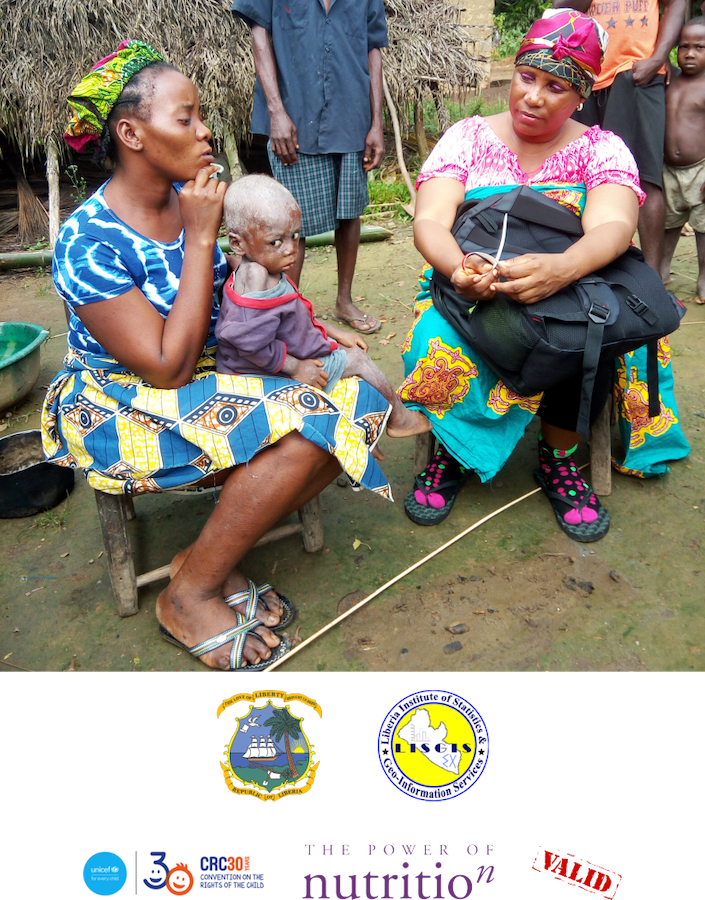
\includegraphics{figures/frontCoverLogos.png}\\[\bigskipamount]
}
\posttitle{\end{center}}
\usepackage{booktabs}
\usepackage{longtable}
\usepackage{array}
\usepackage{multirow}
\usepackage{wrapfig}
\usepackage{float}
\usepackage{colortbl}
\usepackage{pdflscape}
\usepackage{tabu}
\usepackage{threeparttable}
\usepackage{threeparttablex}
\usepackage[normalem]{ulem}
\usepackage{makecell}
\usepackage{xcolor}

\begin{document}
\maketitle

\newpage 

\pagenumbering{arabic}

{
\hypersetup{linkcolor=black}
\setcounter{tocdepth}{3}
\tableofcontents
}
\listoftables
\listoffigures
\newpage

\hypertarget{acknowledgements}{%
\section*{Acknowledgements}\label{acknowledgements}}
\addcontentsline{toc}{section}{Acknowledgements}

We are indebted to all the data collection teams who made this assessment possible, including data collectors, supervisors, and management teams from Ministry of Health, Liberia Institute of Statistics and Geo-Information Services and UNICEF Liberia. We are thankful for all the study participants - the mothers and children - who participated in the survey for their time and patience in providing information needed for this study. Without them, this study would not have been possible.

\newpage

\hypertarget{acronyms-and-abbreviations}{%
\section*{Acronyms and abbreviations}\label{acronyms-and-abbreviations}}
\addcontentsline{toc}{section}{Acronyms and abbreviations}

\begin{longtable}{ll}
\toprule
\textbf{Acronyms/Abbreviations} & \textbf{Definition}\\
\midrule
ANC & Antenatal care\\
CMAM & Community-based management of acute malnutrition\\
DHS & Demographic and health surveys\\
GAM & Global acute malnutrition\\
IDW & Inverse distance weighting\\
\addlinespace
IFA & Iron-folic acid\\
IU & International units\\
IYCF & Infant and young child feeding\\
MAM & Moderate acute malnutrition\\
MICS & Multiple indicator cluster survey\\
\addlinespace
MNP & Micronutrient powder\\
MUAC & Middle upper arm circumference\\
ODK & Open data kit\\
PoN & Power of Nutrition\\
PSU & Primary sampling unit\\
\addlinespace
SAM & Severe acute malnutrition\\
SMART & Standardized Monitoring and Assessment of Relief and Transitions\\
UNICEF & United Nations Children's Fund\\
\bottomrule
\end{longtable}

\newpage

\hypertarget{executive-summary}{%
\section*{Executive Summary}\label{executive-summary}}
\addcontentsline{toc}{section}{Executive Summary}

A three-year nutrition programme has been implemented in Liberia by UNICEF aimed at tackling child undernutrition in the country. Funded by \href{http://www.powerofnutrition.org}{Power of Nutrition} and \href{https://www.unicef.org.uk}{UNICEF UK}, the programme has been implemented across 15 counties in Liberia starting from January 2017 up to December 2019. The overall aim of the programme is to improve the coverage of direct nutrition interventions or what is commonly termed nutrition-specific interventions, i.e.~interventions or programmes that address the immediate determinants of foetal and child nutrition and development --- adequate food and nutrient intake, feeding, caregiving and parenting practices, and low burden of infectious diseases \citep{Bhutta:2013ks, Ruel:2013kr}. The current programme supports the following specific key interventions: 1) \emph{treatment of severe acute malnutrition (SAM) for children 6-59 months}; 2) \emph{vitamin A supplementation for children 6-59 months}; 3) \emph{promotion of appropriate infant and young child feeding (IYCF) practices among pregnant or lactating women}; 4) \emph{multiple micronutrient powder (MNP) supplementation for children 6-23 months}; and, 5) \emph{iron and folic acid (IFA) supplementation for pregnant women}.

The coverage assessment was implemented as a two-stage spatial sample survey with \(m = 30\) primary sampling units per programme area. A complete enumeration of children 6-59 months old from \(m = 30\) primary sampling units (PSUs) per programme area was performed in order to find all children who are severe acute malnourished (SAM) using standard case definitions for the community-based management of acute malnutrition (CMAM) programme coverage assessment. Within this cohort of children 6-59 months, a systematic sample of children and their mothers were selected for the coverage assessment of the other four nutrition-specific interventions. A total of at least \(n = 192\) children 6-23 months old for the micronutrient powder (MNP) supplementation coverage, children 6-59 months for vitamin A supplementation coverage and mothers of children 6-59 months for the infant and young child feeding (IYCF) counselling coverage and iron and folic acid (IFA) coverage were systematically selected. A set of hierarchical coverage indicators was used to assess coverage of each of the five nutrition-specific programmes. Data was collected using a specifically-designed Open Data Kit (ODK) data collection system. Data was analysed using R language for statistical computing. A blocked-weighted bootstrapping approach was used to estimate the various coverage indicators and to report the corresponding 95\% confidence interval. Indicators were also mapped using spatial interpolation using inverse distance weighting.

The results of the coverage assessment of direct nutrition interventions in Liberia specifically in Greater Monrovia and Grand Bassa indicate various levels of disparity in coverage both between the programme areas and within the programme areas assessed. Long-standing programmes such as IFA supplementation, IYCF counselling and vitamin A supplementation have performed fairly well in terms of coverage. The majority of women and children targeted by these programmes are knowledgeable of the programme and are beneficiaries of the programme. Years of implementation complemented by the level of support and investment by the government and its partners seem to have paid dividends in allowing for these programmes to reach almost all of their targeted beneficiaries. However, there is still much room for improvement and the current coverage levels can still be increased.

Programmes such as MNP and CMAM, on the other hand, show how new and recently scaled-up programmes are still in the process of achieving the highest levels of coverage possible. MNP supplementation which is the newest programme of those assessed is understandably still struggling with coverage even at endline. Knowledge of the programme and knowlege of how the programme works and its importance for children's health and nutrition is the key falter point which is typical of a programme at this stage of its evolution. The programme is mainly anchored to the health centre and therefore knowledge and access to it is primarily influenced by mothers' behaviours and attitudes towards seeking care and treatment at the health facility. Given that MNP is aimed at children who are otherwise healthy (not acute malnourished), the current MNP coverage estimates indicate that health-seeking behaviour leading to a visit to a health facility is mainly influenced by whether their children are sick rather than as a way to seek information or participate in promotive and preventive services such as MNP supplementation. Other factors include physical access to health centres. A more community-based approach to MNP supplementation that is integrated with other community-based programmes such as vaccinations and CMAM should be considered as a potential delivery mechanism. Screening of children using MUAC can be integrated into vaccination campaigns and children under 2 years old identified as not being acutely malnourished are informed about MNP supplementation programme and ideally provided with the MNP supplements at point of contact.

Finally, for CMAM which is not entirely new but still in its early stages of scale-up, the coverage estimates at baseline and endline indicate 1) disparity between Greater Monrovia and Grand Bassa in terms of the level and intensity of the community aspects of the programme; 2) signficant drop in coverage of CMAM in Greater Monrovia given that at baseline its coverage was exemplary for an urban CMAM programme; and, 3) no significant change in coverage of CMAM in Grand Bassa with coverage still remaining unacceptably low. At baseline, screening and case-finding in Greater Monrovia is better than in Grand Bassa and this can partly explain the difference in treatment coverage between the two areas at baseline. At endline, no improvement in screening has happened and the levels of coverage for CMAM in Greater Monrovia has signficantly plummetted. Based on feedback by stakeholders, this has been attributed to government being the main service provider for CMAM in the past year as usual stakeholders that supported government were not engaged due to several programmatic issues. This points to the need for ensuring increased and continued capacity building of government in CMAM and other related interventions so that they can be truly in a position that they can implement and maintain these programmes with or without external support.

Lessons learned from the years of implementation of the IFA and vitamin A programmes can be useful in improving coverage of MNP and CMAM particularly with potential integration of these services into a unified and coherent child health and nutrition programme in Liberia.

\newpage

\hypertarget{intro}{%
\section{Introduction}\label{intro}}

A three-year nutrition programme has been implemented in Liberia by UNICEF aimed at tackling child undernutrition in the country. Funded by \href{http://www.powerofnutrition.org}{Power of Nutrition} and \href{https://www.unicef.org.uk}{UNICEF UK}, the programme has been implemented across 15 counties in Liberia starting from January 2017 up to December 2019. The overall aim of the programme is to improve the coverage of direct nutrition interventions or what is commonly termed nutrition-specific interventions, i.e.~interventions or programmes that address the immediate determinants of foetal and child nutrition and development --- adequate food and nutrient intake, feeding, caregiving and parenting practices, and low burden of infectious diseases \citep{Bhutta:2013ks, Ruel:2013kr}. The current programme supports the following specific key interventions: 1) \emph{treatment of severe acute malnutrition (SAM) within the community-based management of acute malnutrition (CMAM) programme for children 6-59 months}; 2) \emph{vitamin A supplementation for children 6-59 months}; 3) \emph{promotion of appropriate infant and young child feeding (IYCF) practices among pregnant or lactating women}; 4) \emph{multiple micronutrient powder (MNP) supplementation for children 6-23 months}; and, 5) \emph{iron and folic acid (IFA) supplementation for pregnant women}.

To assess the programme's progress towards its overall aim, two coverage assessments have been implemented - the first at the halfway point of the programme and the second at the end. Only two programme areas were selected for the assessments: \emph{Urban Montserrado (Greater Monrovia)} district and \emph{Grand Bassa} county. This report presents the results of these assessments.

\hypertarget{methods}{%
\section{Methods}\label{methods}}

\hypertarget{sample-design}{%
\subsection{Survey and sampling design}\label{sample-design}}

The coverage assessment was designed to be spatially representative of each of the two programme areas using a two-stage spatial sampling survey approach. An even spatial distribution of primary sampling units (PSUs) (i.e., villages/enumeration areas/city blocks) was selected from across each enumeration area. This approach was used in order to assess coverage and its spatial distribution in order to detect and map heterogeneity of coverage \citep{Elliott:2004cg, Diggle:2014tk}. PSUs were selected based on their proximity to centroids of a hexagonal grid laid over the two selected programme areas resulting in a triangular irregular network \citep{Isaaks:1989uk, Elliot:2000vs}. A complete enumeration of children 6-59 months old from \(m = 30\) PSUs per programme area was performed in order to find all children who are SAM based on specified case definitions\footnote{Initial design used both weight-for-height z-score (WHZ) and MUAC and oedema criteria for SAM. However, for the first round of coverage assessments in 2018, the survey technical team decided to use MUAC and oedema only for SAM case-finding during the survey given the length of time it took to perform complete enumeration using WHZ. For the second round of coverage assessments in 2019, WHZ, MUAC and oedema case definitions for SAM were used.} for the CMAM programme coverage assessment. Within this cohort of children 6-59 months, a systematic sample of children and their mothers were selected for the coverage assessment of the other four nutrition-specific interventions. A total of at least \(n = 192\) children 6-23 months old for the MNP supplementation coverage, children 6-59 months for vitamin A supplementation coverage and mothers of children 6-59 months for the IYCF counselling coverage and IFA coverage were systematically selected. A detailed description of the sampling design can be found \href{https://validmeasures.org/liberiaS3M/}{here}.

\hypertarget{indicators}{%
\subsection{Indicators}\label{indicators}}

The coverage assessment evaluated the following indicators.

\hypertarget{cmam-coverage}{%
\subsubsection{CMAM coverage}\label{cmam-coverage}}

CMAM coverage usually pertains to coverage of SAM treatment. Historically, there have been two coverage estimators in common use: \textbf{point} and \textbf{period} coverage.

Point coverage is the number of current SAM cases in a treatment programme divided by the total number of current SAM cases.

\textbf{Point coverage} uses data for current cases only. It is calculated using the following formula:

\$nbsp;

\[\begin{aligned} 
\text{Point coverage} & ~ = ~ \frac{C_{in}}{C_{in} ~ + ~ C_{out}} \\
\\
where: & \\
\\
C_{in} & ~ = ~ \text{current SAM cases in the programme} \\
C_{out} & ~ = ~ \text{current SAM cases out of the programme}
\end{aligned}\]

~

\textbf{Point coverage} provides a snapshot of programme performance, putting a strong emphasis on the effectiveness and timeliness of case-finding and recruitment \citep{Myatt:2012tt}.

\textbf{Period coverage}, on the other hand, uses data for both current and recovering cases. It is calculated using the following formula:

~

\[\begin{aligned}
\text{Period coverage} & ~ = ~ \frac{C_{in} ~ + ~ R_{in}}{C_{in} ~ + ~ C_{out} ~ + ~ R_{in}} \\
\\
where: & \\
\\
R_{in} & ~ = ~ \text{recovering SAM cases in the programme}
\end{aligned}\]

~

\textbf{Period coverage} is the number of current and recovering cases in a treatment programme divided by all current SAM cases and recovering cases. It approximates treatment coverage much better (albeit with limitations) as it accounts for children who are no longer cases but are in the programme.

However, given the known limitations of point and period coverage \citep{Myatt:2012tt}, the single coverage estimator proposed and recommended by \citet{Balegamire:2015ud} was used as the CMAM programme coverage estimators. Also, given the single coverage estimator, we adopted a shift in terminology that is more descriptive and specific with regard to what the estimator is actually measuring, allowing both measures to be reported together without confusion. \textbf{Point coverage} was termed \emph{case-finding effectiveness} to more precisely reflect it as a measure of the programme's ability to find and recruit current cases. This indicator assesses how good the treatment programme is in finding cases of SAM and then getting them to treatment. \textbf{Period coverage} that has been improved into the single coverage metric was named \emph{treatment coverage} as this is the estimator that approximates this coverage indicator the closest.

\hypertarget{vitamin-a-supplementation}{%
\subsubsection{Vitamin A supplementation}\label{vitamin-a-supplementation}}

The standard estimator for vitamin A supplementation is the proportion of children aged 6-59 months who received two age-appropriate doses of vitamin A in the past 12 months.

In standard surveys such as the Demographic and Health Surveys (DHS) and the Multiple Indicator Cluster Surveys (MICS), this indicator is adjusted to a recall of 6 months for a single age-appropriate dose of vitamin A. This was the indicator used for this assessment.

Age appropriate vitamin A supplementation was assessed mainly through mother's recall of which gel capsule the child received recently. The blue vitamin A gel capsule containing 100,000 IU of vitamin A is given to children 6-11 months. The red vitamin A gel capsule containing 200,000 IU of vitamin A is given to children 12 - 59 months. A photo of the blue and the red gel capsule was used to aid the mother/caregiver in answering this question.

\hypertarget{iron-folic-acid-ifa-supplementation-for-pregnant-women}{%
\subsubsection{Iron-folic acid (IFA) supplementation for pregnant women}\label{iron-folic-acid-ifa-supplementation-for-pregnant-women}}

Population-based surveys typically report the percentage of women with a live birth in the two to five years before the survey who received and took IFA supplementation during their most recent pregnancy. Because antenatal care (ANC) is the main platform for IFA supplement distribution for pregnant women, survey questions on antenatal care attendance was used to provide information on the use of this platform to deliver IFA supplementation. \citet{Sununtnasuk:2015kb} proposed a falter point framework\footnote{Similar to a bottleneck framework and consistent with \citet{Tanahashi:1978we} hierarchical model of coverage.} that utilises four indicators that proxy the five critical points at which the ANC approach to IFA distribution might falter in IFA supplementation coverage to pregnant women. These indicators are:

\begin{enumerate}
\def\labelenumi{\arabic{enumi}.}
\item
  At least one ANC visit during most recent pregnancy
\item
  Knowledge of IFA tablet/s
\item
  Receipt or purchase of IFA tablet/s
\item
  IFA consumption
\item
  Adherence to at least 90 days of supplementation
\end{enumerate}

\hypertarget{micronutrient-powder-supplementation}{%
\subsubsection{Micronutrient powder supplementation}\label{micronutrient-powder-supplementation}}

The indicator for coverage of micronutrient powder supplementation is the proportion of children aged 6-23 months who consume micronutrient powder supplements. An indicator set on MNP supplementation was devised similar to the IFA supplementation falter point or bottleneck framework that first assessed knowledge and awareness of MNP supplementation, then the receipt/purchase of MNP and finally consumption of MNP.

\hypertarget{iycf-counselling}{%
\subsubsection{IYCF counselling}\label{iycf-counselling}}

There are no standard indicators for IYCF counselling hence indicators were devised based on how this intervention was being delivered to pregnant or lactating women. In terms of mechanism, these sessions are delivered via the health clinic/health post and that the target beneficiaries are pregnant or lactating women. Given this, similar approach to the IFA supplementation coverage of falter points/bottle necks was used with the following indicators:

\begin{enumerate}
\def\labelenumi{\arabic{enumi}.}
\item
  At least one ANC visit during most recent pregnancy
\item
  Awareness of IYCF counselling
\item
  Attendance at IYCF counselling
\end{enumerate}

\hypertarget{survey-instrument}{%
\subsection{Survey instrument}\label{survey-instrument}}

Two sets of survey instruments were produced for the survey. The first is for the CMAM coverage component and the second one is for the survey for children 6-59 months and their mothers. The sample/template questionnaires used can be found in Annex A.

\hypertarget{using-open-data-kit}{%
\subsubsection{Using Open Data Kit}\label{using-open-data-kit}}

Based on the template forms described above, a digital data collection system using Open Data Kit (ODK) was developed. These forms are available as a \href{https://github.com/validmeasures/liberiaS3Mforms}{Github repository}. The system is composed of two forms.

\hypertarget{village-form}{%
\paragraph{Village form}\label{village-form}}

This form (\texttt{liberiaCoverageVillageForm.xlsx} and \texttt{liberiaCoverageVillageForm.xml}) collected information on the villages or primary sampling units (PSU) selected for the Liberia Coverage Survey. This information includes:

\begin{enumerate}
\def\labelenumi{\arabic{enumi}.}
\item
  County name (and identifier)
\item
  Village name (and identifier)
\item
  Village population size
\item
  Village geocoordinates
\end{enumerate}

\hypertarget{coverage-form}{%
\paragraph{Coverage form}\label{coverage-form}}

This form (\texttt{liberiaCoverage.xlsx} and \texttt{liberiaCoverage.xml}) collected information on the various coverage indicators assessed in the Liberia Coverage Survey:

\begin{enumerate}
\def\labelenumi{\arabic{enumi}.}
\item
  CMAM coverage
\item
  Iron-folic acid supplementation coverage
\item
  IYCF counselling coverage
\item
  Micronutrient powder supplementation coverage
\item
  Vitamin A supplementation coverage
\end{enumerate}

The coverage form was developed in such a way that it implements the survey as per survey design such that the modules for IFA coverage, IYCF counselling coverage, MNP supplementation coverage and vitamin A supplementation coverage are only shown based on the sampling interval for a particular primary sampling unit (PSU) and based on the different eligibility requirements for each coverage survey module.

\hypertarget{data-analyses}{%
\subsection{Data analyses}\label{data-analyses}}

Data analysis was performed using R language for statistical computing \citep{R:2019rr}. An R package called \texttt{liberiaData} containing specific functions for data processing and analysis of the Liberia coverage survey was produced to ensure open availability of data and reproducibility of analysis\footnote{See package site at \url{https://validmeasures.org/liberiaData/} for more information and for instructions on installation and usage}. An auxiliary R package called \texttt{liberia} containing additional secondary data including maps used for the sampling and survey process was also produced\footnote{See package site at \url{https://validmeasures.org/liberia/} for more information and for instructions on installation and usage}.

\hypertarget{analytical-approach-for-estimating-coverage-indicators}{%
\subsubsection{Analytical approach for estimating coverage indicators}\label{analytical-approach-for-estimating-coverage-indicators}}

Data analysis procedures accounted for the sample design.

\begin{itemize}
\item
  This survey is a two-stage sample. Subjects are sampled from a small number of PSUs.
\item
  This survey is \textbf{not} prior weighted. This means that per-PSU sampling weights will be needed. These are usually the populations of the PSU.
\end{itemize}

For this survey, the \emph{blocked weighted bootstrap} estimation approach was used:

\begin{itemize}
\item
  \textbf{Blocked} : The block corresponds to the PSU or cluster.
\item
  \textbf{Weighted} : The sampling procedure for this survey does not use population proportional sampling (PPS) to weight the sample prior to data collection as is done with SMART type surveys. This means that a posterior weighting procedure is required. The ``roulette wheel'' algorithm to weight (i.e.~by population) the selection probability of PSUs in bootstrap replicates will be utilised.
\end{itemize}

A total of \texttt{m} PSUs are sampled \emph{with-replacement} from the survey dataset where \texttt{m} is the number of PSUs in the survey sample. Individual records within each PSU are then sampled \emph{with-replacement}. A total of n' records are sampled \emph{with-replacement} from each of the selected PSUs where \texttt{n} is the number of individual records in a selected PSU. The resulting collection of records replicates the original survey in terms of both sample design and sample size. A large number of replicate surveys are taken (minimum of \(r = 399\) replicate surveys but this can be changed). The required statistic (e.g.~the mean of an indicator value) is applied to each replicate survey. The reported estimate consists of the 50th (point estimate), 2.5th (lower 95\% confidence limit), and the 97.5th (upper 95\% confidence limit) percentiles of the distribution of the statistic observed across all replicate surveys. The blocked weighted bootstrap procedure is outlined in Figure \ref{fig:indicators31}.

The principal advantages of using a bootstrap estimator are:

\begin{itemize}
\item
  Bootstrap estimators work well with small sample sizes.
\item
  The method is \emph{non-parametric} and uses empirical rather than theoretical distributions. There are no assumptions of things like normality to worry about.
\item
  The method allows estimation of the sampling distribution of almost any statistic using only simple computational methods.
\end{itemize}

\newpage

\begin{figure}[H]

{\centering 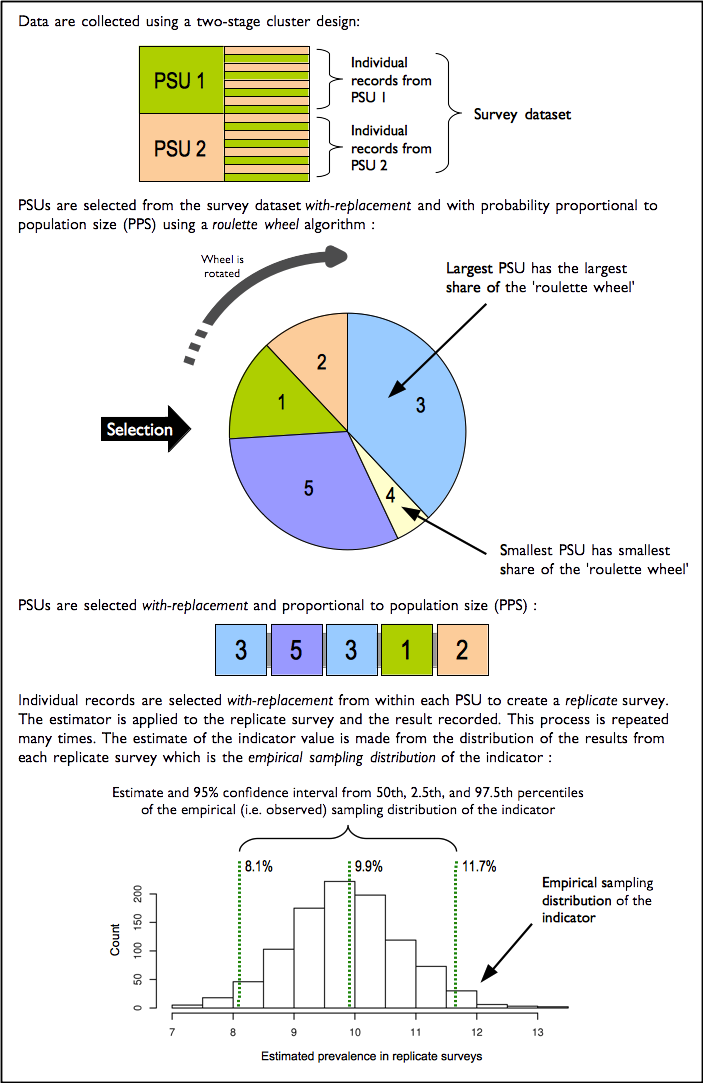
\includegraphics[width=9.76in]{figures/bbw} 

}

\caption{The blocked weighted bootstrap}\label{fig:indicators31}
\end{figure}

\hypertarget{analytical-approach-for-mapping-coverage-indicators}{%
\subsubsection{Analytical approach for mapping coverage indicators}\label{analytical-approach-for-mapping-coverage-indicators}}

The indicator mapping approach for this survey created a surface map of indicator values using spatial interpolation. There are various approaches and methods of spatial interpolation, the main differences are determined by the weights applied to the point dataset to estimate values at each of the unknown points of the surface map. For the Liberia coverage survey, spatial interpolation was performed using the inverse distance weighting (IDW) method. As the name implies, the IDW method uses weights that are inversely proportional to the distance of a point being estimated from the sampling point locations \citep{Isaaks:1989uk, diggle2007mbg, diggle2013statistical}. This can be mathematically demonstrated as follows:

\[\begin{aligned}
\hat{v} & ~ = ~ \frac{\displaystyle \sum\limits_{i ~ = ~ 1} ^ {n} \frac{1}{d_{i}^{p}}v_{i}}{\displaystyle \sum\limits_{i ~ = ~ 1}^{n}\frac{1}{d_{i}^{p}}} \\
\\
where: & \\
\\
d_1 \ldots d_n & ~ = ~ \text{distances from each } n \text{ sampling points to estimation point} \\
p & ~ = ~ \text{power of the distance} \\
v_1 \ldots v_n & ~ = ~ \text{sample values}
\end{aligned}\]

The power of the distance \texttt{p} is an important aspect of the IDW method for point estimation. The influence of \texttt{p} to the weights applied to the point estimation is such that as \texttt{p} approaches 0, the weights become more similar, thereby giving more weight to the nearest sample values. As \texttt{p} approaches \(\infty\), the weights become more different from each other, thereby giving more weight to the closest sample. The power of the distance \texttt{p} has been traditionally set at 2 for convenience and ease of calculations. For the Liberia Coverage Survey, \texttt{p} was initially set at 2 and then cross-validation (see below) was applied to optimise \texttt{p} to a value that minimises the estimation errors at each of the sampling point locations.

Cross-validation is a technique applied to validate predictive models. It assesses how accurately the predictive model performs in practice. IDW is one of the simplest model-based interpolation methods available, but ideally would still require a form of cross-validation to determine the optimal value of the distance power \texttt{p} (described above).

A two-fold cross validation \citep{bivand2008applied} was applied to the Liberia coverage data wherein data points were randomly split into two sets of equal size, with one set assigned as the validation data for testing the model, and the other set as the training data. The validation data was then interpolated using the IDW method with an initial \texttt{p} of 2 and the resulting predictions were compared with the training data. Comparison was made using the sum of the squared residuals between the predicted values and the observed values to report errors. Optimisation was then performed by replicating the two-fold cross validation process 100 times using randomly generated values for \texttt{p}. Out of these replicates, the value of \texttt{p} that provided prediction results with the minimum errors was selected as the distance power for the eventual interpolation performed.

\hypertarget{results-and-discussion}{%
\section{Results and Discussion}\label{results-and-discussion}}

\hypertarget{iron-folic-acid-supplementation-coverage}{%
\subsection{Iron-Folic Acid Supplementation Coverage}\label{iron-folic-acid-supplementation-coverage}}

Figure \ref{fig:ifa1plot} and Table \ref{tab:ifa1table} presents a summary of the IFA supplementation coverage indicators for Greater Monrovia and Grand Bassa at baseline and endline. The majority of mothers surveyed at baseline and endline from Greater Monrovia and Grand Bassa have attended ANC during their last pregnancy, are aware of IFA tablets, have received IFA tablets and have consumed IFA tablets. Knowledge, receipt and consumption of IFA have all increased at endline compared to baseline with the increase being statistically significant in Greater Monrovia.

\begin{figure}[H]

{\centering 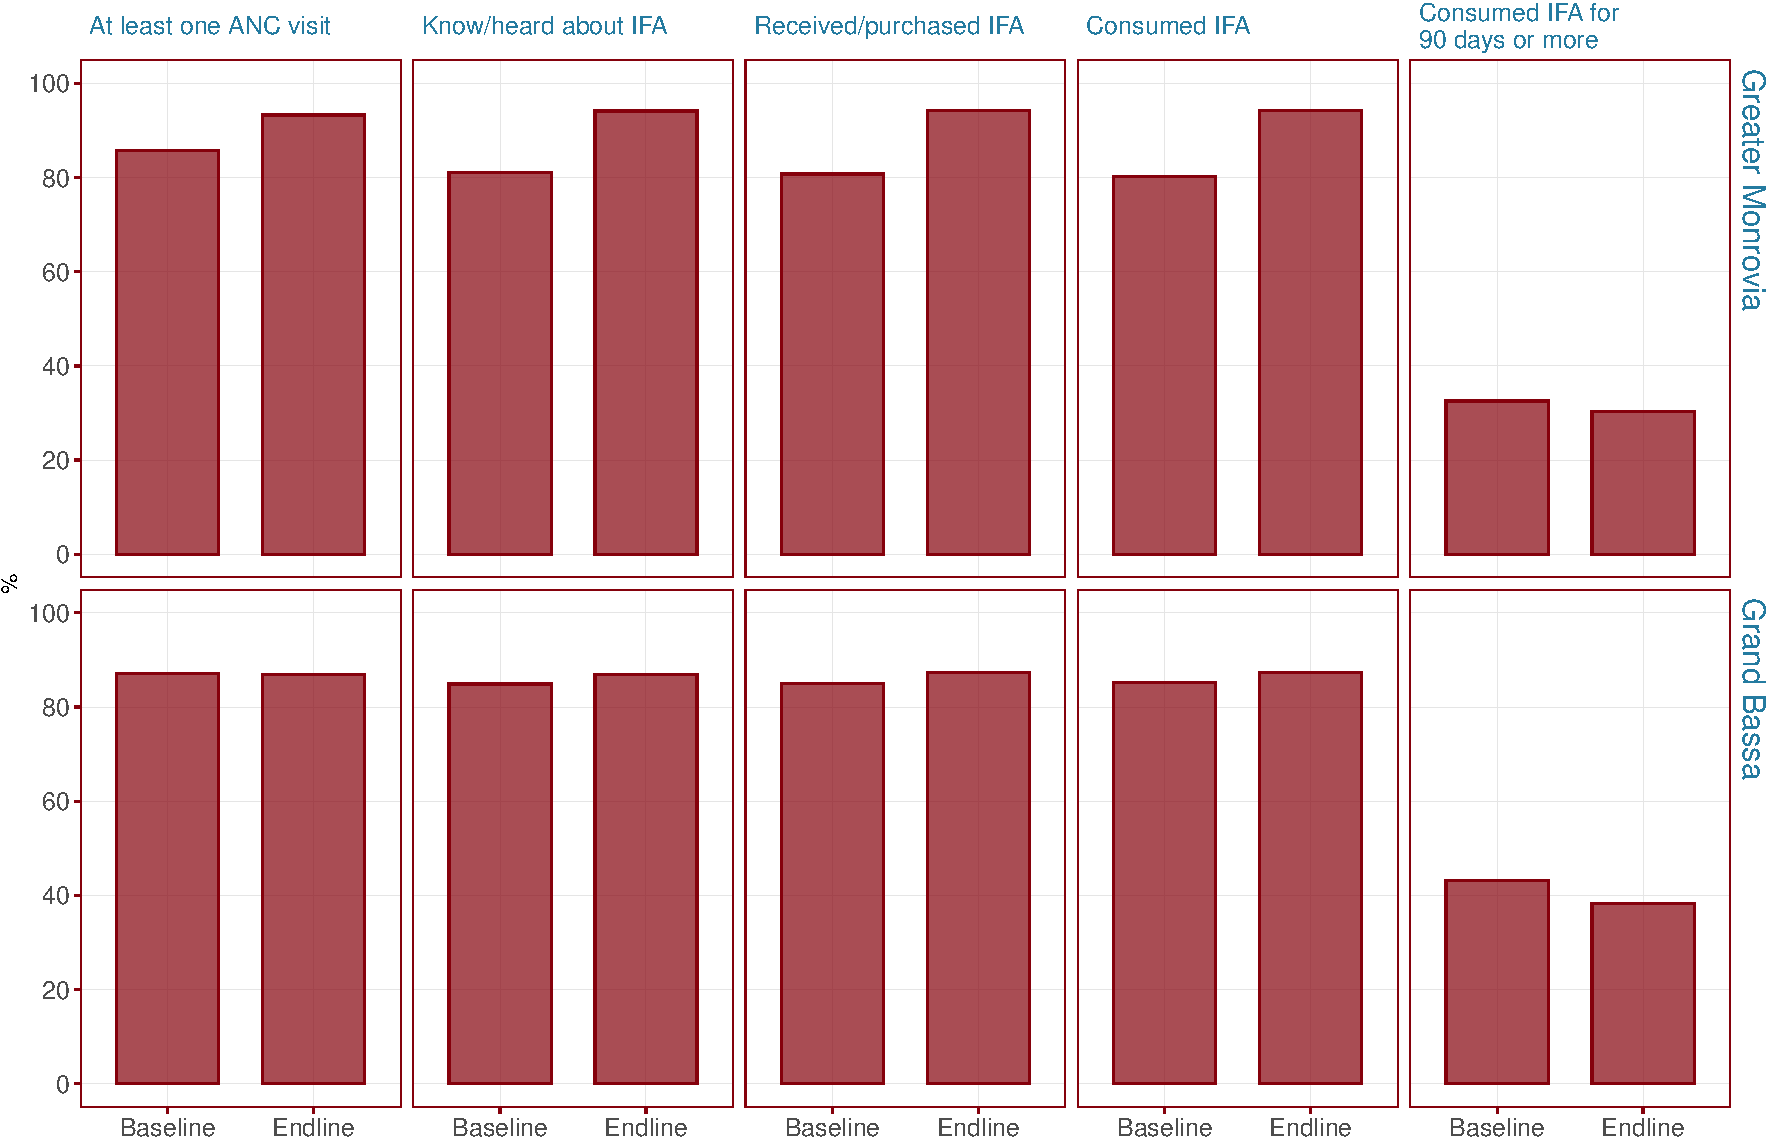
\includegraphics{liberiaCoverageFinalReport_files/figure-latex/ifa1plot-1} 

}

\caption{IFA supplementation coverage}\label{fig:ifa1plot}
\end{figure}

\begin{table}[H]

\caption{\label{tab:ifa1table}Iron-folic acid supplementation coverage}
\centering
\fontsize{9}{11}\selectfont
\begin{tabular}[t]{l>{\ttfamily}r>{\ttfamily}r>{\ttfamily}r>{\ttfamily}r>{\ttfamily}r>{\ttfamily}r>{\ttfamily}r>{\ttfamily}r>{\ttfamily}r>{\ttfamily}r>{\ttfamily}r>{\ttfamily}r}
\toprule
\multicolumn{1}{c}{\textbf{ }} & \multicolumn{6}{c}{\textbf{Greater Monrovia}} & \multicolumn{6}{c}{\textbf{Grand Bassa}} \\
\cmidrule(l{3pt}r{3pt}){2-7} \cmidrule(l{3pt}r{3pt}){8-13}
\multicolumn{1}{c}{\textbf{ }} & \multicolumn{3}{c}{\textbf{Baseline}} & \multicolumn{3}{c}{\textbf{Endline}} & \multicolumn{3}{c}{\textbf{Baseline}} & \multicolumn{3}{c}{\textbf{Endline}} \\
\cmidrule(l{3pt}r{3pt}){2-4} \cmidrule(l{3pt}r{3pt}){5-7} \cmidrule(l{3pt}r{3pt}){8-10} \cmidrule(l{3pt}r{3pt}){11-13}
\multicolumn{1}{c}{\textbf{Indicator}} & \multicolumn{1}{c}{\textbf{\makecell[c]{Est\\(\%)}}} & \multicolumn{1}{c}{\textbf{\makecell[c]{95\%\\LCL}}} & \multicolumn{1}{c}{\textbf{\makecell[c]{95\%\\UCL}}} & \multicolumn{1}{c}{\textbf{\makecell[c]{Est\\(\%)}}} & \multicolumn{1}{c}{\textbf{\makecell[c]{95\%\\LCL}}} & \multicolumn{1}{c}{\textbf{\makecell[c]{95\%\\UCL}}} & \multicolumn{1}{c}{\textbf{\makecell[c]{Est\\(\%)}}} & \multicolumn{1}{c}{\textbf{\makecell[c]{95\%\\LCL}}} & \multicolumn{1}{c}{\textbf{\makecell[c]{95\%\\UCL}}} & \multicolumn{1}{c}{\textbf{\makecell[c]{Est\\(\%)}}} & \multicolumn{1}{c}{\textbf{\makecell[c]{95\%\\LCL}}} & \multicolumn{1}{c}{\textbf{\makecell[c]{95\%\\UCL}}}\\
\midrule
\rowcolor{gray!6}  At least one ANC visit & 85.8 & 79.7 & 91.4 & 93.3 & 90.3 & 96.5 & 87.1 & 82.7 & 91.2 & 86.9 & 80.6 & 92.3\\
Know/heard about IFA & 81.1 & 73.2 & 87.0 & 94.1 & 91.0 & 97.1 & 84.9 & 80.0 & 89.0 & 86.9 & 81.3 & 91.8\\
\rowcolor{gray!6}  Received/purchased IFA & 80.7 & 73.7 & 86.8 & 94.2 & 91.1 & 97.1 & 85.0 & 79.4 & 89.4 & 87.3 & 81.4 & 92.6\\
Consumed IFA & 80.3 & 73.1 & 87.1 & 94.2 & 91.1 & 97.1 & 85.2 & 79.1 & 89.5 & 87.3 & 81.4 & 92.6\\
\rowcolor{gray!6}  Consumed IFA for 90 days or more & 32.6 & 20.8 & 43.0 & 30.3 & 24.1 & 36.8 & 43.2 & 33.6 & 52.0 & 38.2 & 27.5 & 50.0\\
\bottomrule
\end{tabular}
\end{table}

However, coverage of IFA faltered significantly in both areas when length (in days) of IFA tablet consumption was assessed with no improvement at endline compared to baseline (see Figure \ref{fig:ifaTanahashiPlot}).

\begin{figure}[H]

{\centering 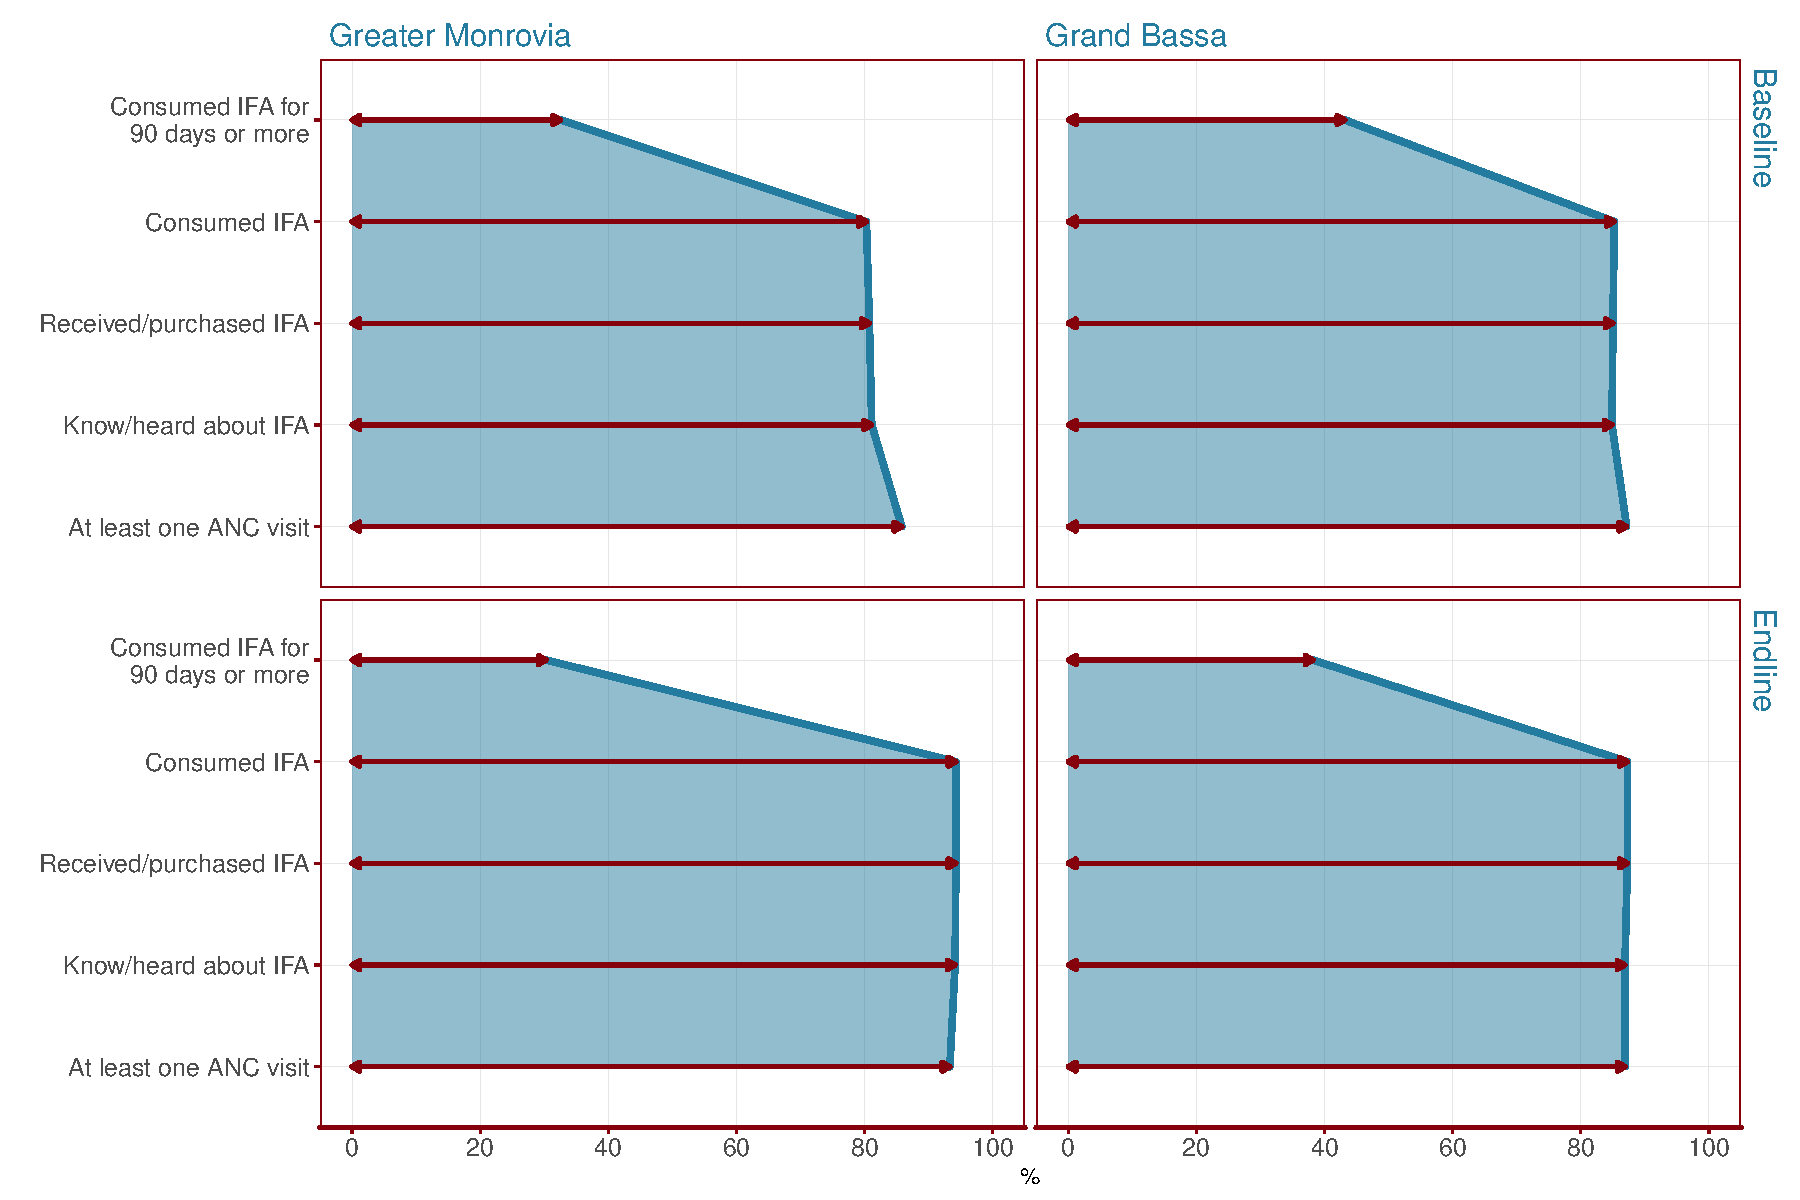
\includegraphics{liberiaCoverageFinalReport_files/figure-latex/ifaTanahashiPlot-1} 

}

\caption{Tanahashi plot for IFA supplementation coverage}\label{fig:ifaTanahashiPlot}
\end{figure}

Of the few who have not received IFA tablets in Greater Monrovia and Grand Bassa despite attending ANC during their last pregnancy, the main reasons for not getting IFA tablets are shown in Figure \ref{fig:ifa2plot}. At baseline, information regarding the IFA tablets was the main reason for non-coverage in both areas. At endline, difficulty in access and availability of IFA tablets at the clinics or hospital were the main reasons for non-coverage. This may mean that previous issue of lack of information was addressed over the past year but those who have learned about IFA tablets have struggled to gain access to the supplements.

\begin{figure}[H]

{\centering 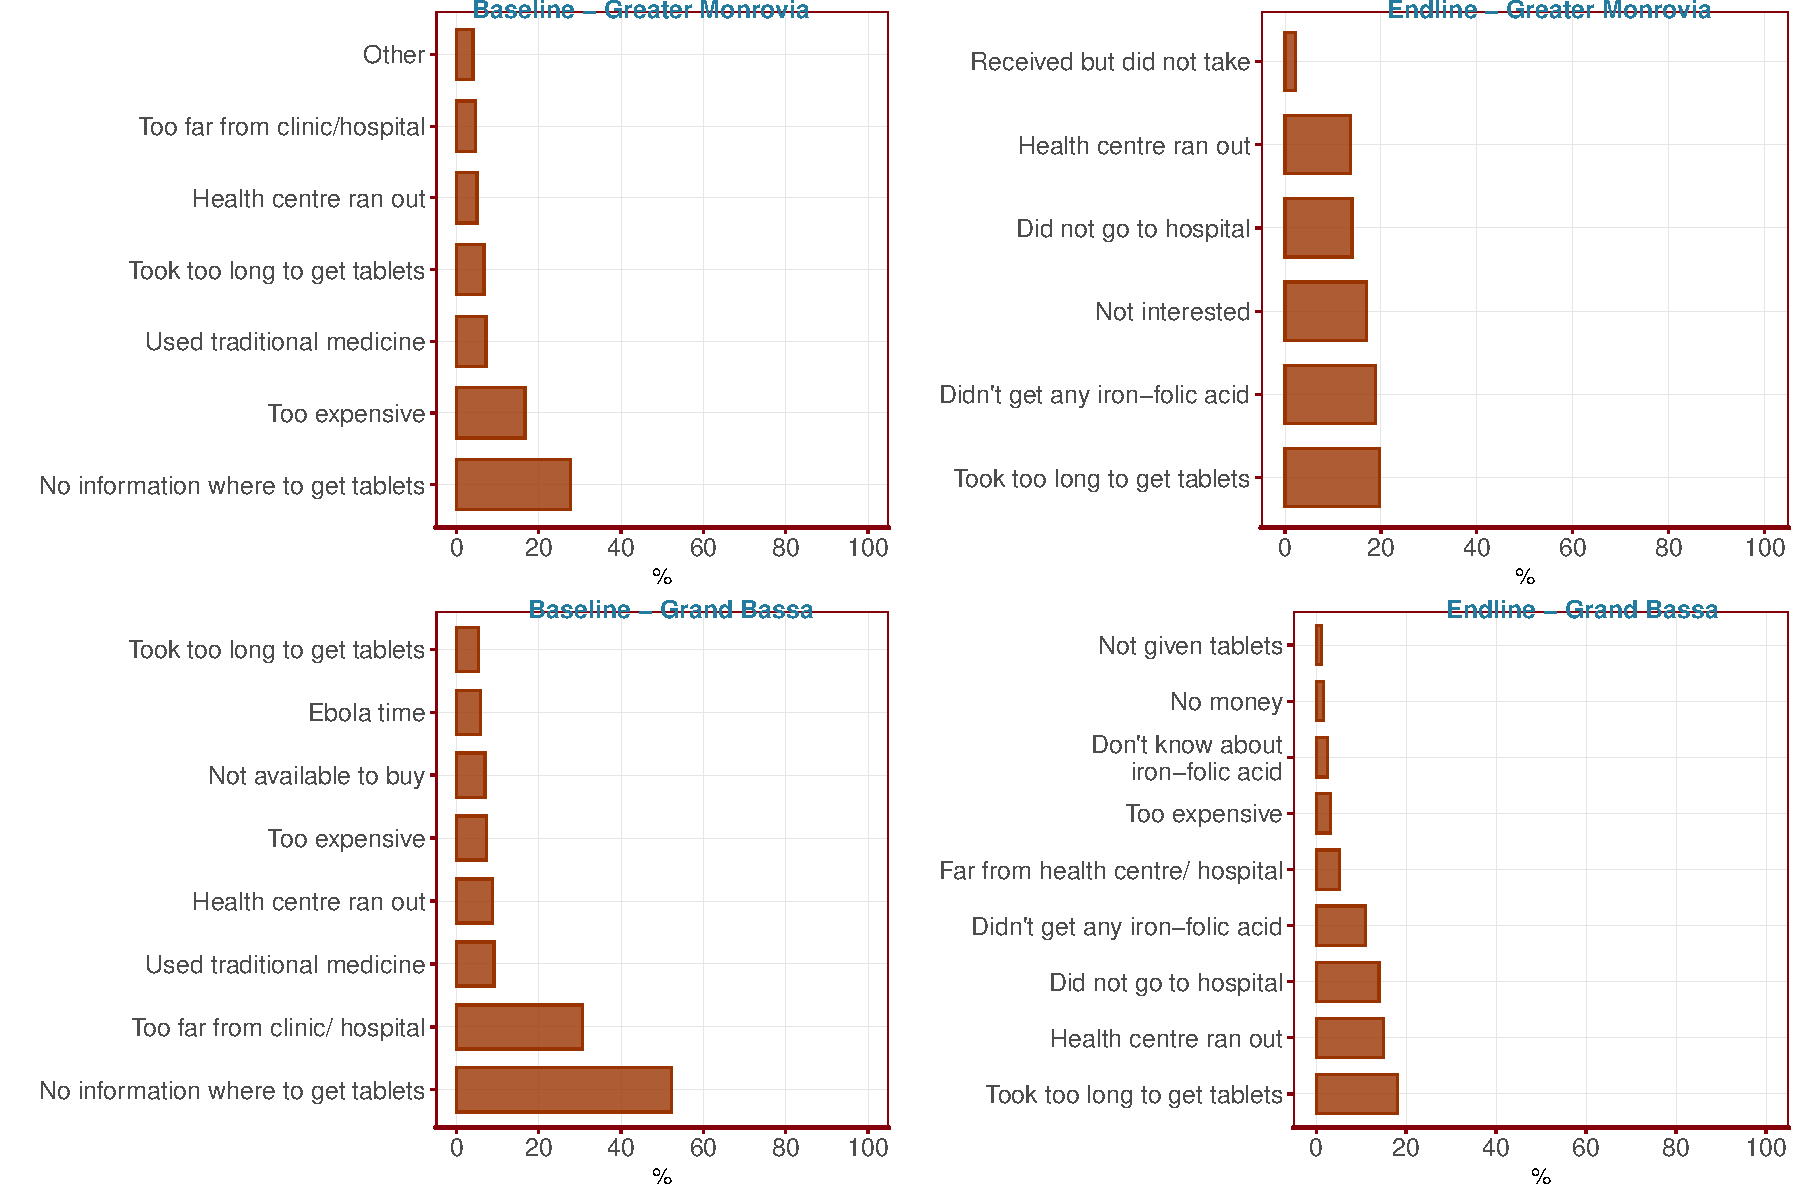
\includegraphics{liberiaCoverageFinalReport_files/figure-latex/ifa2plot-1} 

}

\caption{Reasons for not receiving/purchasing IFA supplementation}\label{fig:ifa2plot}
\end{figure}

The spatial distribution of IFA supplementation coverage in Greater Monrovia and Grand Bassa is shown in Figure \ref{fig:ifa1map} and \ref{fig:ifa2map}. At baseline, IFA supplementation coverage was lowest in the eastern section of Monrovia. At endline, these areas have increased coverage. For Grand Bassa, IFA supplementation coverage was lowest in the southern and eastern parts of the county. At endline, these areas have increased coverage but with new but much smaller hot spots of low coverage in different parts of the county. The maps for both Greater Monrovia and Grand Bassa show the significant faltering in IFA coverage once adequate consumption of IFA is considered consistent with the aggregated point estimates presented above.

\begin{figure}[H]

{\centering 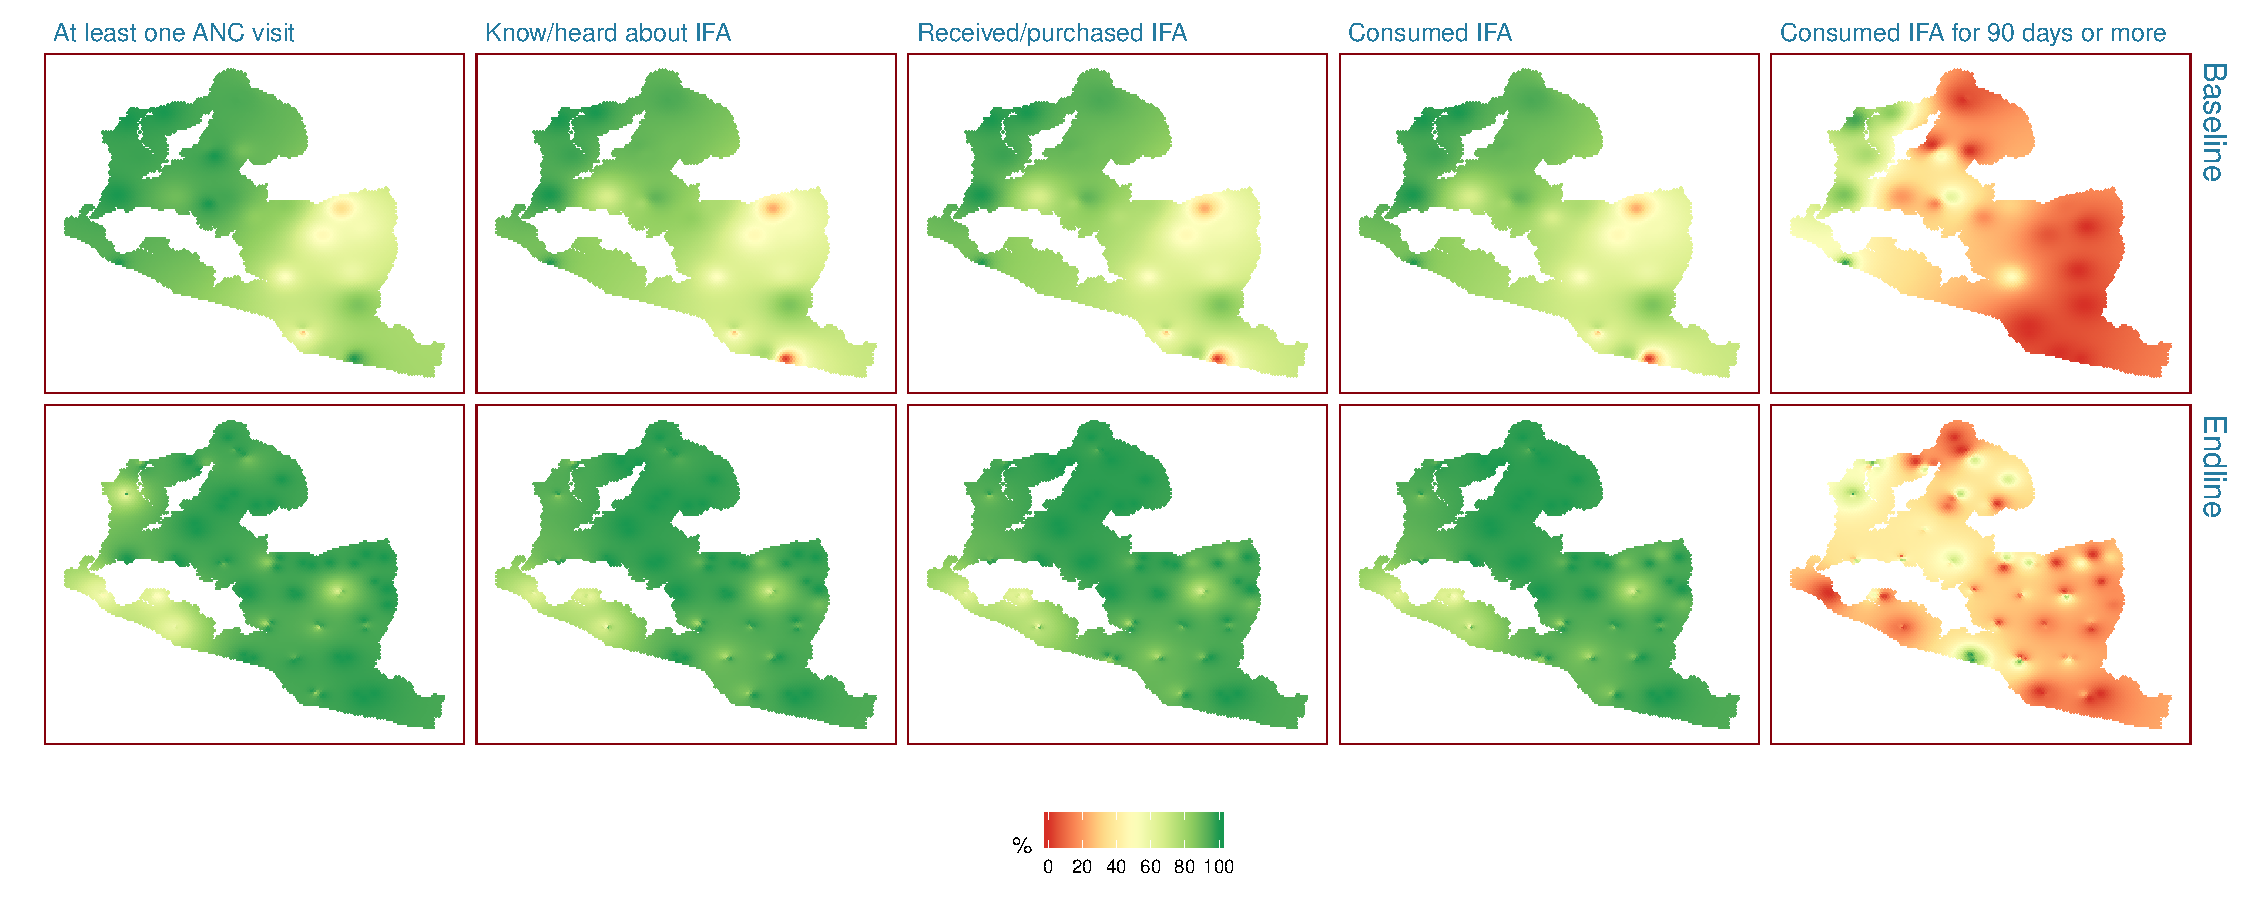
\includegraphics{liberiaCoverageFinalReport_files/figure-latex/ifa1map-1} 

}

\caption{Spatial distribution of IFA supplementation coverage in Greater Monrovia}\label{fig:ifa1map}
\end{figure}

\begin{figure}[H]

{\centering 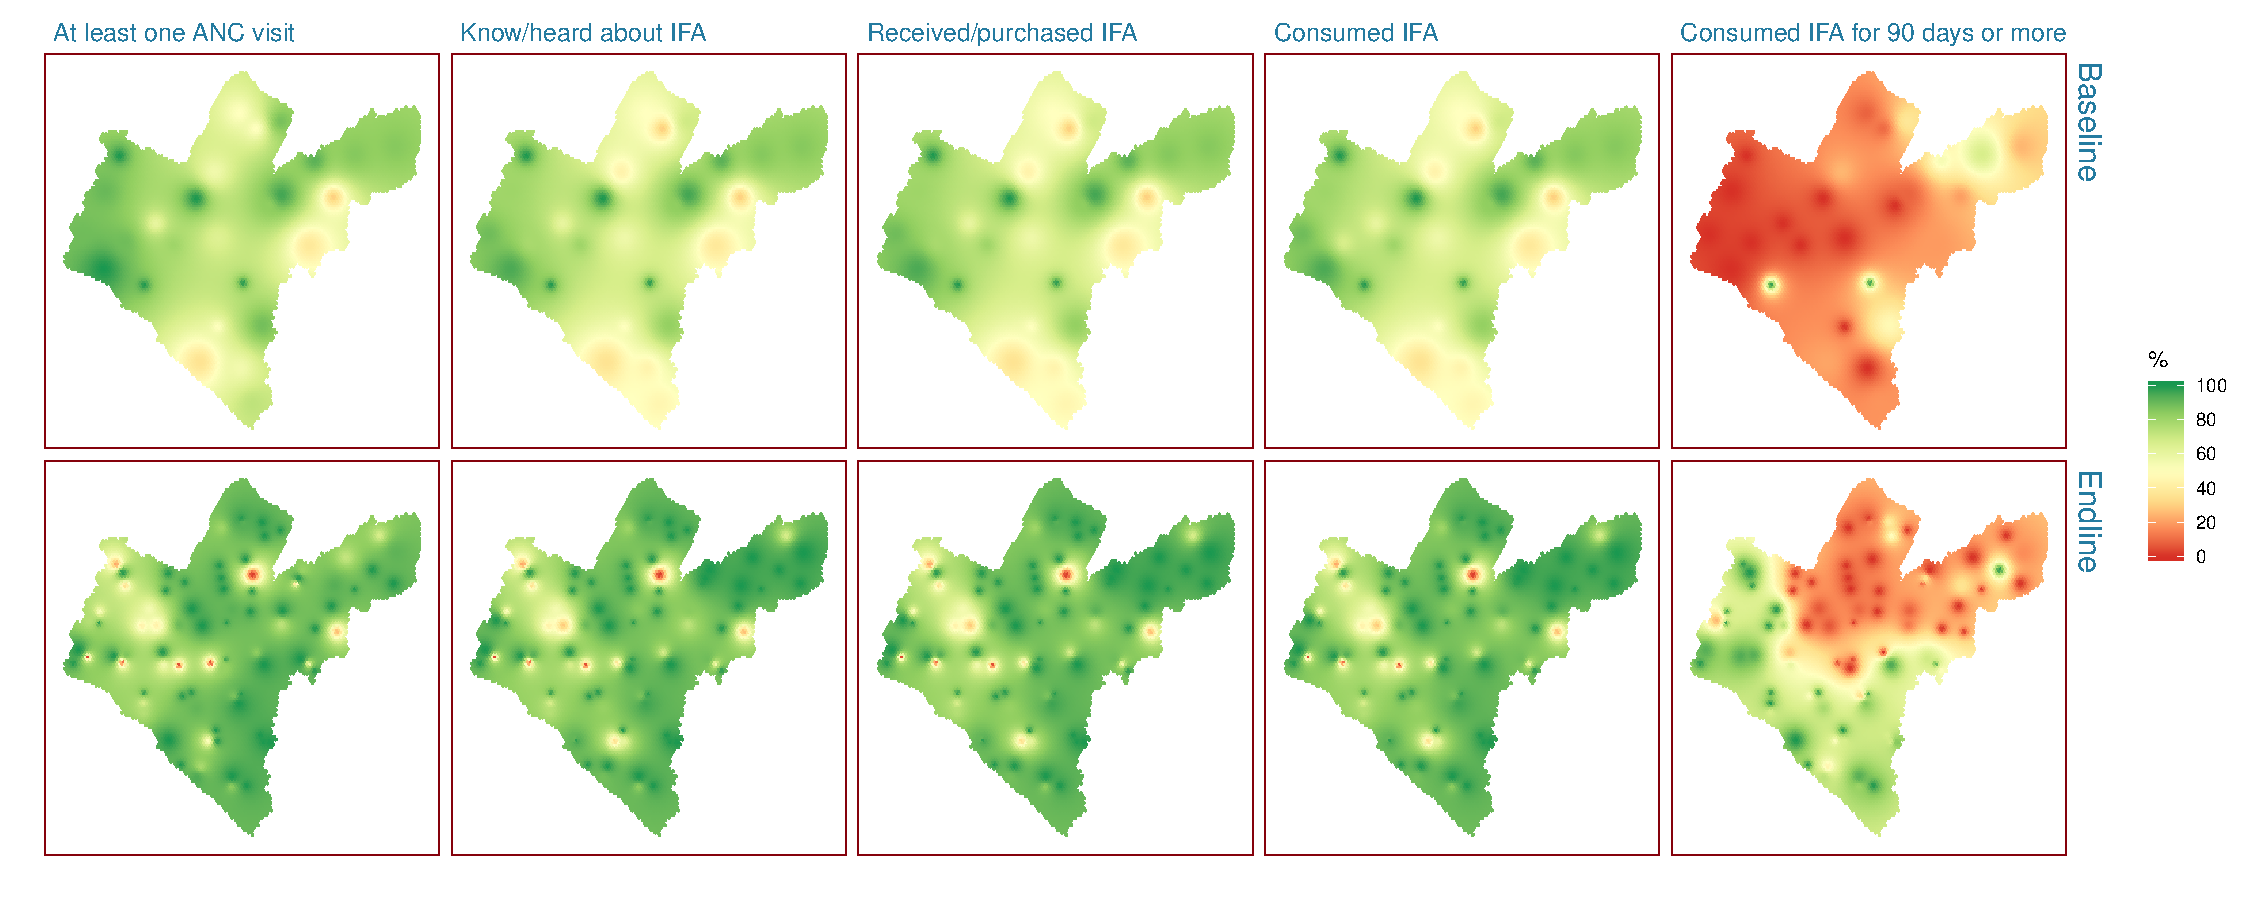
\includegraphics{liberiaCoverageFinalReport_files/figure-latex/ifa2map-1} 

}

\caption{Spatial distribution of IFA supplementation coverage in Grand Bassa}\label{fig:ifa2map}
\end{figure}

\newpage

\hypertarget{iycf-counselling-coverage}{%
\subsection{IYCF Counselling Coverage}\label{iycf-counselling-coverage}}

Knowledge of and attendance to IYCF counselling is both close to 80\% in Greater Monrovia and Grand Bassa at baseline. At endline, these indicators increase to close to 90\% for Greater Monrovia and close to 85\% in Grand Bassa (see Figure \ref{fig:icf1plot} and Table \ref{tab:icf1table}). No faltering between knowledge of and attendance to IYCF counselling is noted in either areas.

\begin{figure}[H]

{\centering 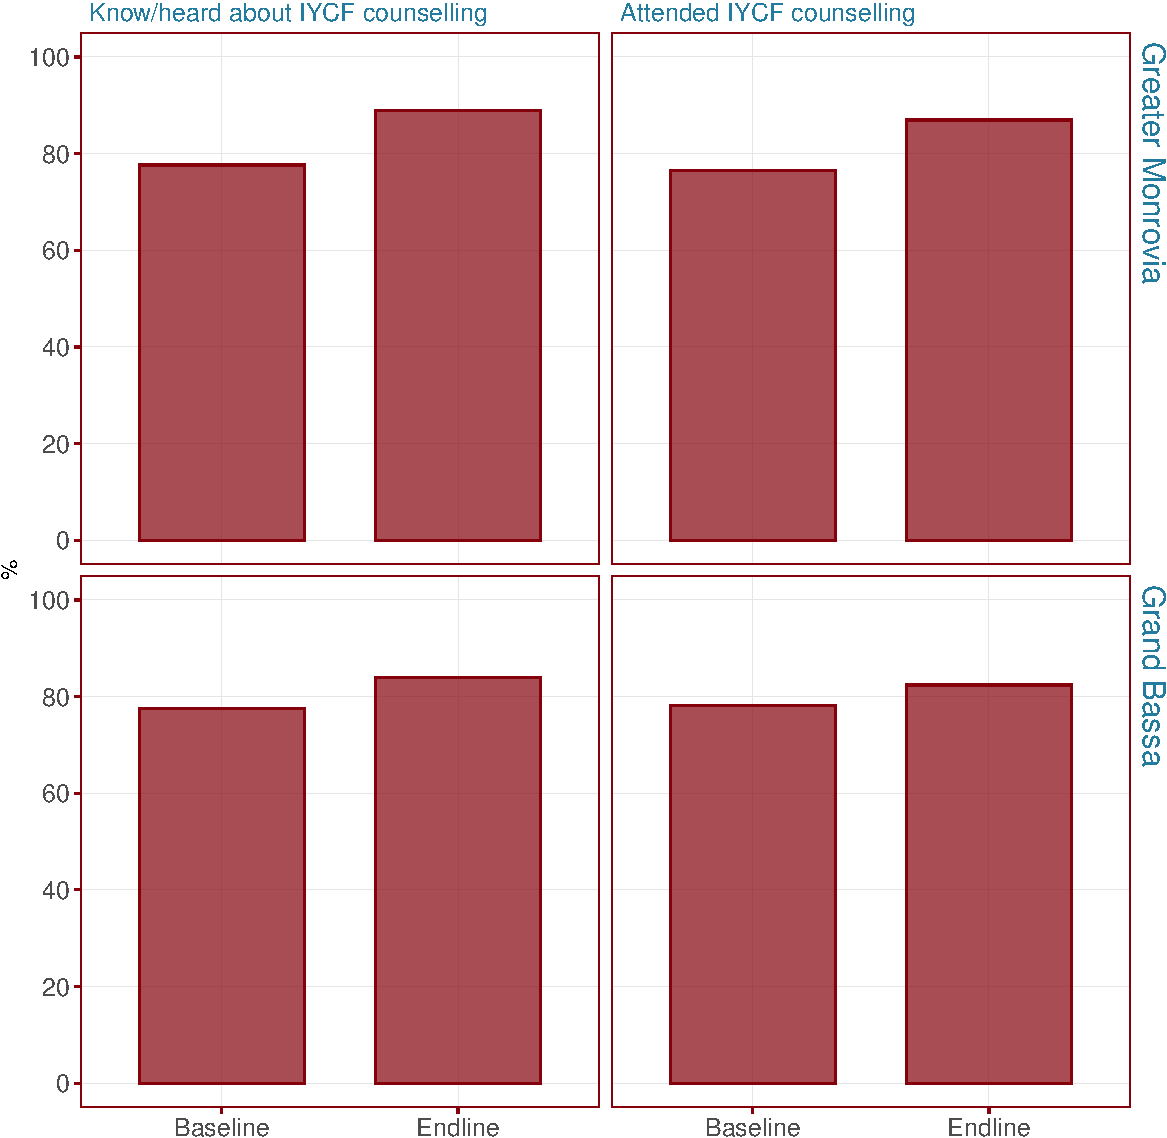
\includegraphics{liberiaCoverageFinalReport_files/figure-latex/icf1plot-1} 

}

\caption{IYCF counselling coverage}\label{fig:icf1plot}
\end{figure}

\begin{table}[H]

\caption{\label{tab:icf1table}IYCF counselling coverage}
\centering
\fontsize{9}{11}\selectfont
\begin{tabular}[t]{l>{\ttfamily}r>{\ttfamily}r>{\ttfamily}r>{\ttfamily}r>{\ttfamily}r>{\ttfamily}r>{\ttfamily}r>{\ttfamily}r>{\ttfamily}r>{\ttfamily}r>{\ttfamily}r>{\ttfamily}r}
\toprule
\multicolumn{1}{c}{\textbf{ }} & \multicolumn{6}{c}{\textbf{Greater Monrovia}} & \multicolumn{6}{c}{\textbf{Grand Bassa}} \\
\cmidrule(l{3pt}r{3pt}){2-7} \cmidrule(l{3pt}r{3pt}){8-13}
\multicolumn{1}{c}{\textbf{ }} & \multicolumn{3}{c}{\textbf{Baseline}} & \multicolumn{3}{c}{\textbf{Endline}} & \multicolumn{3}{c}{\textbf{Baseline}} & \multicolumn{3}{c}{\textbf{Endline}} \\
\cmidrule(l{3pt}r{3pt}){2-4} \cmidrule(l{3pt}r{3pt}){5-7} \cmidrule(l{3pt}r{3pt}){8-10} \cmidrule(l{3pt}r{3pt}){11-13}
\textbf{Indicator} & \textbf{\makecell[c]{Est\\(\%)}} & \textbf{\makecell[c]{95\%\\LCL}} & \textbf{\makecell[c]{95\%\\UCL}} & \textbf{\makecell[c]{Est\\(\%)}} & \textbf{\makecell[c]{95\%\\LCL}} & \textbf{\makecell[c]{95\%\\UCL}} & \textbf{\makecell[c]{Est\\(\%)}} & \textbf{\makecell[c]{95\%\\LCL}} & \textbf{\makecell[c]{95\%\\UCL}} & \textbf{\makecell[c]{Est\\(\%)}} & \textbf{\makecell[c]{95\%\\LCL}} & \textbf{\makecell[c]{95\%\\UCL}}\\
\midrule
\rowcolor{gray!6}  Know/heard about IYCF counselling & 77.6 & 69.2 & 85.4 & 88.9 & 84.7 & 92.5 & 77.5 & 72.1 & 83.7 & 83.9 & 76.4 & 89.2\\
Attended IYCF counselling & 76.5 & 66.3 & 83.4 & 87.0 & 81.5 & 91.4 & 78.1 & 71.3 & 83.3 & 82.4 & 74.9 & 87.9\\
\bottomrule
\end{tabular}
\end{table}

\newpage

Of the few who did not attend IYCF counselling, their main reasons for not attending are presented in \ref{fig:icf2table}. At baseline, mothers not covered by IYCF counselling reported being too busy and timing of IYCF counselling as the main reasons for non-coverage. At endline, timing of IYCF counselling was still an issue but interest in IYCF counselling was reported the most.

\begin{figure}[H]

{\centering 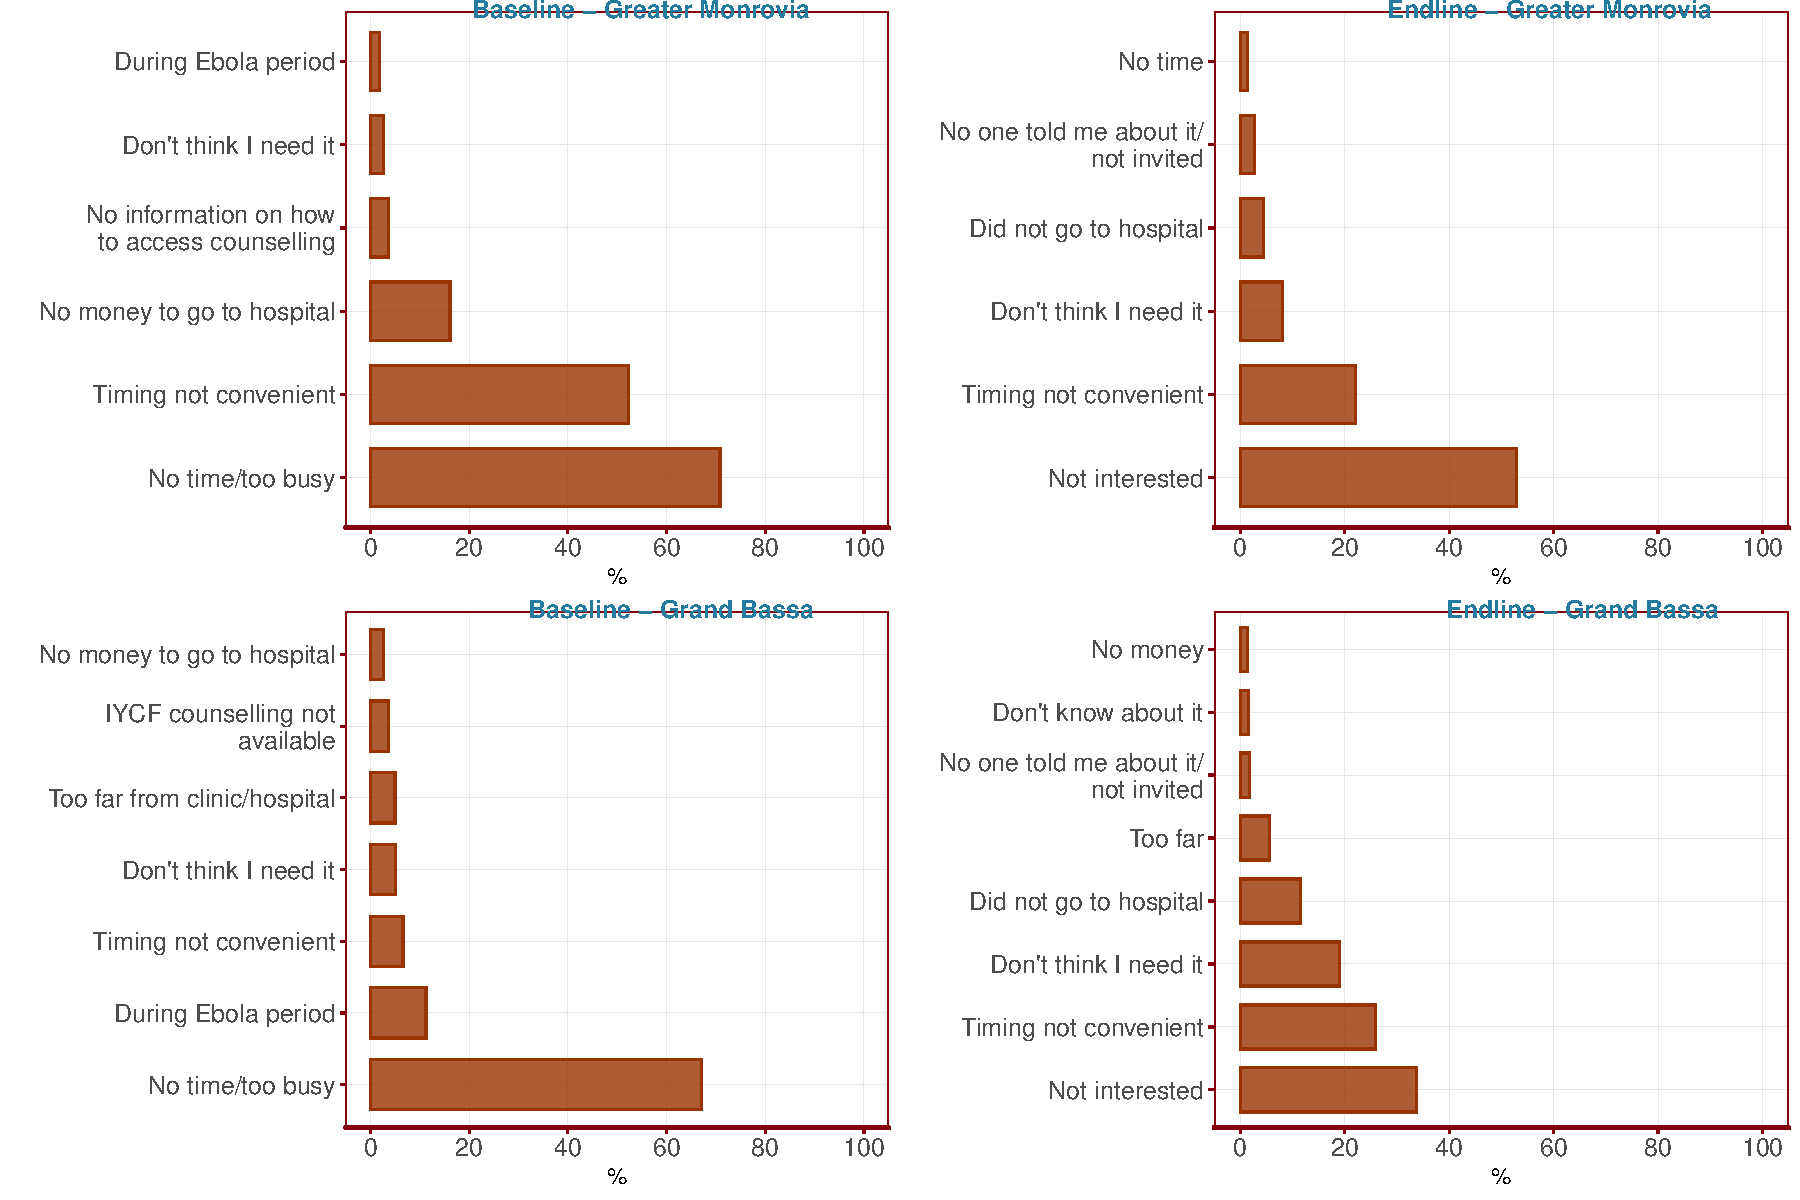
\includegraphics{liberiaCoverageFinalReport_files/figure-latex/icf2table-1} 

}

\caption{Reasons for not attending IYCF counselling}\label{fig:icf2table}
\end{figure}

Spatial distribution of IYCF counselling coverage in Greater Monrovia is shown in Figure \ref{fig:icf1map}. IYCF counselling coverage was at its lowest in eastern sections of Greater Monrovia at baseline. These areas have improved coverage at endline.

Spatial distribution of IYCF counselling coverage in Grand Bassa is shown in Figure \ref{fig:icf2map}. IYCF counselling coverage was at its lowest in southern sections of Grand Bassa at baseline. These areas have improved coverage at endline but with newer focused areas of low coverage spread throughout the county.

\begin{figure}[H]

{\centering 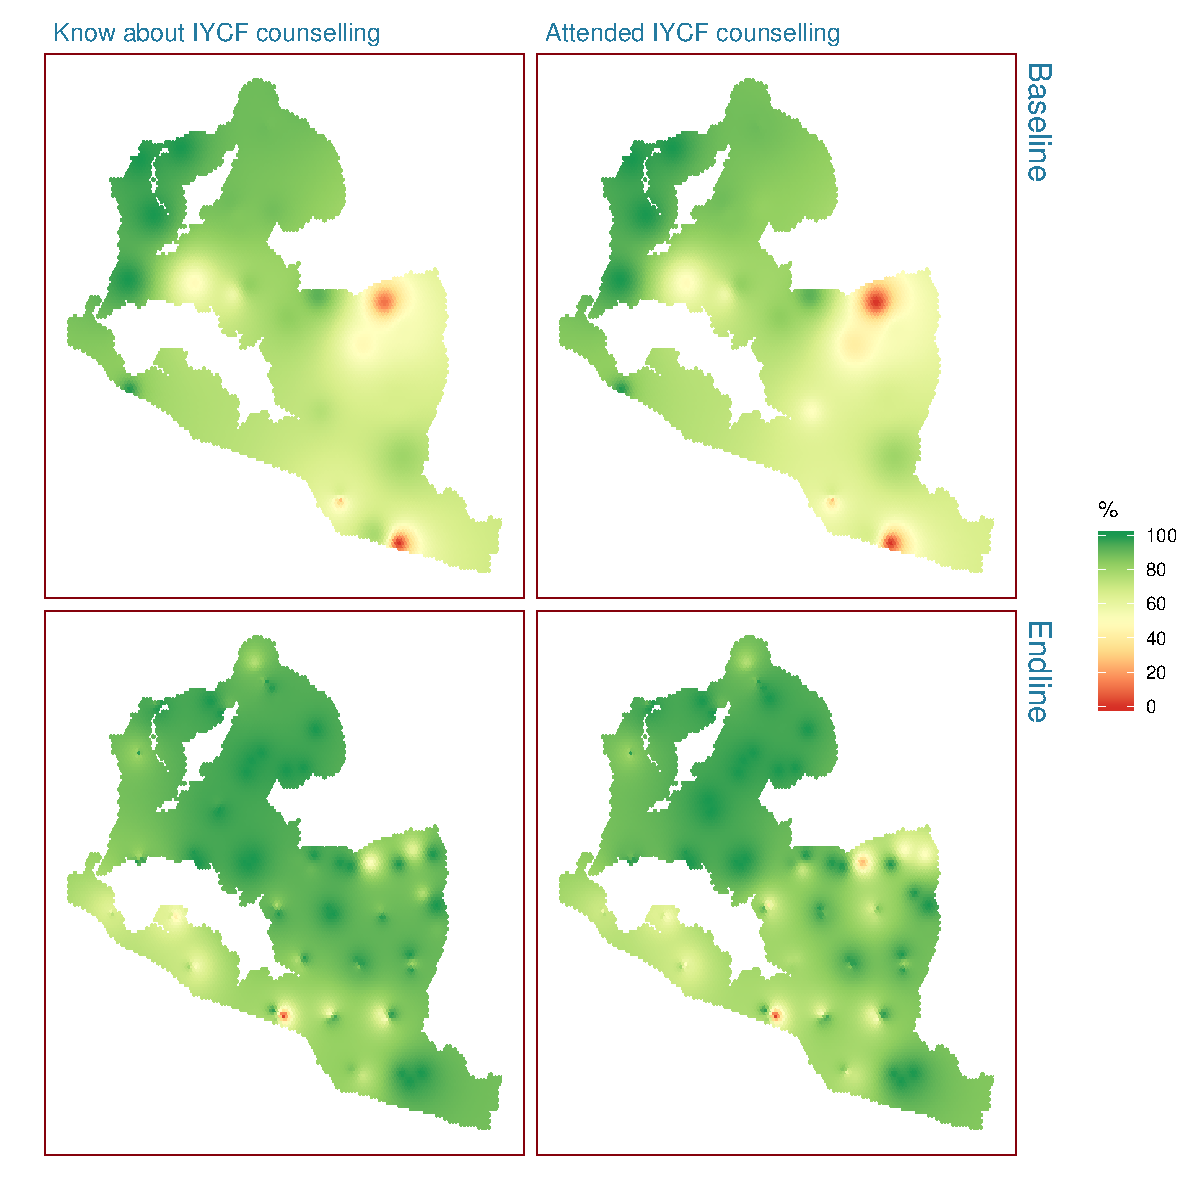
\includegraphics{liberiaCoverageFinalReport_files/figure-latex/icf1map-1} 

}

\caption{Spatial distribution of IYCF counselling coverage in Greater Monrovia}\label{fig:icf1map}
\end{figure}

\begin{figure}[H]

{\centering 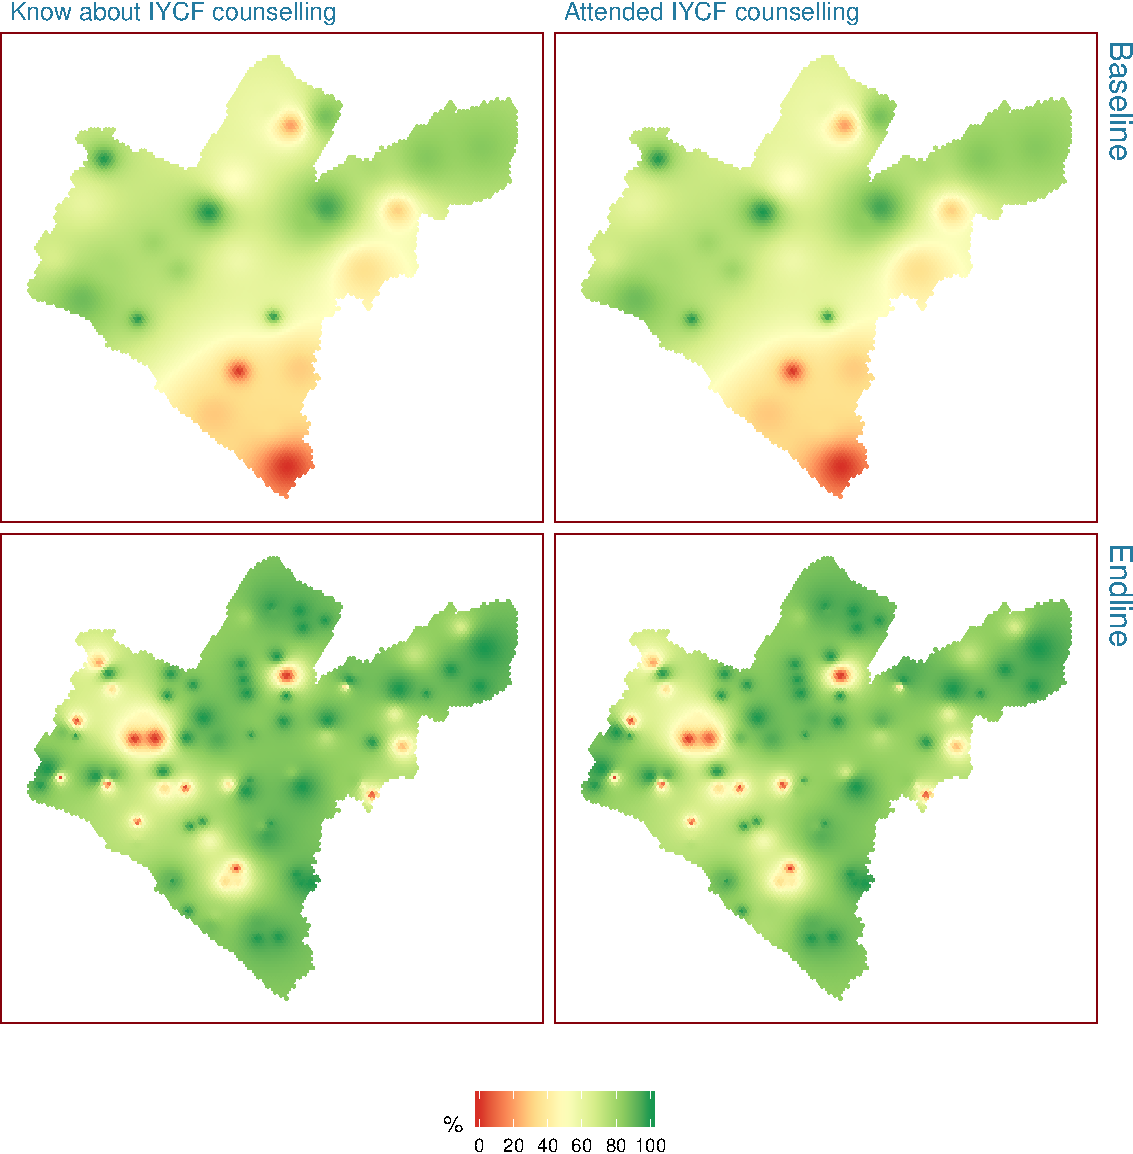
\includegraphics{liberiaCoverageFinalReport_files/figure-latex/icf2map-1} 

}

\caption{Spatial distribution of IYCF counselling coverage in Grand Bassa}\label{fig:icf2map}
\end{figure}

\newpage

\hypertarget{micronutrient-powder-supplementation-coverage}{%
\subsection{Micronutrient powder supplementation coverage}\label{micronutrient-powder-supplementation-coverage}}

Figure \ref{fig:mnp1plot} and Table \ref{tab:mnp1table} summarises the hierarchical MNP supplementation coverage indicators in Greater Monrovia and Grand Bassa. MNP supplementation coverage was extremely low at baseline in each area. This was expected given that programme was at its early implementation phase. At endline, the MNP supplementation coverage indicators have increased significantly compared to baseline with estimates approaching 50\% in both areas. However, it should be noted that these MNP coverage results are still considerably low. From a hierarchical coverage perspective, these results still indicate that knowledge and information about MNP is the key faltering point of the programme.

\begin{figure}[H]

{\centering 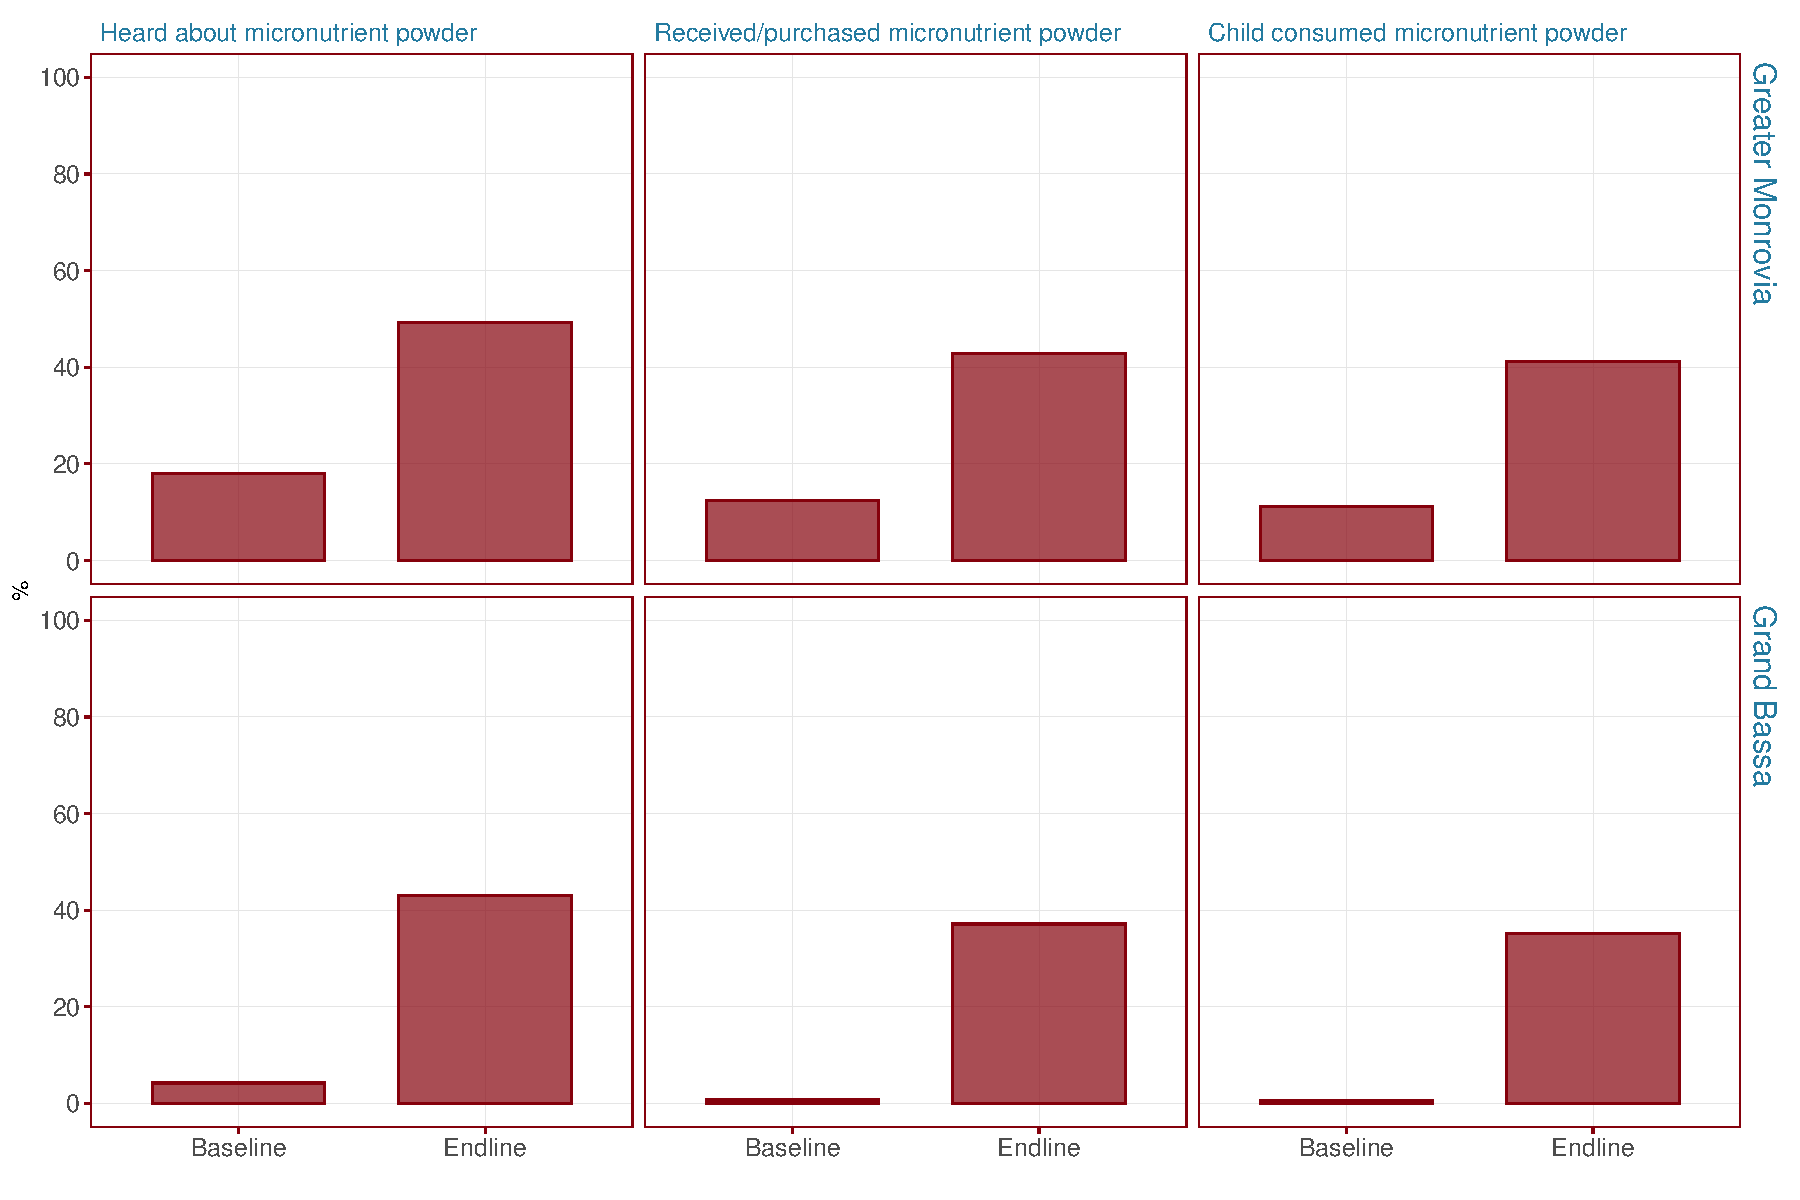
\includegraphics{liberiaCoverageFinalReport_files/figure-latex/mnp1plot-1} 

}

\caption{Micronutrient powder supplementation coverage}\label{fig:mnp1plot}
\end{figure}

\begin{table}[H]

\caption{\label{tab:mnp1table}MNP supplementation coverage}
\centering
\fontsize{9}{11}\selectfont
\begin{tabular}[t]{l>{\ttfamily}r>{\ttfamily}r>{\ttfamily}r>{\ttfamily}r>{\ttfamily}r>{\ttfamily}r>{\ttfamily}r>{\ttfamily}r>{\ttfamily}r>{\ttfamily}r>{\ttfamily}r>{\ttfamily}r}
\toprule
\multicolumn{1}{c}{\textbf{ }} & \multicolumn{6}{c}{\textbf{Greater Monrovia}} & \multicolumn{6}{c}{\textbf{Grand Bassa}} \\
\cmidrule(l{3pt}r{3pt}){2-7} \cmidrule(l{3pt}r{3pt}){8-13}
\multicolumn{1}{c}{\textbf{ }} & \multicolumn{3}{c}{\textbf{Baseline}} & \multicolumn{3}{c}{\textbf{Endline}} & \multicolumn{3}{c}{\textbf{Baseline}} & \multicolumn{3}{c}{\textbf{Endline}} \\
\cmidrule(l{3pt}r{3pt}){2-4} \cmidrule(l{3pt}r{3pt}){5-7} \cmidrule(l{3pt}r{3pt}){8-10} \cmidrule(l{3pt}r{3pt}){11-13}
\textbf{Indicator} & \textbf{\makecell[c]{Est\\(\%)}} & \textbf{\makecell[c]{95\%\\LCL}} & \textbf{\makecell[c]{95\%\\UCL}} & \textbf{\makecell[c]{Est\\(\%)}} & \textbf{\makecell[c]{95\%\\LCL}} & \textbf{\makecell[c]{95\%\\UCL}} & \textbf{\makecell[c]{Est\\(\%)}} & \textbf{\makecell[c]{95\%\\LCL}} & \textbf{\makecell[c]{95\%\\UCL}} & \textbf{\makecell[c]{Est\\(\%)}} & \textbf{\makecell[c]{95\%\\LCL}} & \textbf{\makecell[c]{95\%\\UCL}}\\
\midrule
\rowcolor{gray!6}  Heard about micronutrient powder & 17.9 & 10.5 & 26.5 & 49.3 & 38.4 & 59.9 & 4.2 & 0.8 & 9.0 & 43.1 & 29.8 & 55.0\\
Received/purchased micronutrient powder & 12.5 & 5.7 & 20.8 & 42.8 & 31.1 & 54.2 & 0.7 & 0.0 & 3.4 & 37.1 & 25.9 & 48.4\\
\rowcolor{gray!6}  Child consumed micronutrient powder & 11.1 & 3.9 & 19.4 & 41.2 & 29.4 & 52.4 & 0.7 & 0.0 & 3.0 & 35.2 & 24.9 & 47.2\\
\bottomrule
\end{tabular}
\end{table}

The main reasons for not receiving MNP supplements are presented in Figure \ref{fig:mnp2plot}. At baseline, availability of MNP was the main reason for non-coverage. At endline, reasons have shifted more to personal preferences by parents not to have children take the MNP supplement mainly because they think their child doesn't need the supplement. It should be noted, however, that given the coverage results, knowledge, awareness and information about MNP supplementation is the main falter point for coverage and this is reflected in the various reasons conveyed by those not covered.

\begin{figure}[H]

{\centering 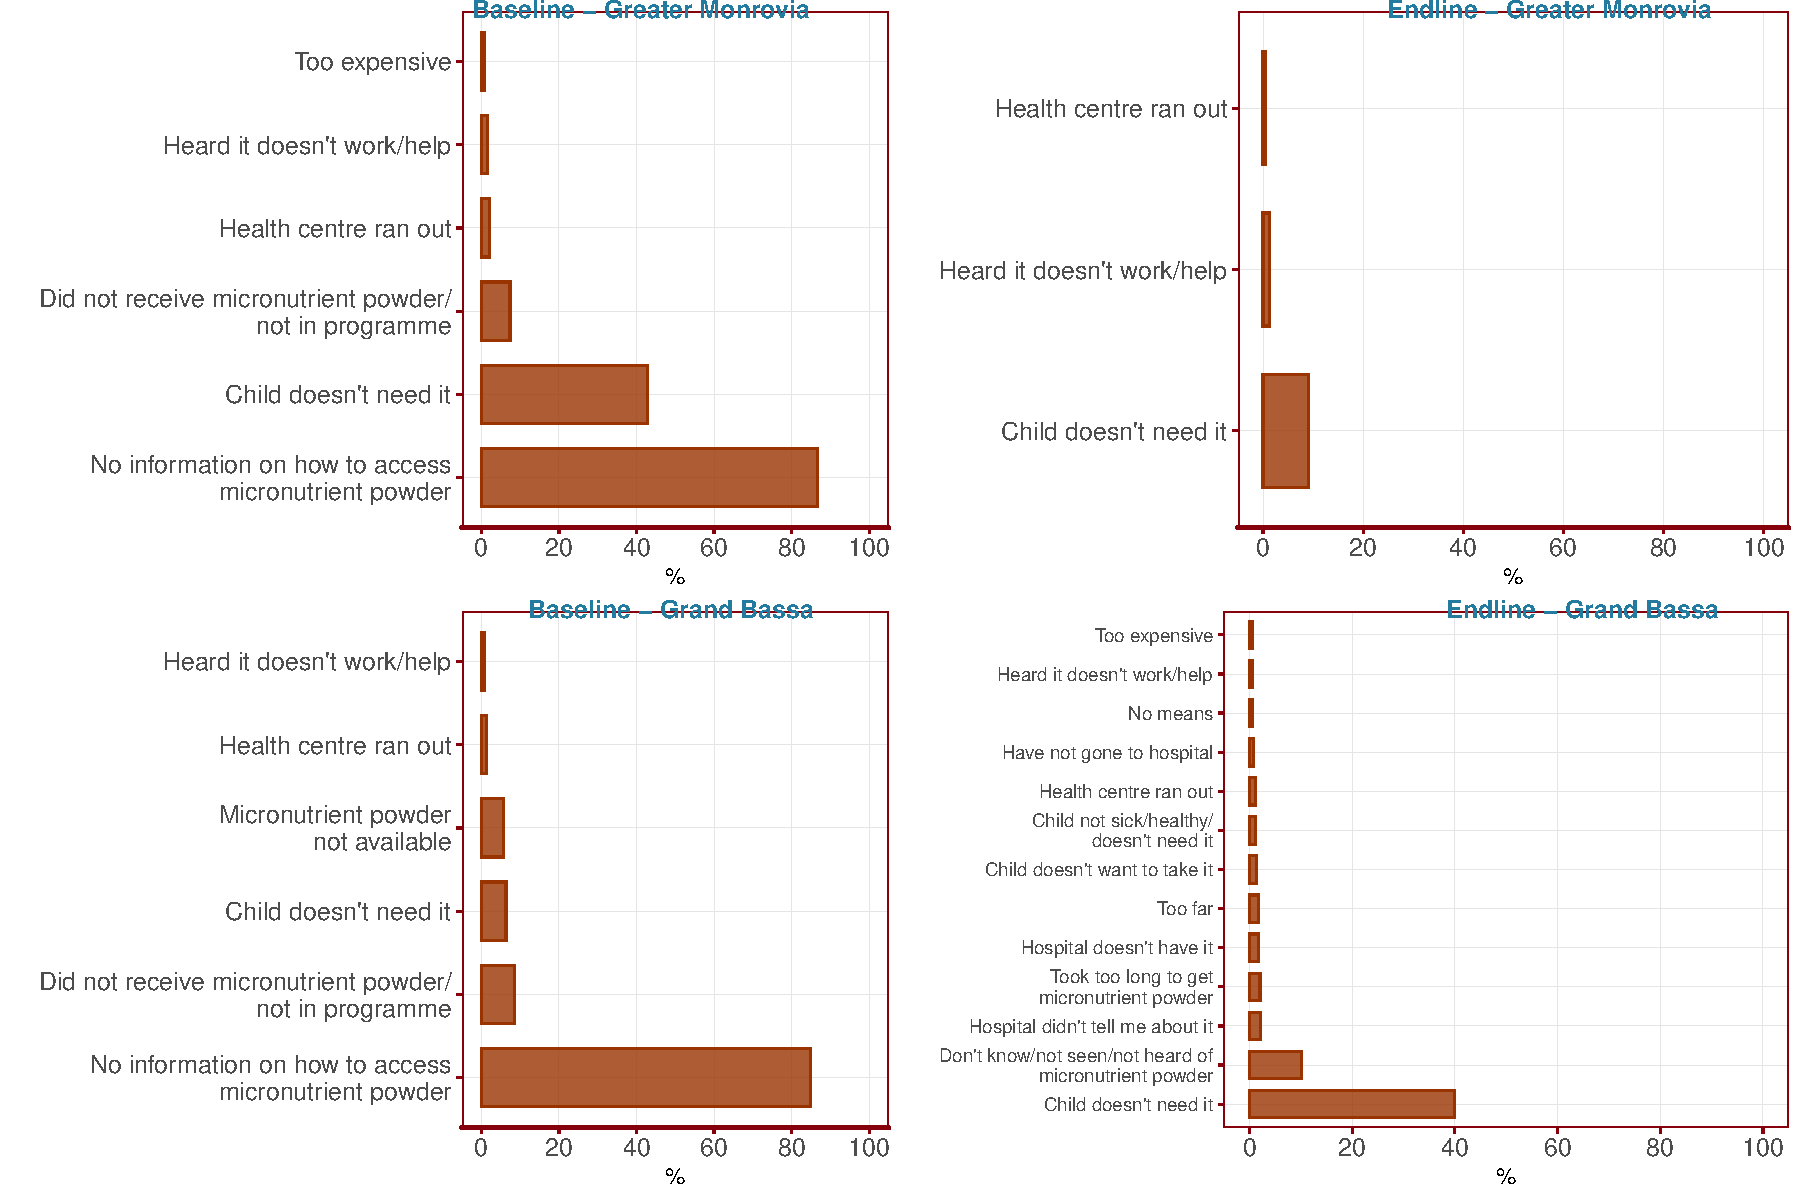
\includegraphics{liberiaCoverageFinalReport_files/figure-latex/mnp2plot-1} 

}

\caption{Reasons for not receiving micronutrient powder}\label{fig:mnp2plot}
\end{figure}

Spatial distribution of MNP supplementation coverage was all throughout low in Greater Monrovia and Grand Bassa at baseline. By endline, improved coverage was concentrated in the north and central areas of Greater Monrovia (see Figure \ref{fig:mnp1map}) and at north and central areas of Grand Bassa (see Figure \ref{fig:mnp2map}). The spatial distribution of coverage for both areas emphasise the point that despite increased aggregated coverage shown above, a still greater number of children and areas are uncovered by the MNP supplementation programme.

\begin{figure}[H]

{\centering 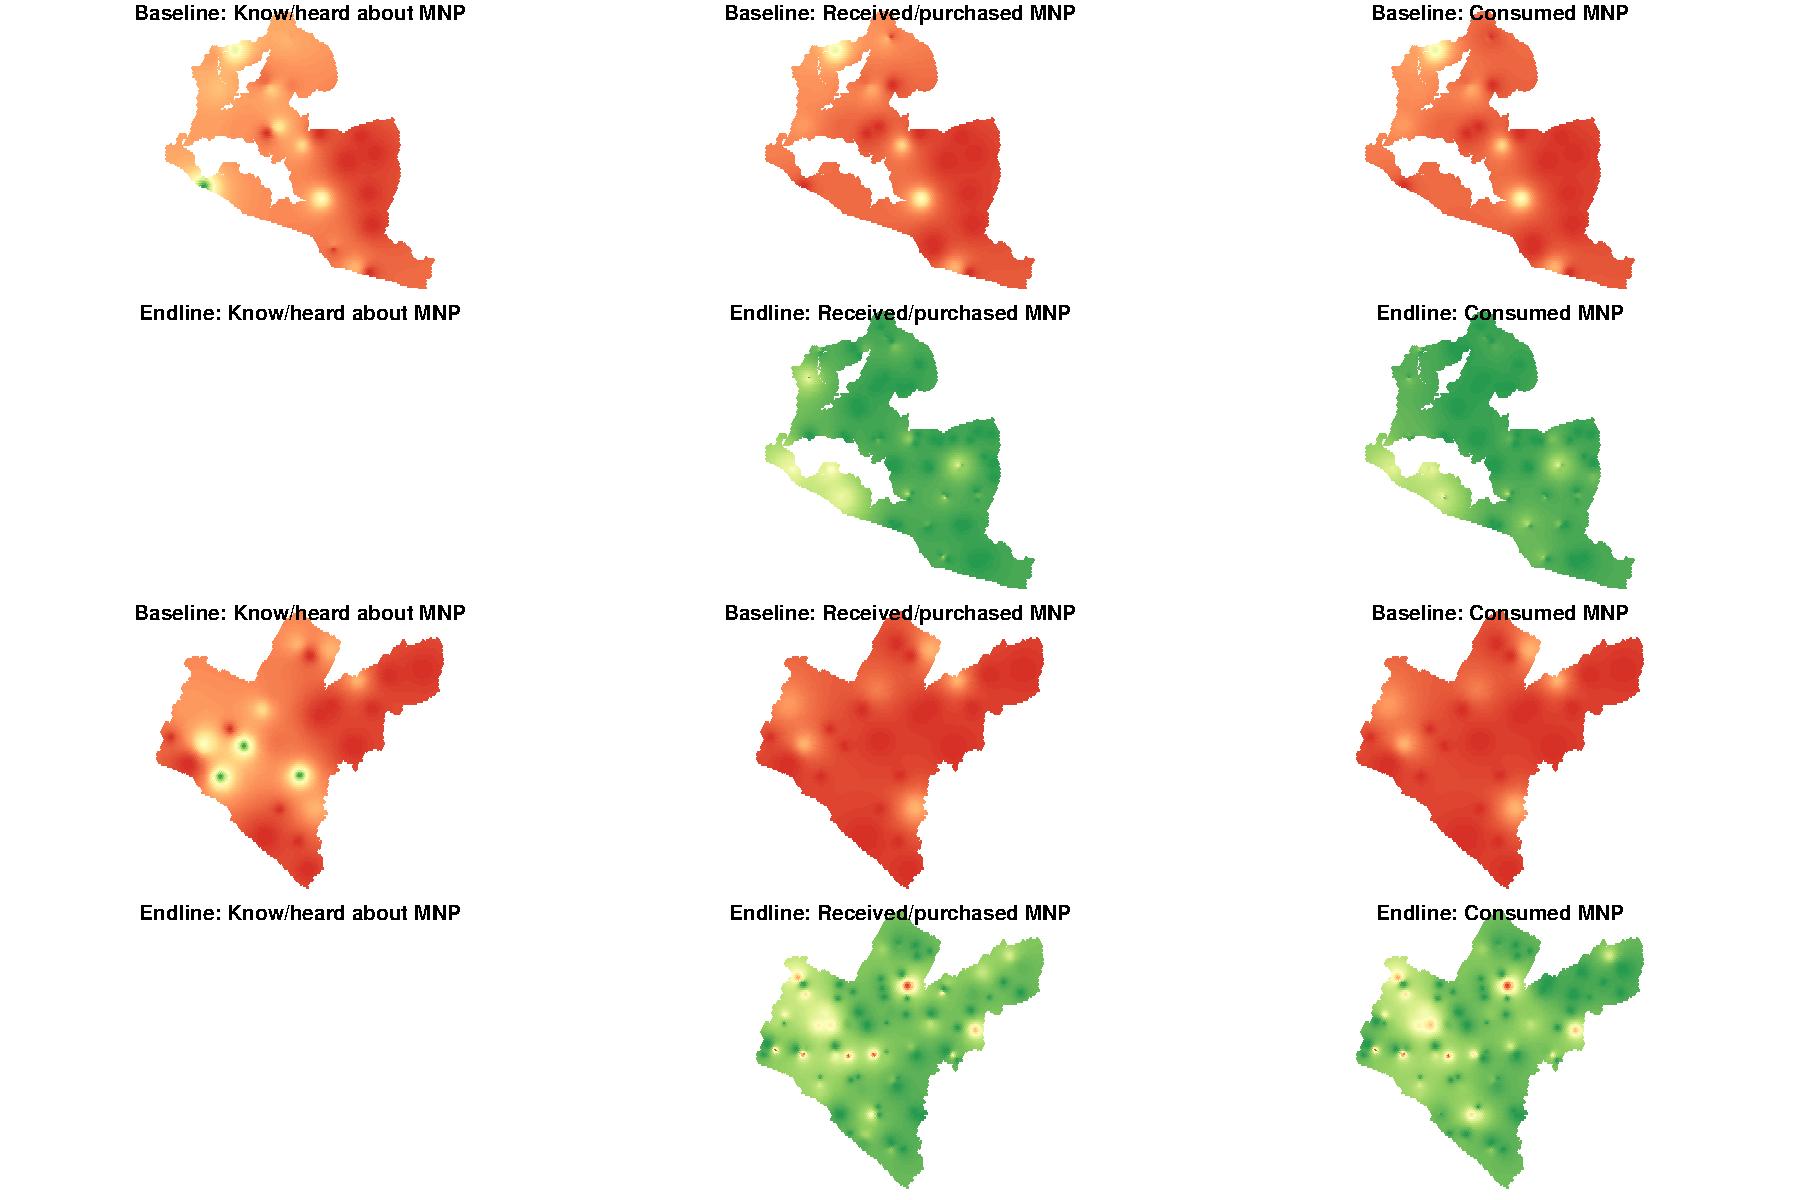
\includegraphics{liberiaCoverageFinalReport_files/figure-latex/mnp1map-1} 

}

\caption{Spatial distribution of MNP supplementation coverage in Greater Monrovia}\label{fig:mnp1map}
\end{figure}

\begin{figure}[H]

{\centering 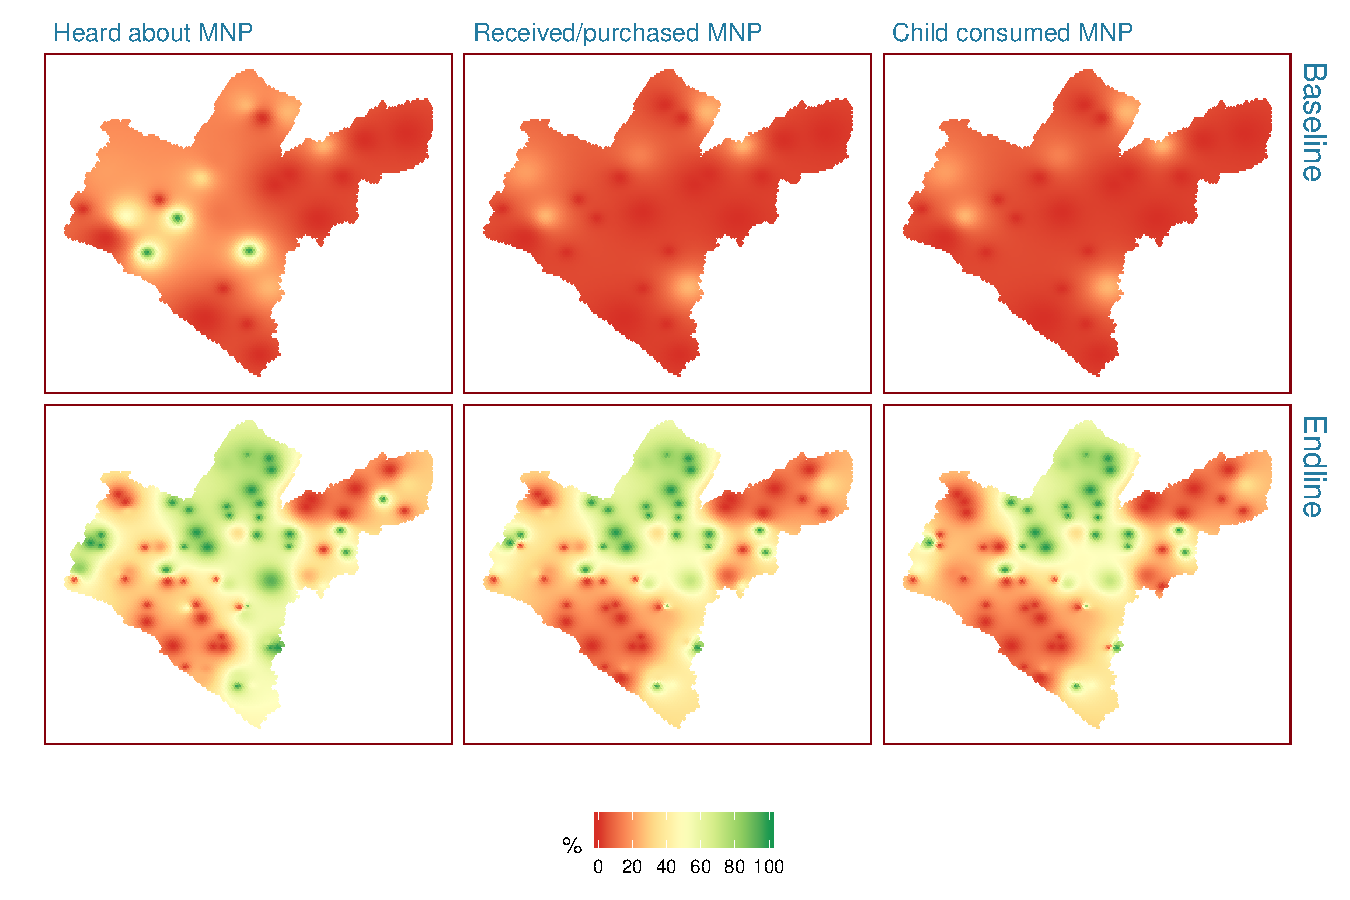
\includegraphics{liberiaCoverageFinalReport_files/figure-latex/mnp2map-1} 

}

\caption{Spatial distribution of MNP supplementation coverage in Grand Bassa}\label{fig:mnp2map}
\end{figure}

\newpage

\hypertarget{vitamin-a-supplementation-coverage}{%
\subsection{Vitamin A Supplementation Coverage}\label{vitamin-a-supplementation-coverage}}

Vitamin A supplementation coverage in Greater Monrovia and Grand Bassa is shown in Figure \ref{fig:vit1plot}. There were 82\% of children 6-59 months in Greater Monrovia who received vitamin A supplementation in the past 6 months at baseline. This rate dropped slightly at endline to 78\% though this difference is not statistically significant. In Grand Bassa, about 84\% of children 6-59 months received vitamin A supplementation in the past 6 months at baseline. This dropped slightly to about 82\% at endline though the difference is not statistically significant.

\begin{figure}[H]

{\centering 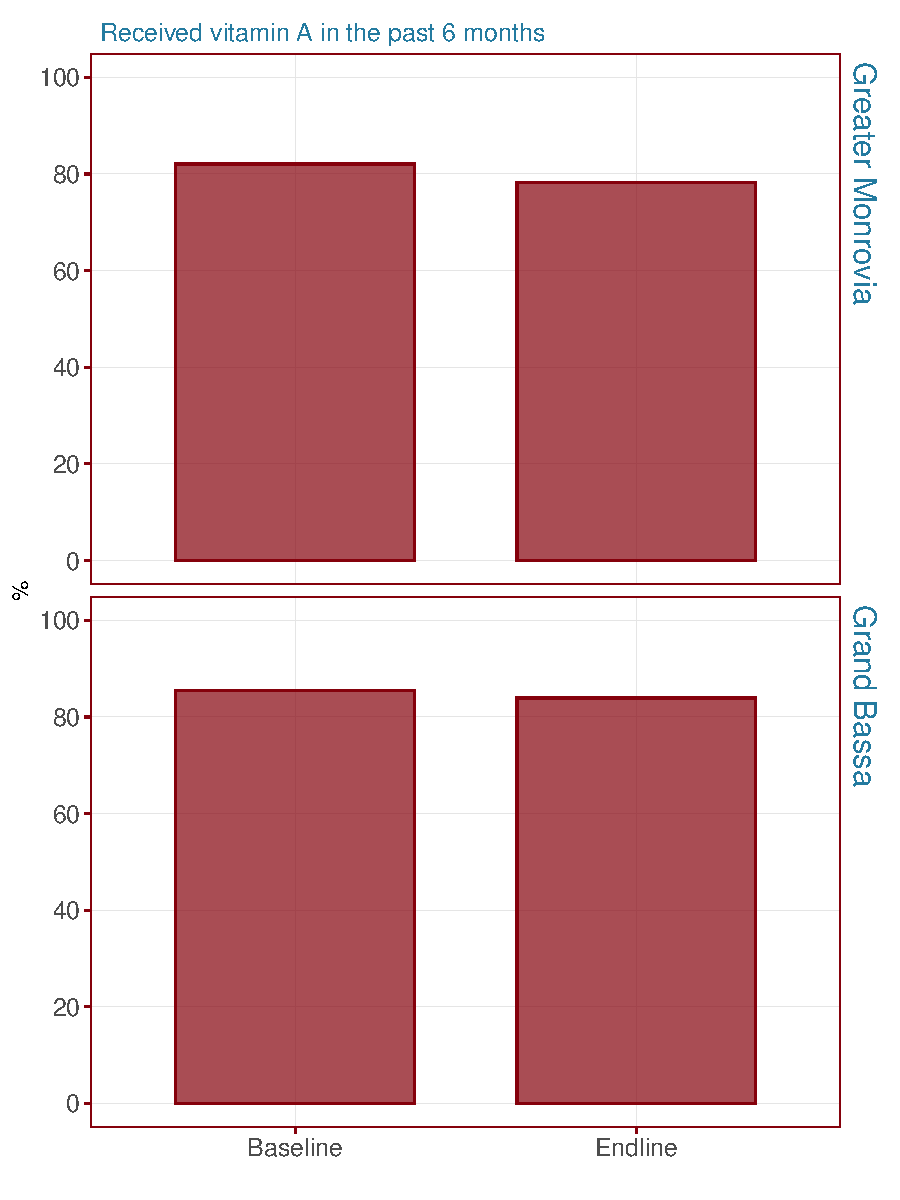
\includegraphics{liberiaCoverageFinalReport_files/figure-latex/vit1plot-1} 

}

\caption{Vitamin A supplementation coverage}\label{fig:vit1plot}
\end{figure}

Spatial distribution of vitamin A supplementation in Greater Monrovia is shown in Figure \ref{fig:vit1map}. The south and eastern areas of Greater Monrovia have the lowest vitamin A supplementation coverage which have shown improvement at endline though other areas in the northeast and southwest of Greater Monrovia have decreased vitamin A supplementation. Spatial distribution of vitamin A supplementation in Grand Bassa is shown in Figure \ref{fig:vit2map}. The south, central and northern areas of Grand Bassa have the lowest vitamin A supplementation coverage which have shown improvement at endline though other areas in the southeast and northeast of Grand Bassa have decreased vitamin A supplementation.

\begin{figure}[H]

{\centering 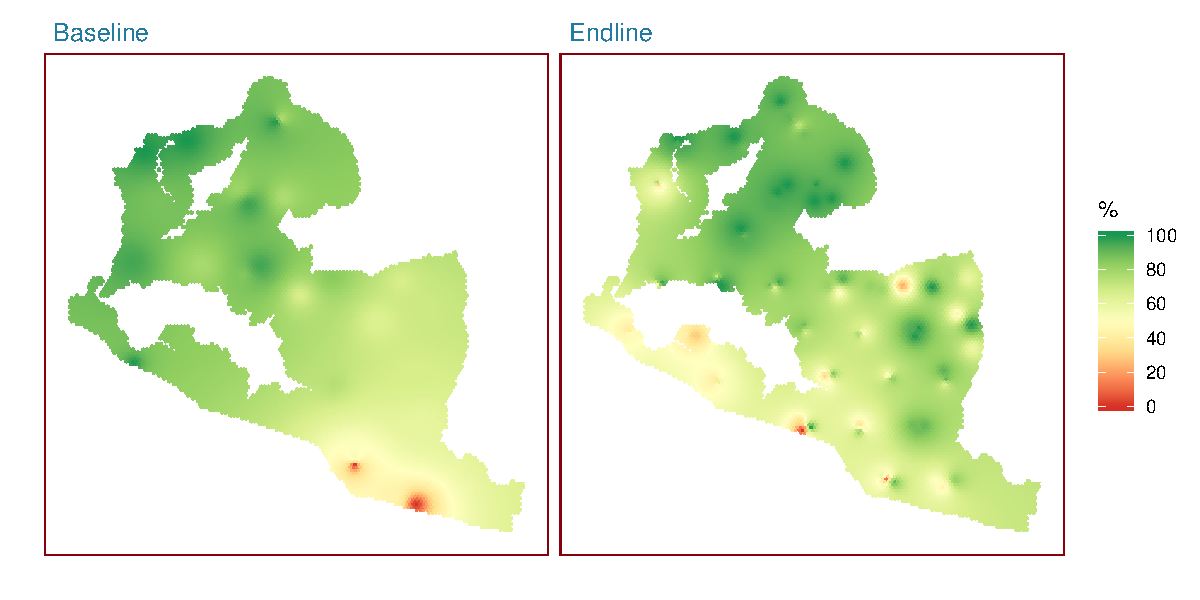
\includegraphics{liberiaCoverageFinalReport_files/figure-latex/vit1map-1} 

}

\caption{Spatial distribution of vitamin A coverage in Greater Monrovia}\label{fig:vit1map}
\end{figure}

\begin{figure}[H]

{\centering 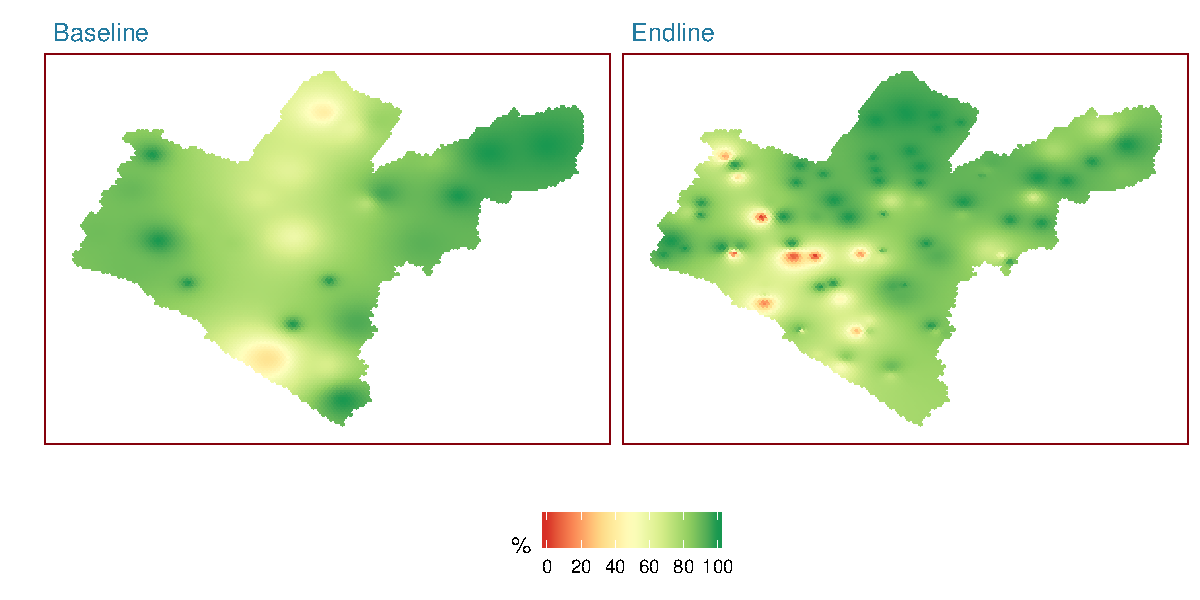
\includegraphics{liberiaCoverageFinalReport_files/figure-latex/vit2map-1} 

}

\caption{Spatial distribution of vitamin A coverage in Grand Bassa}\label{fig:vit2map}
\end{figure}

The main reasons for not receiving vitamin A are presented in Figure \ref{fig:vit2plot}. At baseline, the main reasons for non-coverage was access and availability of the supplement. At endline, these reasons are still the most common in Grand Bassa but for Greater Monrovia, there is a factor of mothers choosing not to have their children receive the supplement as they perceive their child not needing it.

\begin{figure}[H]

{\centering 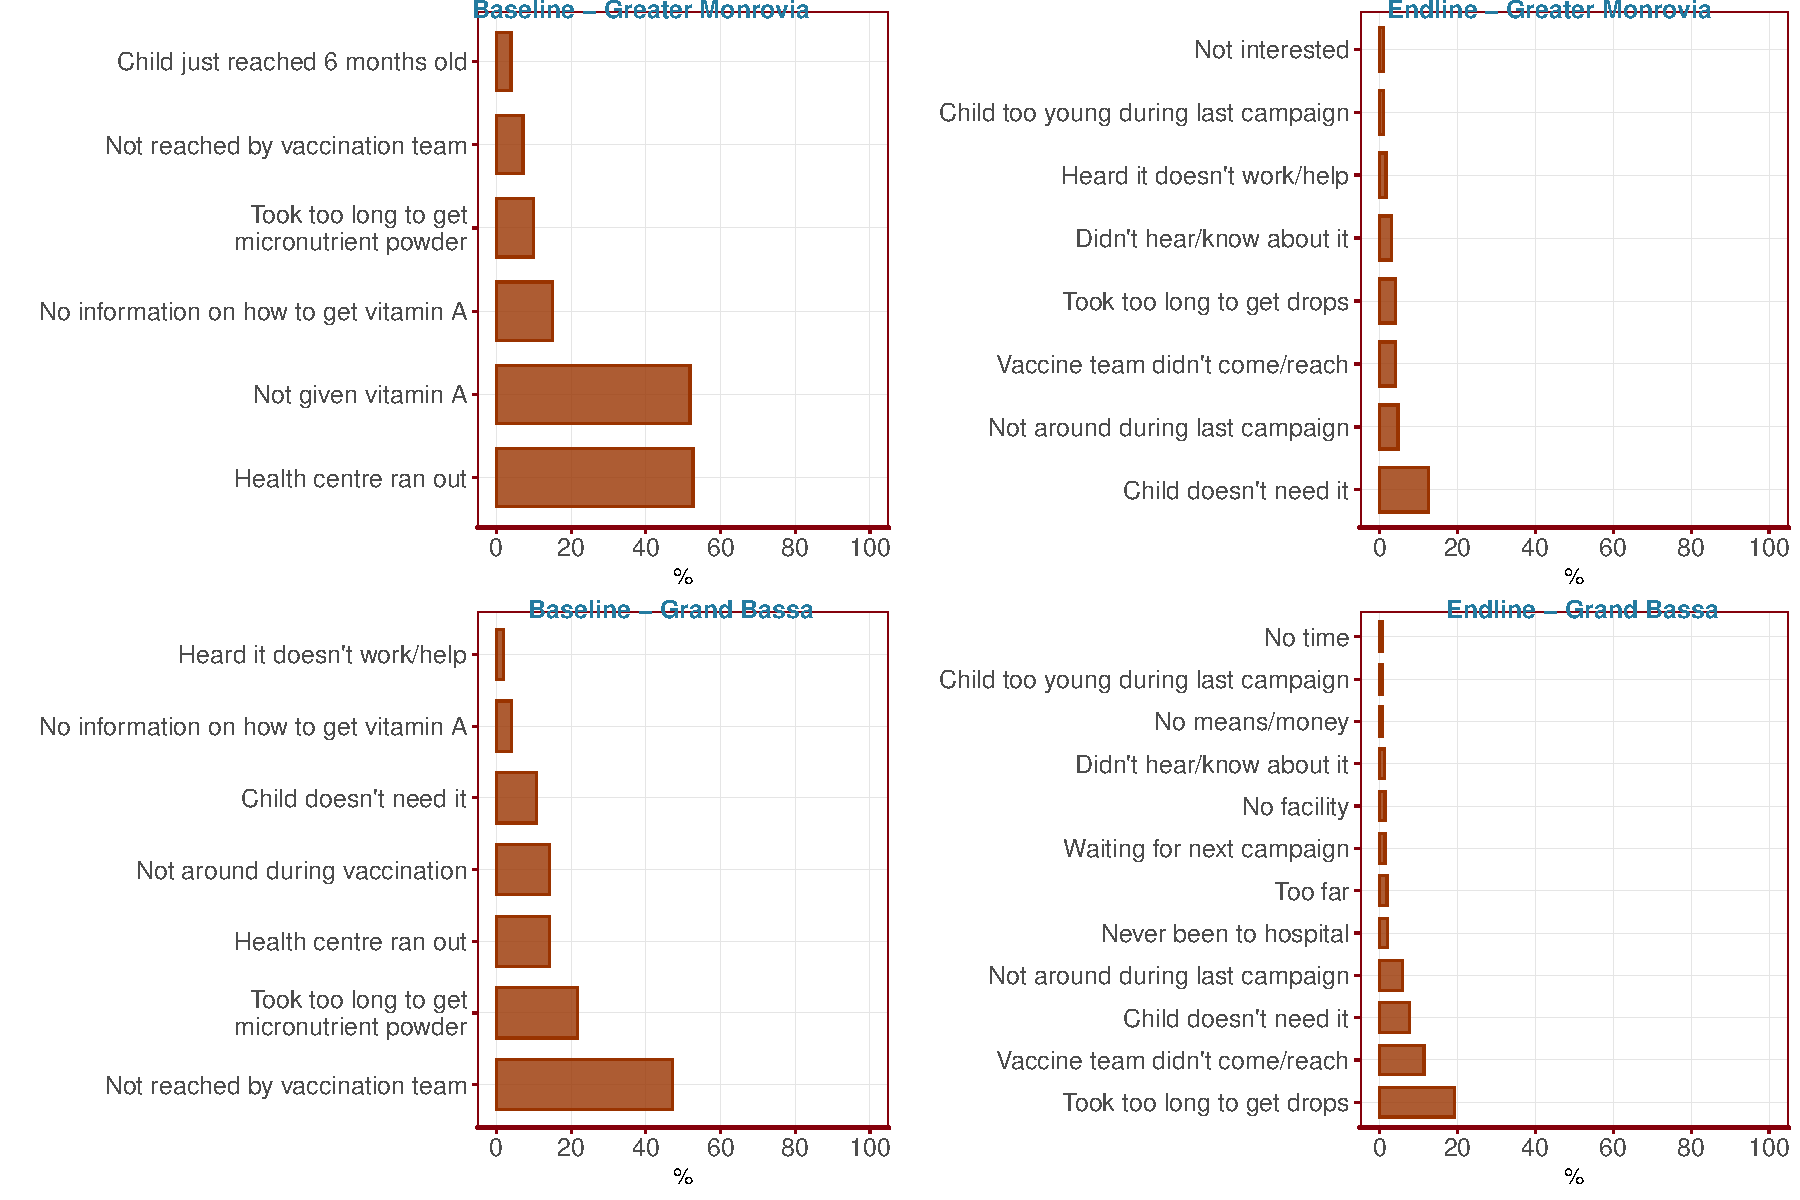
\includegraphics{liberiaCoverageFinalReport_files/figure-latex/vit2plot-1} 

}

\caption{Reasons for not receiving vitamin A}\label{fig:vit2plot}
\end{figure}

\newpage

\hypertarget{stuntingstuntedness-prevalence}{%
\subsection{Stunting/stuntedness prevalence}\label{stuntingstuntedness-prevalence}}

At endline, weight and height measurements were also measured. This allowed for prevalence of stunting/stuntedness to be assessed as presented in Figure \ref{fig:stunt1plot} and Table \ref{tab:stunt1table}. Global stunting/stuntedness is at 22\% in Greater Monrovia of which about 15\% are children with moderate stunting/stuntedness and about 8\% severe. In Grand Bassa, global stunting/stuntedness is significantly higher at a little over 44\%, 24\% of which are children with moderate stunting/stuntedness and about 20\% severe.

\begin{figure}[H]

{\centering 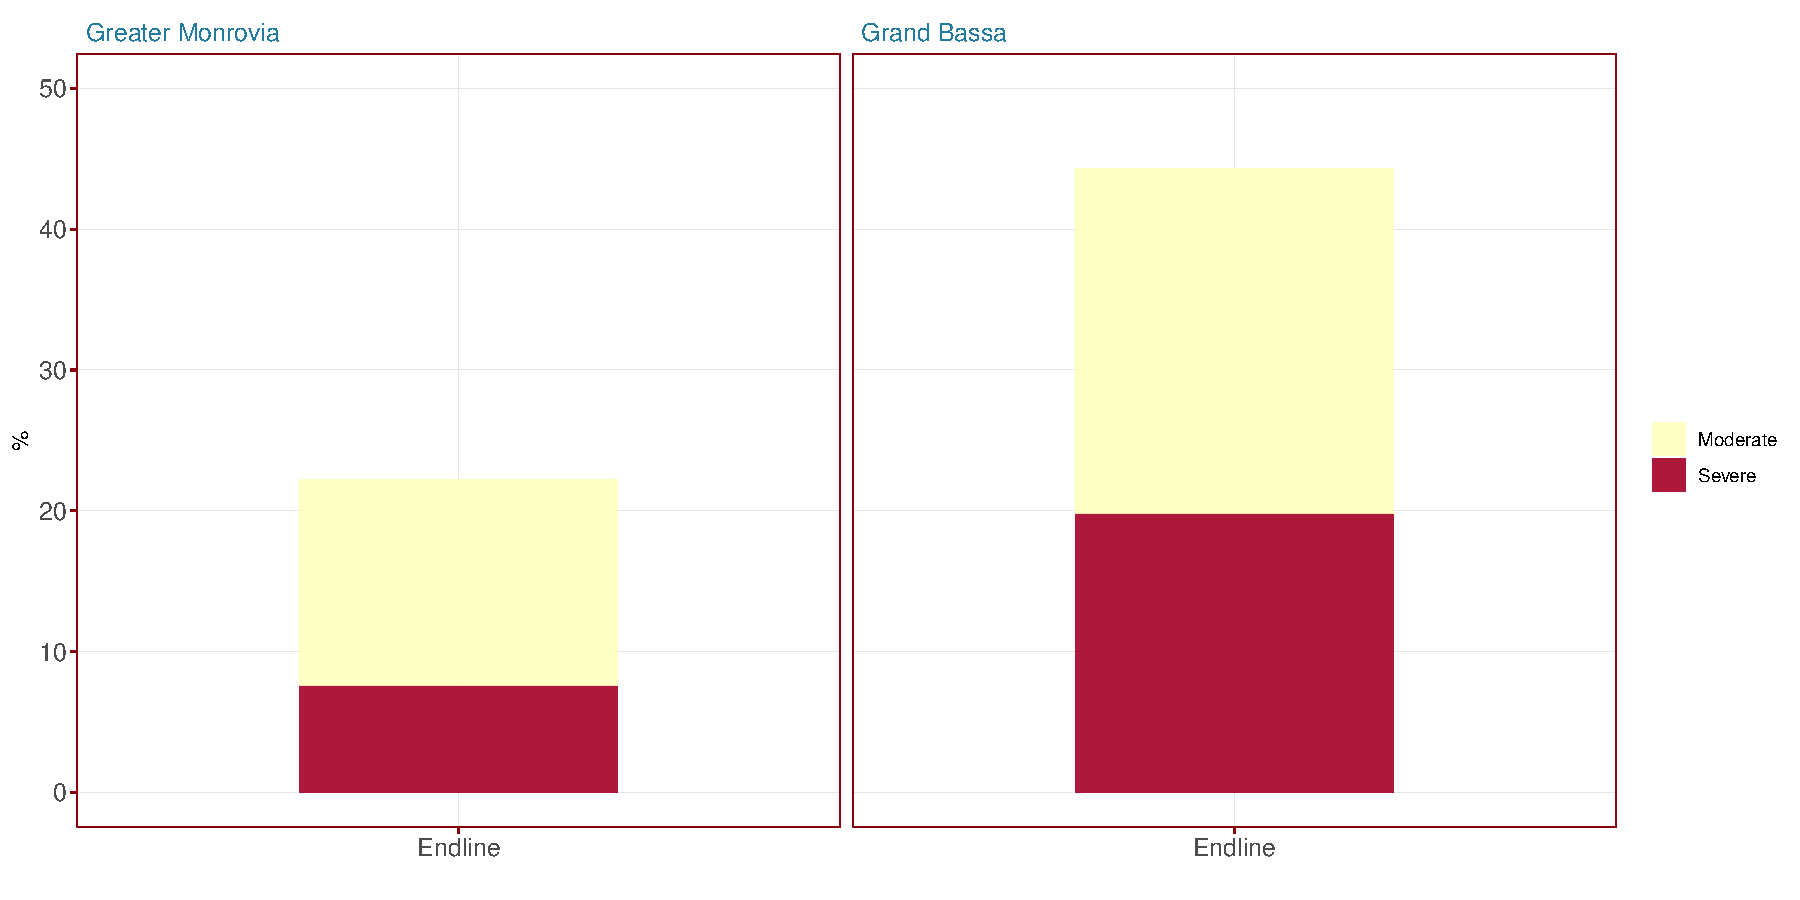
\includegraphics{liberiaCoverageFinalReport_files/figure-latex/stunt1plot-1} 

}

\caption{Stunting/stuntedness prevalence}\label{fig:stunt1plot}
\end{figure}

\begin{table}[H]

\caption{\label{tab:stunt1table}Stunting/stuntedness prevalence}
\centering
\fontsize{9}{11}\selectfont
\begin{tabular}[t]{lrrrrrr}
\toprule
\multicolumn{1}{c}{ } & \multicolumn{3}{c}{Greater Monrovia} & \multicolumn{3}{c}{Grand Bassa} \\
\cmidrule(l{3pt}r{3pt}){2-4} \cmidrule(l{3pt}r{3pt}){5-7}
\textbf{Indicator} & \textbf{\makecell[c]{Est\\(\%)}} & \textbf{\makecell[c]{95\%\\LCL}} & \textbf{\makecell[c]{95\%\\UCL}} & \textbf{\makecell[c]{Est\\(\%)}} & \textbf{\makecell[c]{95\%\\LCL}} & \textbf{\makecell[c]{95\%\\UCL}}\\
\midrule
\rowcolor{gray!6}  Global stunting/stuntedness & 22.2 & 20.3 & 24.4 & 44.3 & 41.6 & 47.5\\
Moderate stunting/stuntedness & 14.6 & 12.8 & 16.6 & 24.4 & 21.8 & 27.1\\
\rowcolor{gray!6}  Severe stunting/stuntedness & 7.6 & 6.4 & 9.0 & 19.8 & 17.9 & 22.2\\
\bottomrule
\end{tabular}
\end{table}

\newpage

\hypertarget{acute-undernutrition-prevalence-by-muac}{%
\subsection{Acute undernutrition prevalence by MUAC}\label{acute-undernutrition-prevalence-by-muac}}

Prevalence of acute undernutrition is presented in Figure \ref{fig:nut1plot} and Table \ref{tab:nut1table}. Acute undernutrition rates were highest in Grand Bassa reaching up to 4\% GAM and close to 2\% GAM in Greater Monrovia at baseline. These estimates are relatively low but are the generally expected values for these areas in Liberia. At endline, the rates for Greater Monrovia increased slightly while for Grand Bassa they decreased slightly. These changes are not statistically significant.

\begin{figure}[H]

{\centering 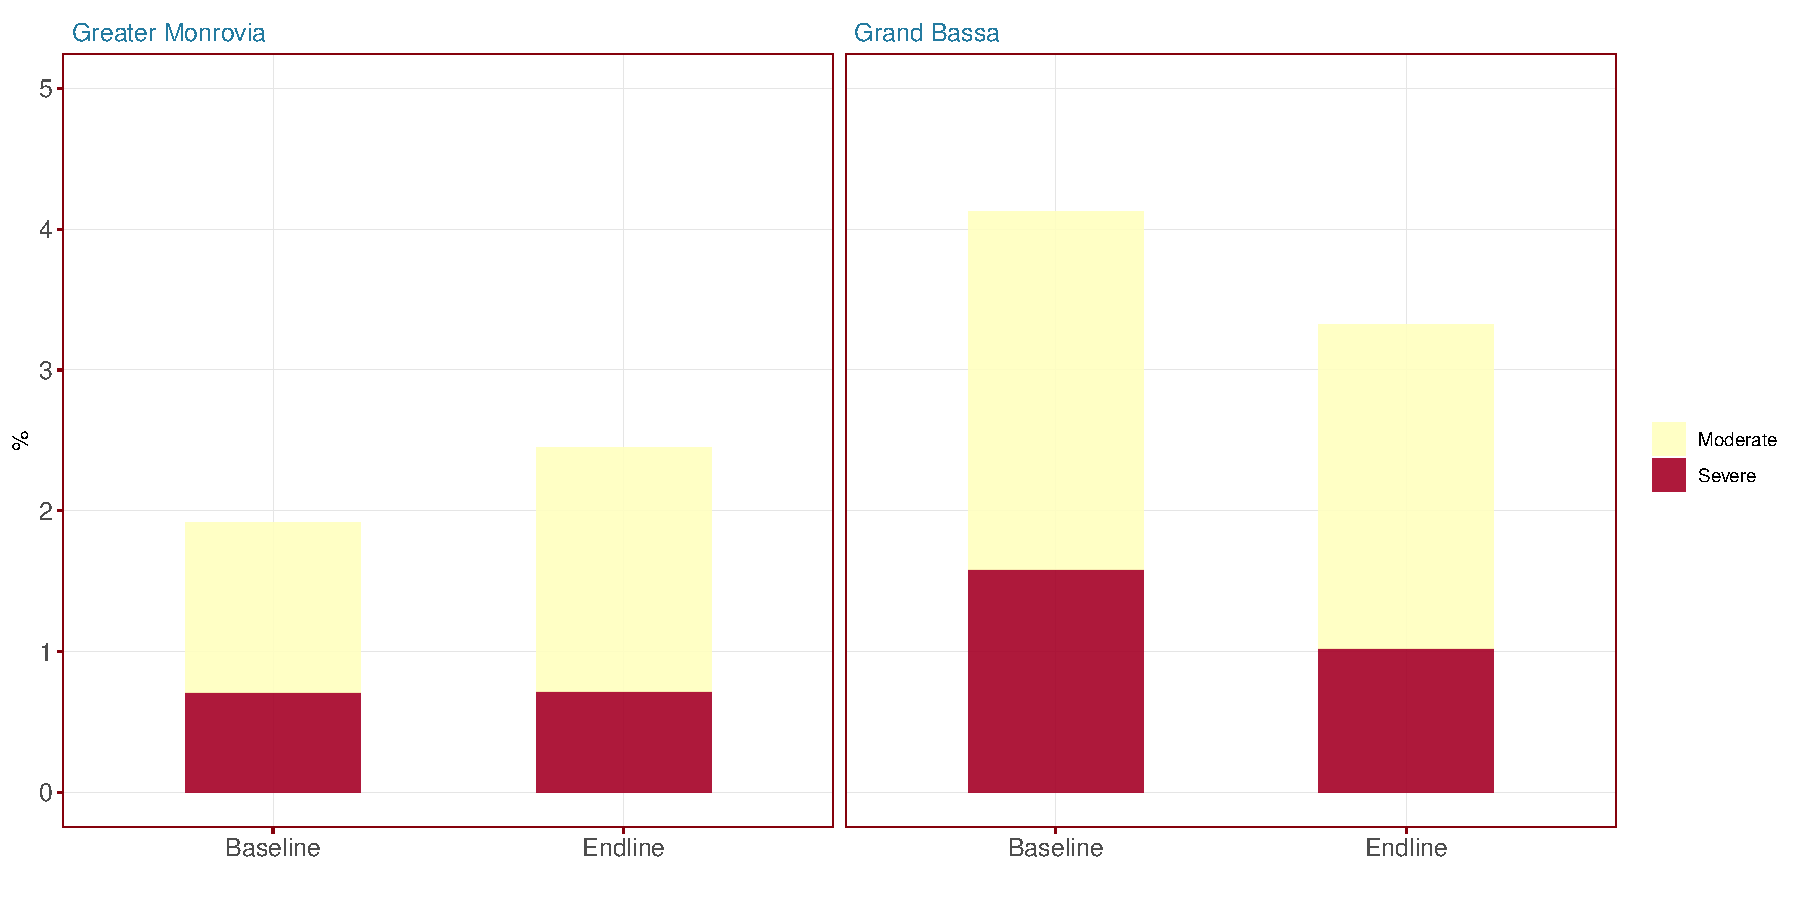
\includegraphics{liberiaCoverageFinalReport_files/figure-latex/nut1plot-1} 

}

\caption{Acute undernutrition prevalence}\label{fig:nut1plot}
\end{figure}

\begin{table}[H]

\caption{\label{tab:nut1table}Acute undernutrition by MUAC prevalence}
\centering
\fontsize{9}{11}\selectfont
\begin{tabular}[t]{lrrrrrrrrrrrr}
\toprule
\multicolumn{1}{c}{ } & \multicolumn{6}{c}{Greater Monrovia} & \multicolumn{6}{c}{Grand Bassa} \\
\cmidrule(l{3pt}r{3pt}){2-7} \cmidrule(l{3pt}r{3pt}){8-13}
\multicolumn{1}{c}{\textbf{ }} & \multicolumn{3}{c}{\textbf{Baseline}} & \multicolumn{3}{c}{\textbf{Endline}} & \multicolumn{3}{c}{\textbf{Baseline}} & \multicolumn{3}{c}{\textbf{Endline}} \\
\cmidrule(l{3pt}r{3pt}){2-4} \cmidrule(l{3pt}r{3pt}){5-7} \cmidrule(l{3pt}r{3pt}){8-10} \cmidrule(l{3pt}r{3pt}){11-13}
\textbf{Indicator} & \textbf{\makecell[c]{Est\\(\%)}} & \textbf{\makecell[c]{95\%\\LCL}} & \textbf{\makecell[c]{95\%\\UCL}} & \textbf{\makecell[c]{Est\\(\%)}} & \textbf{\makecell[c]{95\%\\LCL}} & \textbf{\makecell[c]{95\%\\UCL}} & \textbf{\makecell[c]{Est\\(\%)}} & \textbf{\makecell[c]{95\%\\LCL}} & \textbf{\makecell[c]{95\%\\UCL}} & \textbf{\makecell[c]{Est\\(\%)}} & \textbf{\makecell[c]{95\%\\LCL}} & \textbf{\makecell[c]{95\%\\UCL}}\\
\midrule
\rowcolor{gray!6}  Global acute malnutrition & 1.91 & 1.29 & 2.73 & 2.5 & 1.8 & 3.3 & 4.19 & 3.45 & 5.04 & 3.4 & 2.4 & 4.4\\
Moderate acute malnutrition & 1.21 & 0.78 & 1.72 & 1.7 & 1.1 & 2.5 & 2.54 & 2.02 & 3.22 & 2.3 & 1.5 & 3.1\\
\rowcolor{gray!6}  Severe acute malnutrition & 0.71 & 0.32 & 1.14 & 0.7 & 0.4 & 1.1 & 1.58 & 1.07 & 2.14 & 1.0 & 0.6 & 1.7\\
\bottomrule
\end{tabular}
\end{table}

\newpage

\hypertarget{acute-undernutrition-screening-coverage}{%
\subsection{Acute undernutrition screening coverage}\label{acute-undernutrition-screening-coverage}}

Screening coverage is very low for both Greater Monrovia and Grand Bassa as shown in Figure \ref{fig:screen1} and Table \ref{tab:screen2} and spatial distribution is low across both programme areas as shown in the maps in Figure \ref{fig:screen1map} and Figure \ref{fig:screen2map}.

\begin{figure}[H]

{\centering 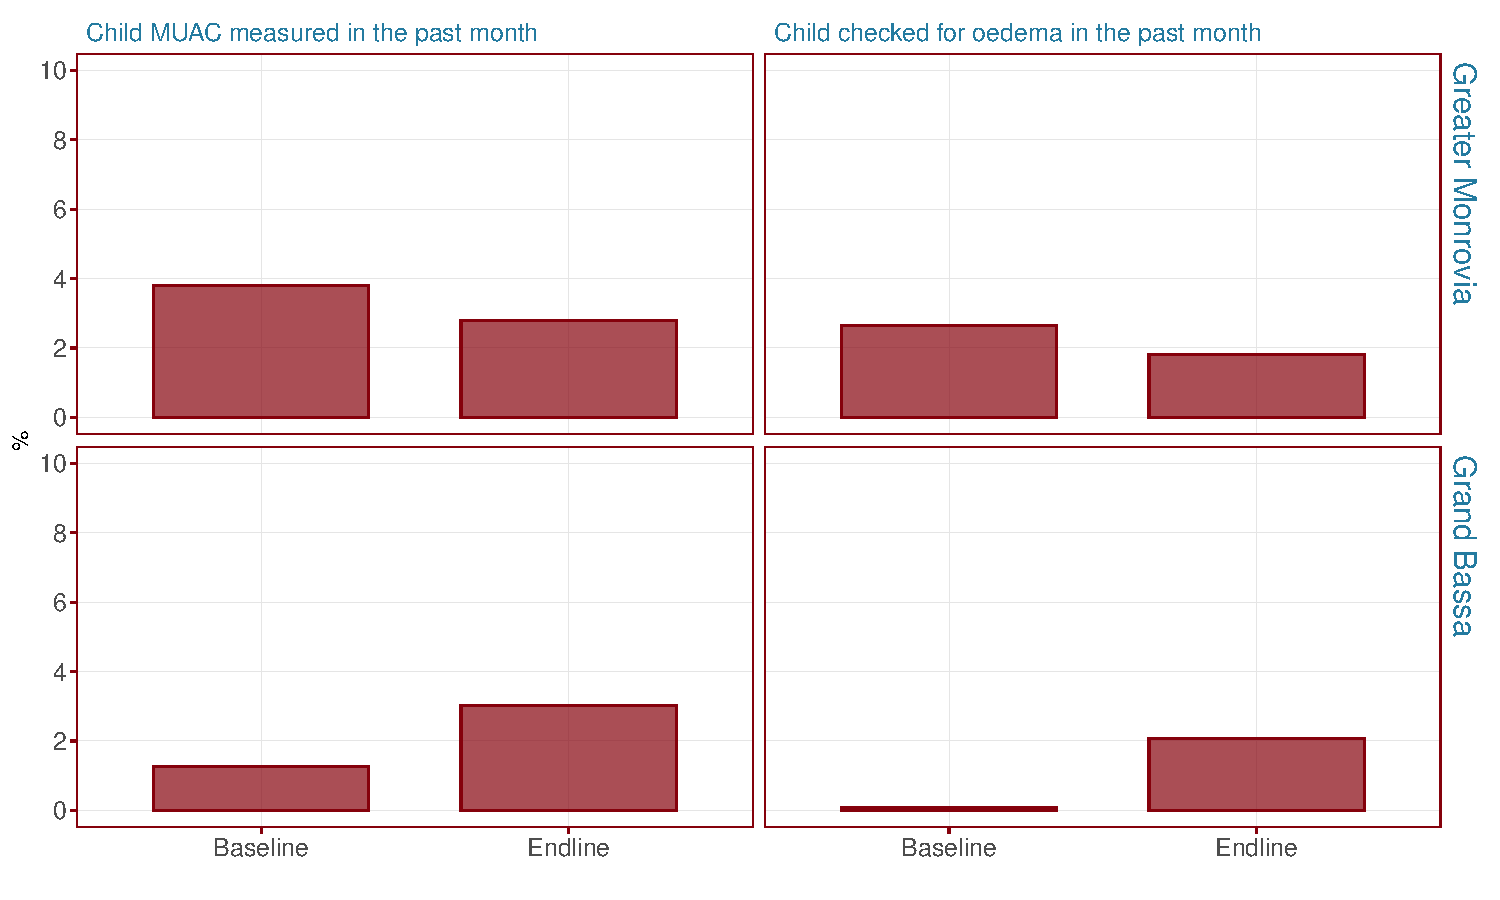
\includegraphics{liberiaCoverageFinalReport_files/figure-latex/screen1-1} 

}

\caption{Acute undernutrition screening coverage}\label{fig:screen1}
\end{figure}

\begin{table}[H]

\caption{\label{tab:screen2}Acute undernutrition screening coverage}
\centering
\fontsize{9}{11}\selectfont
\begin{tabular}[t]{lrrrrrrrrrrrr}
\toprule
\multicolumn{1}{c}{\textbf{ }} & \multicolumn{6}{c}{\textbf{Greater Monrovia}} & \multicolumn{6}{c}{\textbf{Grand Bassa}} \\
\cmidrule(l{3pt}r{3pt}){2-7} \cmidrule(l{3pt}r{3pt}){8-13}
\multicolumn{1}{c}{\textbf{ }} & \multicolumn{3}{c}{\textbf{Baseline}} & \multicolumn{3}{c}{\textbf{Endline}} & \multicolumn{3}{c}{\textbf{Baseline}} & \multicolumn{3}{c}{\textbf{Endline}} \\
\cmidrule(l{3pt}r{3pt}){2-4} \cmidrule(l{3pt}r{3pt}){5-7} \cmidrule(l{3pt}r{3pt}){8-10} \cmidrule(l{3pt}r{3pt}){11-13}
\textbf{Indicator} & \textbf{\makecell[c]{Est\\(\%)}} & \textbf{\makecell[c]{95\%\\LCL}} & \textbf{\makecell[c]{95\%\\UCL}} & \textbf{\makecell[c]{Est\\(\%)}} & \textbf{\makecell[c]{95\%\\LCL}} & \textbf{\makecell[c]{95\%\\UCL}} & \textbf{\makecell[c]{Est\\(\%)}} & \textbf{\makecell[c]{95\%\\LCL}} & \textbf{\makecell[c]{95\%\\UCL}} & \textbf{\makecell[c]{Est\\(\%)}} & \textbf{\makecell[c]{95\%\\LCL}} & \textbf{\makecell[c]{95\%\\UCL}}\\
\midrule
\rowcolor{gray!6}  Child MUAC measured in the past month & 3.79 & 1.37 & 7.73 & 2.8 & 1.90 & 3.83 & 1.26 & 0.81 & 1.92 & 3.03 & 1.34 & 5.45\\
Child checked for oedema in the past month & 2.65 & 0.52 & 6.63 & 1.8 & 1.07 & 2.54 & 0.07 & 0.00 & 0.21 & 2.08 & 0.89 & 4.10\\
\bottomrule
\end{tabular}
\end{table}

\begin{figure}[H]

{\centering 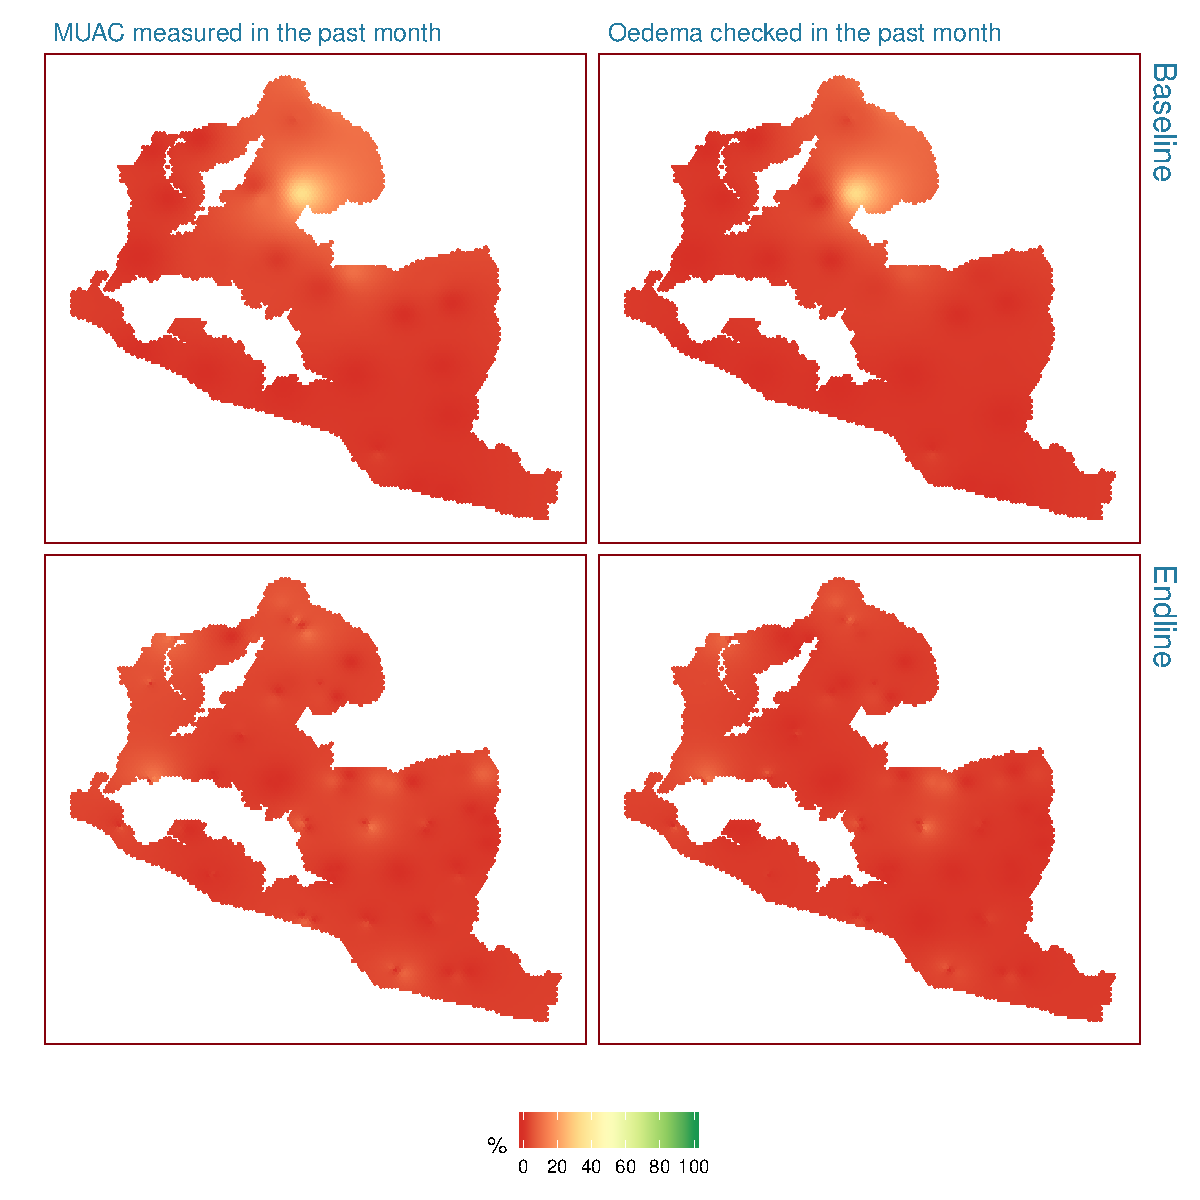
\includegraphics{liberiaCoverageFinalReport_files/figure-latex/screen1map-1} 

}

\caption{Spatial distribution of acute undernutrition screening coverage in Greater Monrovia}\label{fig:screen1map}
\end{figure}

\begin{figure}[H]

{\centering 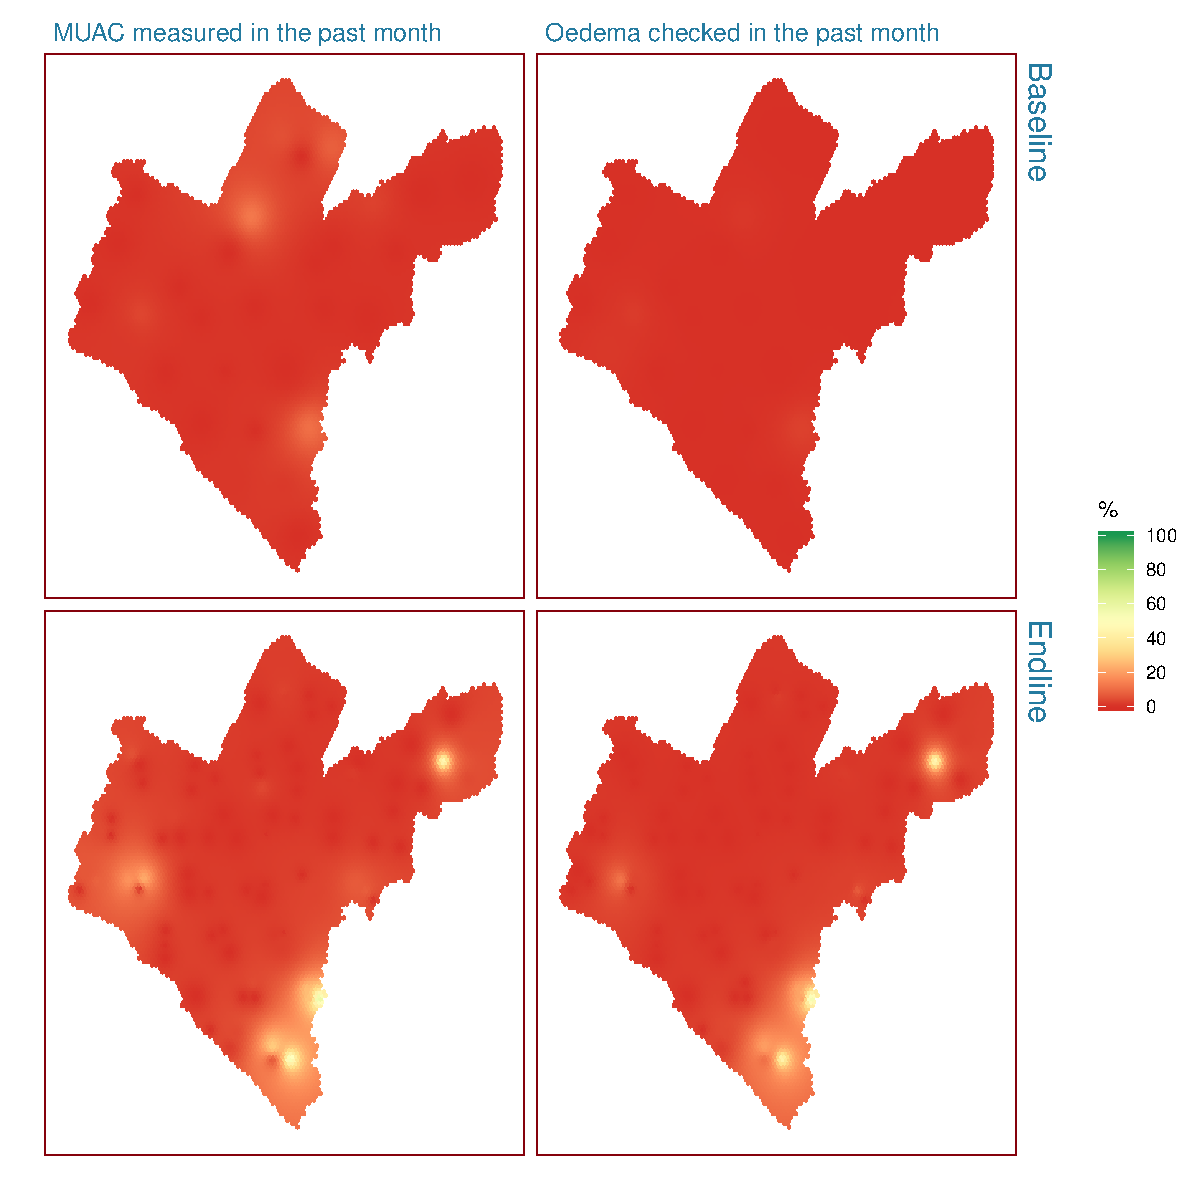
\includegraphics{liberiaCoverageFinalReport_files/figure-latex/screen2map-1} 

}

\caption{Spatial distribution of acute undernutrition screening coverage in Grand Bassa}\label{fig:screen2map}
\end{figure}

\newpage

\hypertarget{cmam-coverage-1}{%
\subsection{CMAM Coverage}\label{cmam-coverage-1}}

Case-finding effectiveness in both Greater Monrovia and Grand Bassa are low at baseline (see Figure \ref{fig:cmam1plot} and Table \ref{tab:cmam1table}) with Greater Monrovia having a higher rate at about 31\% compared to 6\% in Grand Bassa. At endline, Greater Monrovia's case-finding effectiveness dropped significantly to just about 15\% while Grand Bassa's case-finding effectiveness stayed about the same.

Treatment coverage is at 55\% in Greater Monrovia at baseline which is an improvement from previous coverage estimates for the area but Grand Bassa only managed to get 18\% treatment coverage. At endline, treatment coverage in Greater Monrovia dropped to less than 30\% while treatment coverage in Grand Bassa decreased slightly to about 13\%. The drop in coverage of CMAM for Greater Monrovia is statistically signficant.

\begin{figure}[H]

{\centering 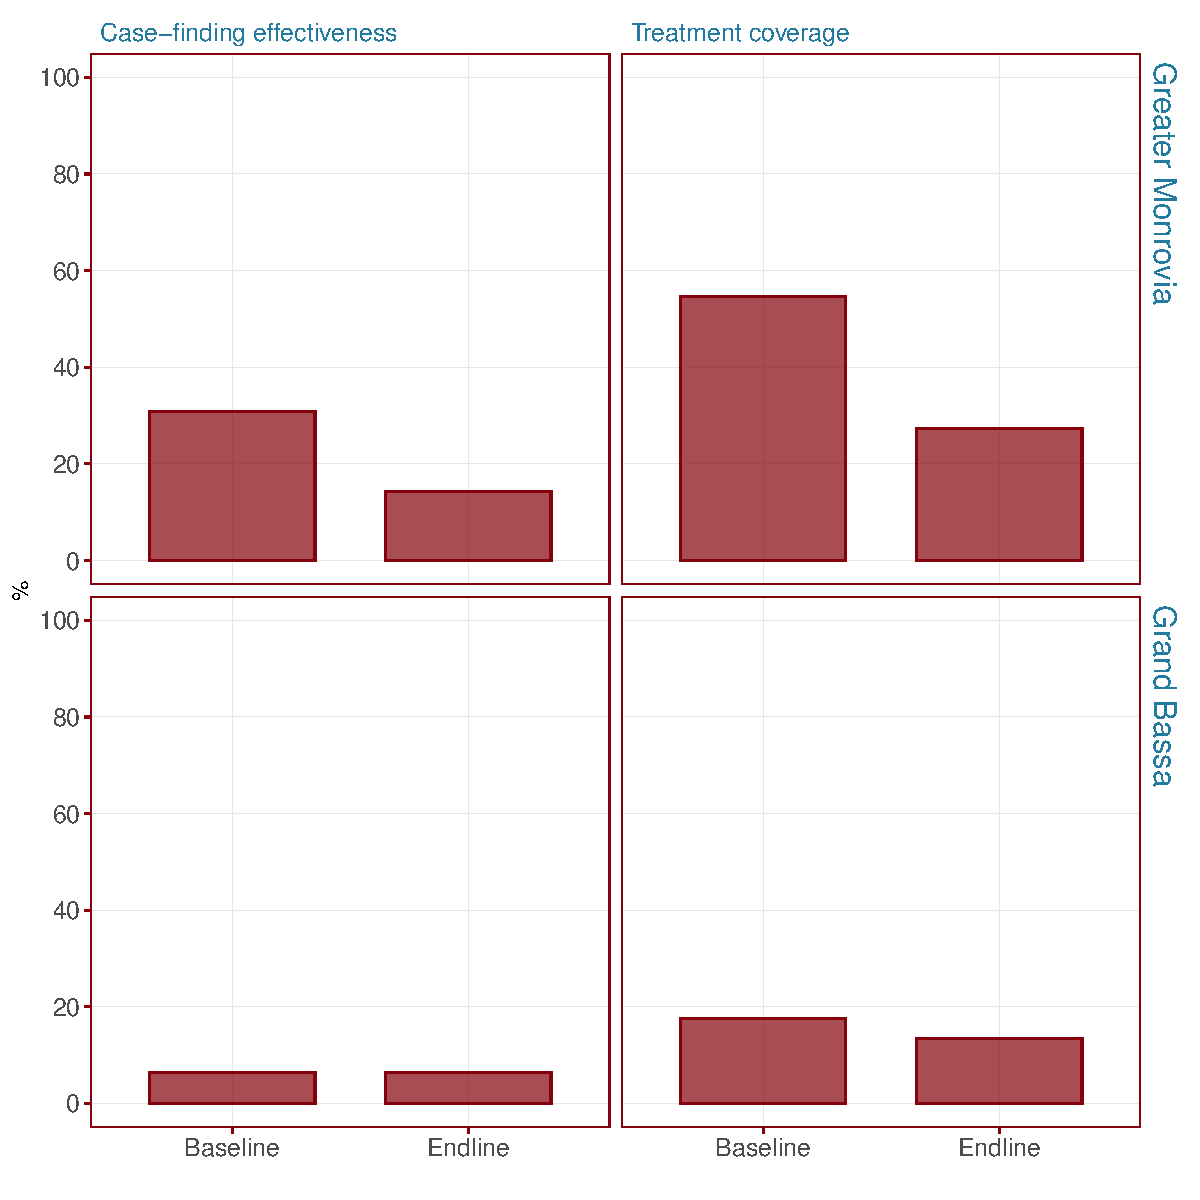
\includegraphics{liberiaCoverageFinalReport_files/figure-latex/cmam1plot-1} 

}

\caption{CMAM coverage}\label{fig:cmam1plot}
\end{figure}

\begin{table}[H]

\caption{\label{tab:cmam1table}CMAM coverage}
\centering
\fontsize{9}{11}\selectfont
\begin{tabular}[t]{lrrrrrrrrrrrr}
\toprule
\multicolumn{1}{c}{\textbf{ }} & \multicolumn{6}{c}{\textbf{Monrovia}} & \multicolumn{6}{c}{\textbf{Grand Bassa}} \\
\cmidrule(l{3pt}r{3pt}){2-7} \cmidrule(l{3pt}r{3pt}){8-13}
\multicolumn{1}{c}{\textbf{ }} & \multicolumn{3}{c}{\textbf{Baseline}} & \multicolumn{3}{c}{\textbf{Endline}} & \multicolumn{3}{c}{\textbf{Baseline}} & \multicolumn{3}{c}{\textbf{Endline}} \\
\cmidrule(l{3pt}r{3pt}){2-4} \cmidrule(l{3pt}r{3pt}){5-7} \cmidrule(l{3pt}r{3pt}){8-10} \cmidrule(l{3pt}r{3pt}){11-13}
\textbf{Indicator} & \textbf{\makecell[c]{Est\\(\%)}} & \textbf{\makecell[c]{95\%\\LCL}} & \textbf{\makecell[c]{95\%\\UCL}} & \textbf{\makecell[c]{Est\\(\%)}} & \textbf{\makecell[c]{95\%\\LCL}} & \textbf{\makecell[c]{95\%\\UCL}} & \textbf{\makecell[c]{Est\\(\%)}} & \textbf{\makecell[c]{95\%\\LCL}} & \textbf{\makecell[c]{95\%\\UCL}} & \textbf{\makecell[c]{Est\\(\%)}} & \textbf{\makecell[c]{95\%\\LCL}} & \textbf{\makecell[c]{95\%\\UCL}}\\
\midrule
\rowcolor{gray!6}  Case-finding effectiveness & 30.77 & 27.29 & 34.25 & 14.29 & 12.89 & 15.69 & 6.45 & 4.90 & 8.00 & 6.38 & 5.36 & 7.40\\
Treatment coverage & 54.68 & 53.97 & 55.38 & 27.35 & 26.60 & 28.10 & 17.65 & 16.77 & 18.53 & 13.48 & 12.73 & 14.24\\
\bottomrule
\end{tabular}
\end{table}

The spatial distribution of CMAM coverage in Greater Monrovia is shown in Figure \ref{fig:cmamMap1}. It shows high levels of coverage at baseline throughout most of Greater Monrovia but with significant areas of low coverage in the western and southeastern sections. At endline, case-finding effectiveness and treatment coverage is low throughout the whole of Greater Monrovia with very little spatial variation.

The spatial distribution of CMAM coverage in Grand Bassa is shown in Figure \ref{fig:cmamMap2}. Coverage at baseline in Grand Bassa is low throughout but with pockets of high coverage in the western area of the county. At endline, the case-finding effectiveness and treatment coverage of CMAM in Grand Bassa is still generally low but with lighter hotspots than baseline. Areas of high coverage in the west of the county has increased.

\begin{figure}[H]

{\centering 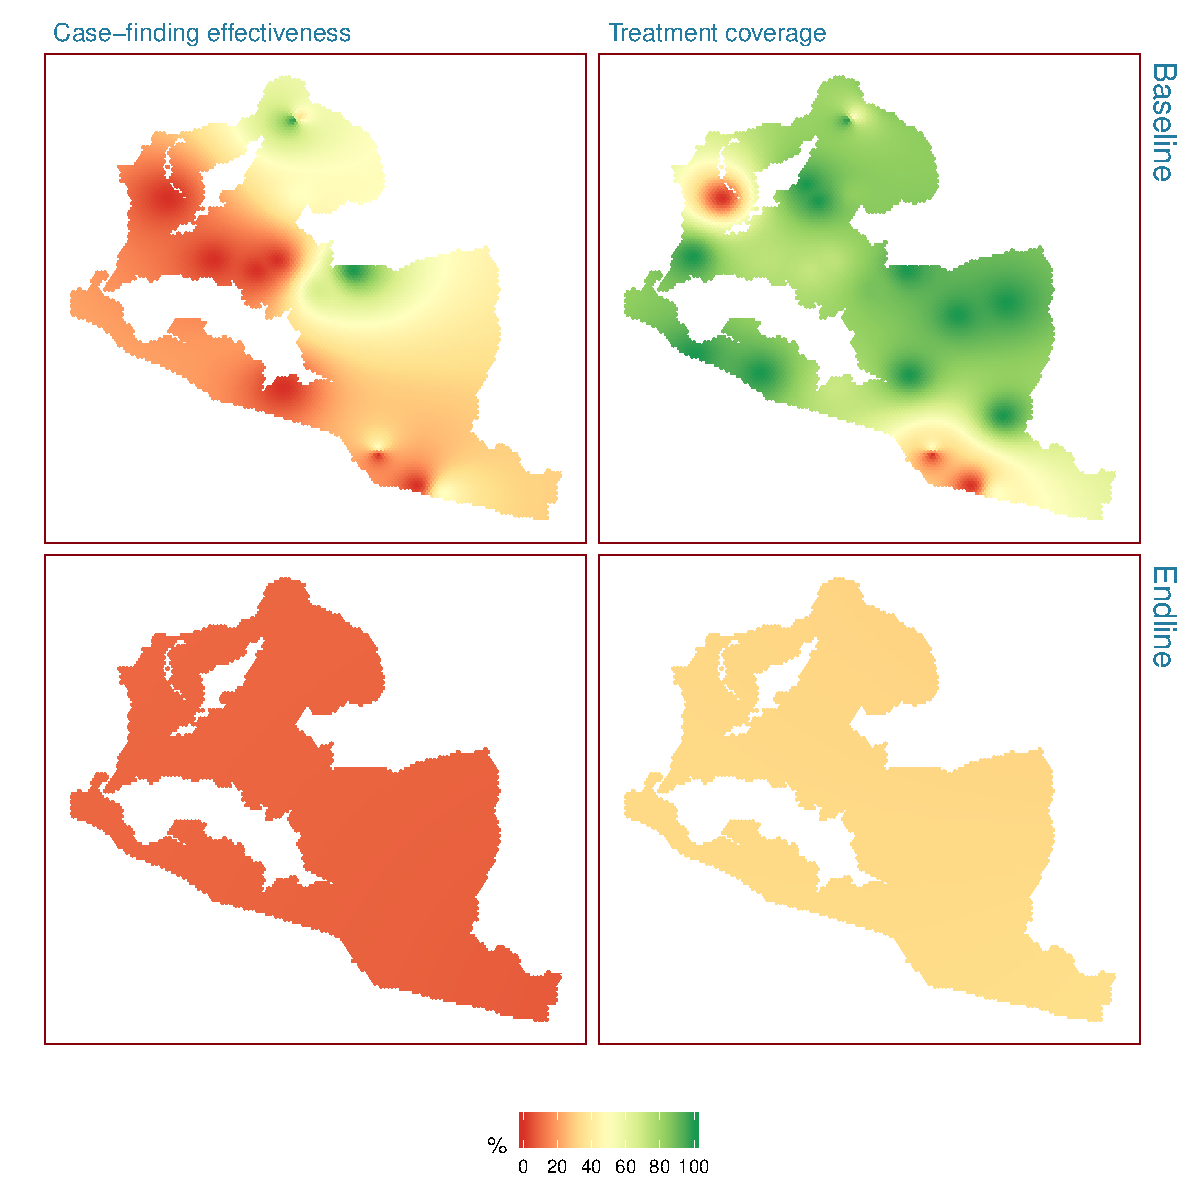
\includegraphics{liberiaCoverageFinalReport_files/figure-latex/cmamMap1-1} 

}

\caption{Spatial distribution of CMAM coverage in Greater Monrovia}\label{fig:cmamMap1}
\end{figure}

\begin{figure}[H]

{\centering 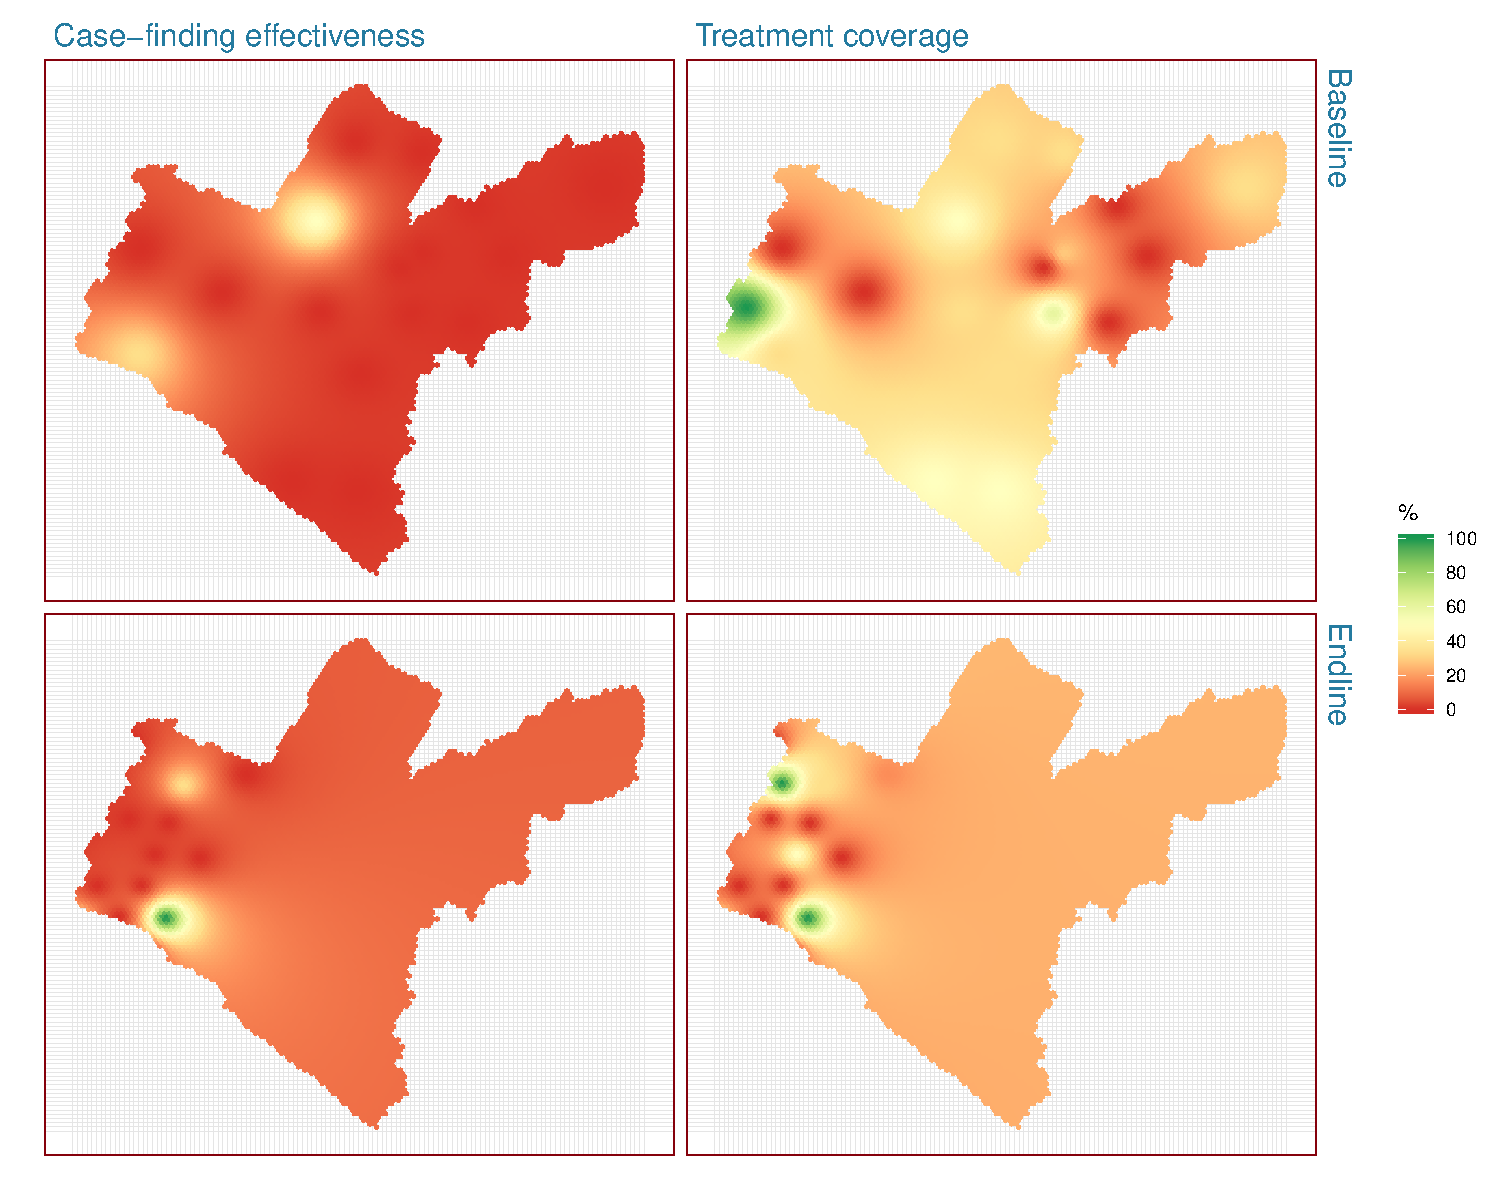
\includegraphics{liberiaCoverageFinalReport_files/figure-latex/cmamMap2-1} 

}

\caption{Spatial distribution of CMAM coverage in Grand Bassa}\label{fig:cmamMap2}
\end{figure}

For SAM cases not covered by the programme, Figure \ref{fig:cmam2plot} summarises the reasons for non-coverage. No knowledge of the treatment modality for acute undernutrition was consistently the reason reported by non-covered cases at baseline and endline in both areas.

\begin{figure}[H]

{\centering 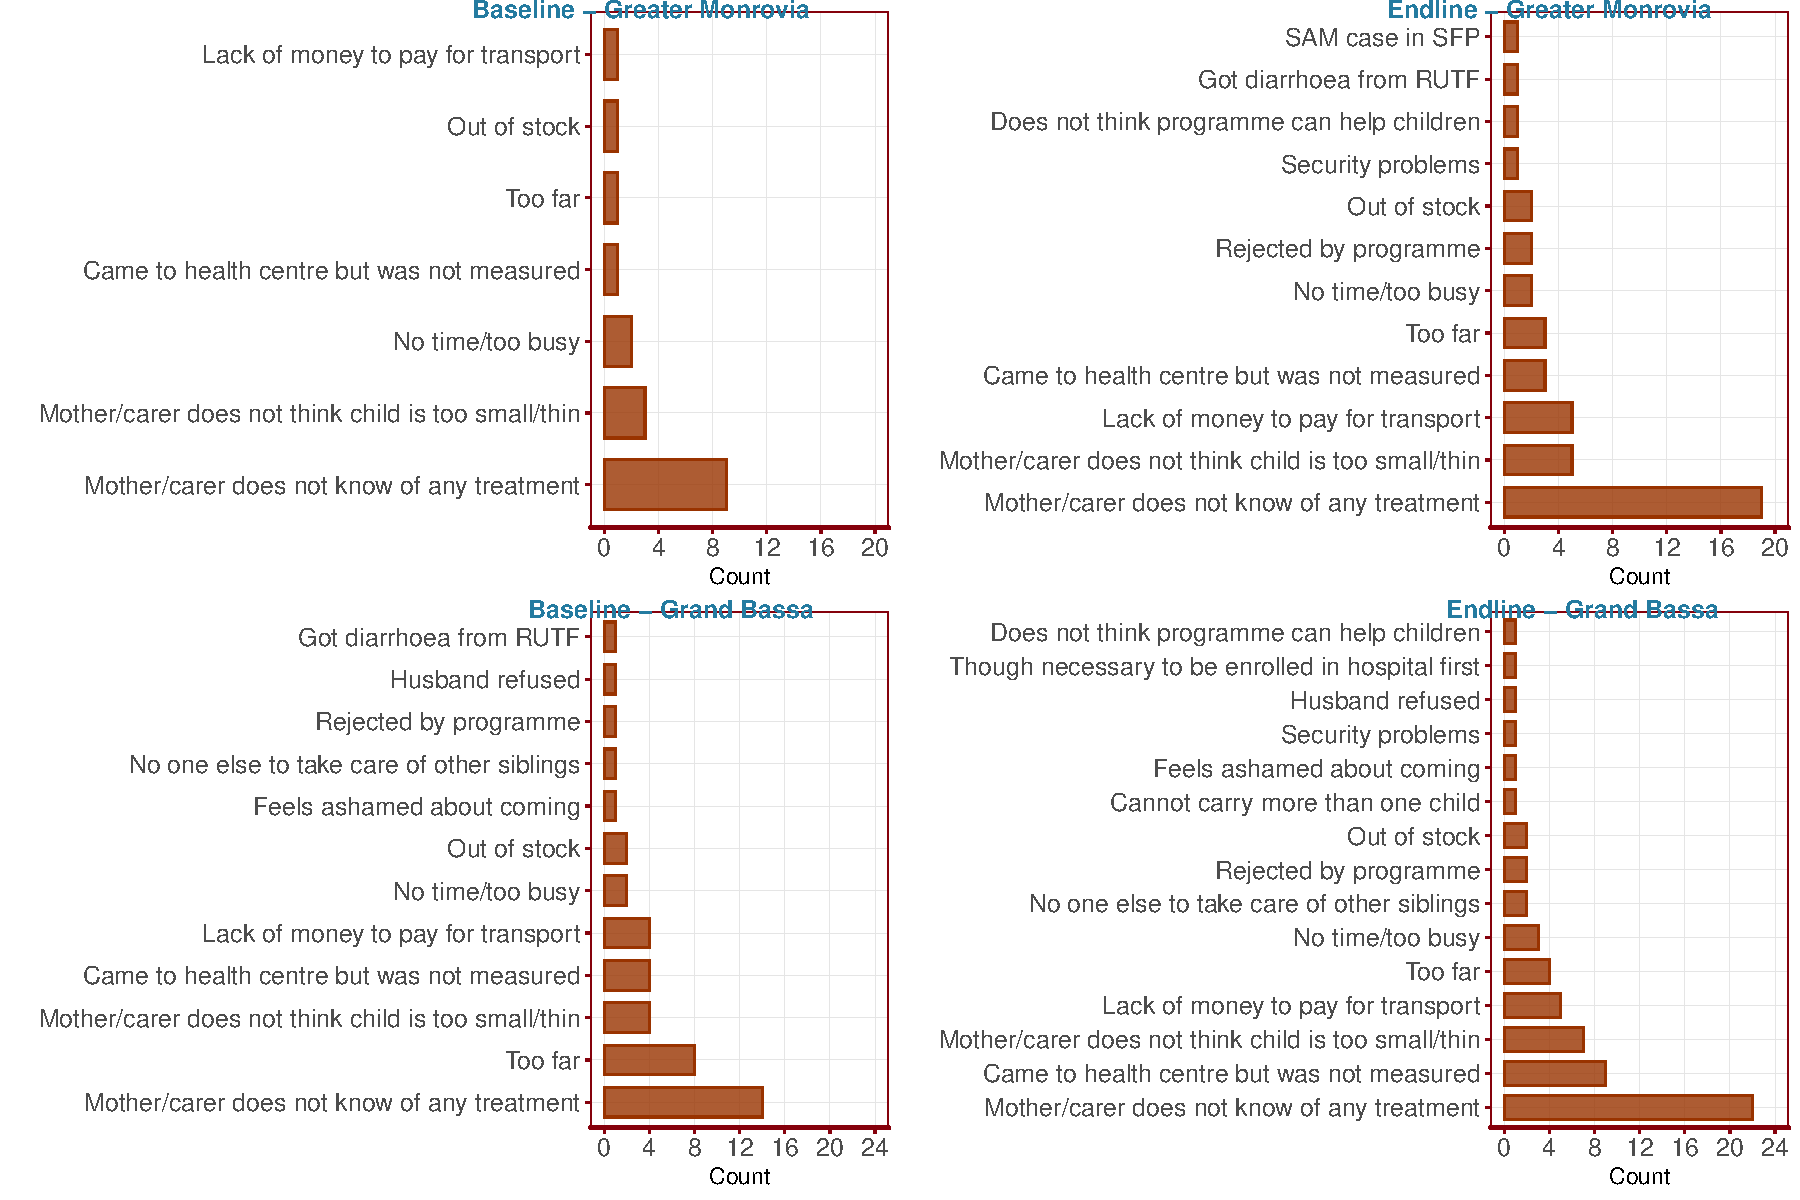
\includegraphics{liberiaCoverageFinalReport_files/figure-latex/cmam2plot-1} 

}

\caption{Reasons for not being in CMAM programme}\label{fig:cmam2plot}
\end{figure}

\hypertarget{discussion}{%
\section{Discussion}\label{discussion}}

The results of the coverage assessment of direct nutrition interventions in Liberia specifically in Greater Monrovia and Grand Bassa indicate various levels of disparity in coverage both between the programme areas and within the programme areas assessed.

Long-standing programmes such as IFA supplementation, IYCF counselling and vitamin A supplementation have performed fairly well in terms of coverage. The majority of women and children targeted by these programmes are knowledgeable of the programme and are beneficiaries of the programme. Years of implementation complemented by the level of support and investment by the government and its partners seem to have paid dividends in allowing for these programmes to reach almost all of their targeted beneficiaries. However, there is still much room for improvement and the current coverage levels can still be improved and increased.

For IFA supplementation, the programme has been able to reach most mothers and has been successful in getting them to take IFA supplements. However, the key challenge for the programme now is to keep mothers taking the tablets for the recommended period of time (at least 90 days). Since the survey did not collect data on mother's reasons for stopping IFA tablet consumption, it would be a good first step for the factors for stopping IFA tablet consumption be investigated with the results used as the basis for further counselling and education provided for pregnant women. Given that contact with health care services during pregnancy is high, it would be good to review existing guidance provided through ANC regarding the intake of IFA and to see whether relevant and appropriate information that addresses pregnant women's reasons for stopping are clarified and addressed.

For IYCF counselling, coverage of the counselling activities is high. It would now be important to assess the next level in the coverage hierarchy of whether mothers practice what they have been taught or what they have learned. The most straightforward way of doing so would be assessing IYCF practices as these are the key behaviours that are targeted by the counselling. If this was to be considered, however, UNICEF and its partners would have to take into account the fact that current standard IYCF indicators can only be assessed through big sample surveys such as DHS and MICS. Yet these surveys would most likely not provide the same level of detail and information as the current assessment. There are, however, small sample alternatives to the standard IYCF indicators such as the Infant and Child Feeding Index (ICFI) indicator set which can be considered for use in routine monitoring of IYCF practices \citep{Guevarra:2016uw}.

For vitamin A supplementation, the current figures are relatively lower than the expected indirect coverage estimates produced by government. It would be important to see what the potential reasons for this disparity are and to ensure that vaccination campaigns, to which vitamin A supplementation is generally attached, ensures the availability of vitamin A and optimises the synergies between vitamin A supplementation and vaccination given that it seems availability of vitamin A and access to vaccination is a factor for non-coverage to vitamin A.

Programmes such as MNP and CMAM, on the other hand, show how new and recently scaled-up programmes are still in the process of achieving the highest levels of coverage possible. MNP supplementation which is the newest programme of those assessed is understandably still struggling with coverage even at endline. Knowledge of the programme and knowlege of how the programme works and its importance for children's health and nutrition is the key falter point which is typical of a programme at this stage of its evolution. The programme is mainly anchored to the health centre and therefore knowledge and access to it is primarily influenced by mothers' behaviours and attitudes towards seeking care and treatment at the health facility. Given that MNP is aimed at children who are otherwise healthy (not acute malnourished), the current MNP coverage estimates indicate that health-seeking behaviour leading to a visit to a health facility is mainly influenced by whether their children are sick rather than as a way to seek information or participate in promotive and preventive services such as MNP supplementation. Other factors include physical access to health centres. A more community-based approach to MNP supplementation that is integrated with other community-based programmes such as vaccinations and CMAM should be considered as a potential delivery mechanism. Screening of children using MUAC can be integrated into vaccination campaigns and children under 2 years old identified as not being acutely malnourished are informed about MNP supplementation programme and ideally provided with the MNP supplements at point of contact.

Finally, for CMAM which is not entirely new but still in its early stages of scale-up, the coverage estimates at baseline and endline indicate 1) disparity between Greater Monrovia and Grand Bassa in terms of the level and intensity of the community aspects of the programme; 2) signficant drop in coverage of CMAM in Greater Monrovia given that at baseline its coverage was exemplary for an urban CMAM programme; and, 3) no significant change in coverage of CMAM in Grand Bassa with coverage still remaining unacceptably low. At baseline, screening and case-finding in Greater Monrovia is better than in Grand Bassa and this can partly explain the difference in treatment coverage between the two areas at baseline. At endline, no improvement in screening has happened and the levels of coverage for CMAM has signficantly plummetted. Based on feedback by stakeholders, this has been attributed to government being the main service provider for CMAM in the past year as usual stakeholders that supported government were not engaged due to several programmatic issues. This points to the need for ensuring increased and continued capacity building of government in CMAM and other related interventions so that they can be truly in a position that they can implement and maintain these programmes with or without external support.

Lessons learned from the years of implementation of the IFA and vitamin A programmes can be useful in improving coverage of MNP and CMAM particularly with potential integration of these services into a unified and coherent child health and nutrition programme in Liberia.

\newpage

\hypertarget{annex-a-survey-instruments}{%
\section*{Annex A: Survey instruments}\label{annex-a-survey-instruments}}
\addcontentsline{toc}{section}{Annex A: Survey instruments}

The following tabular form was used for the CMAM coverage assessment:

\begin{center}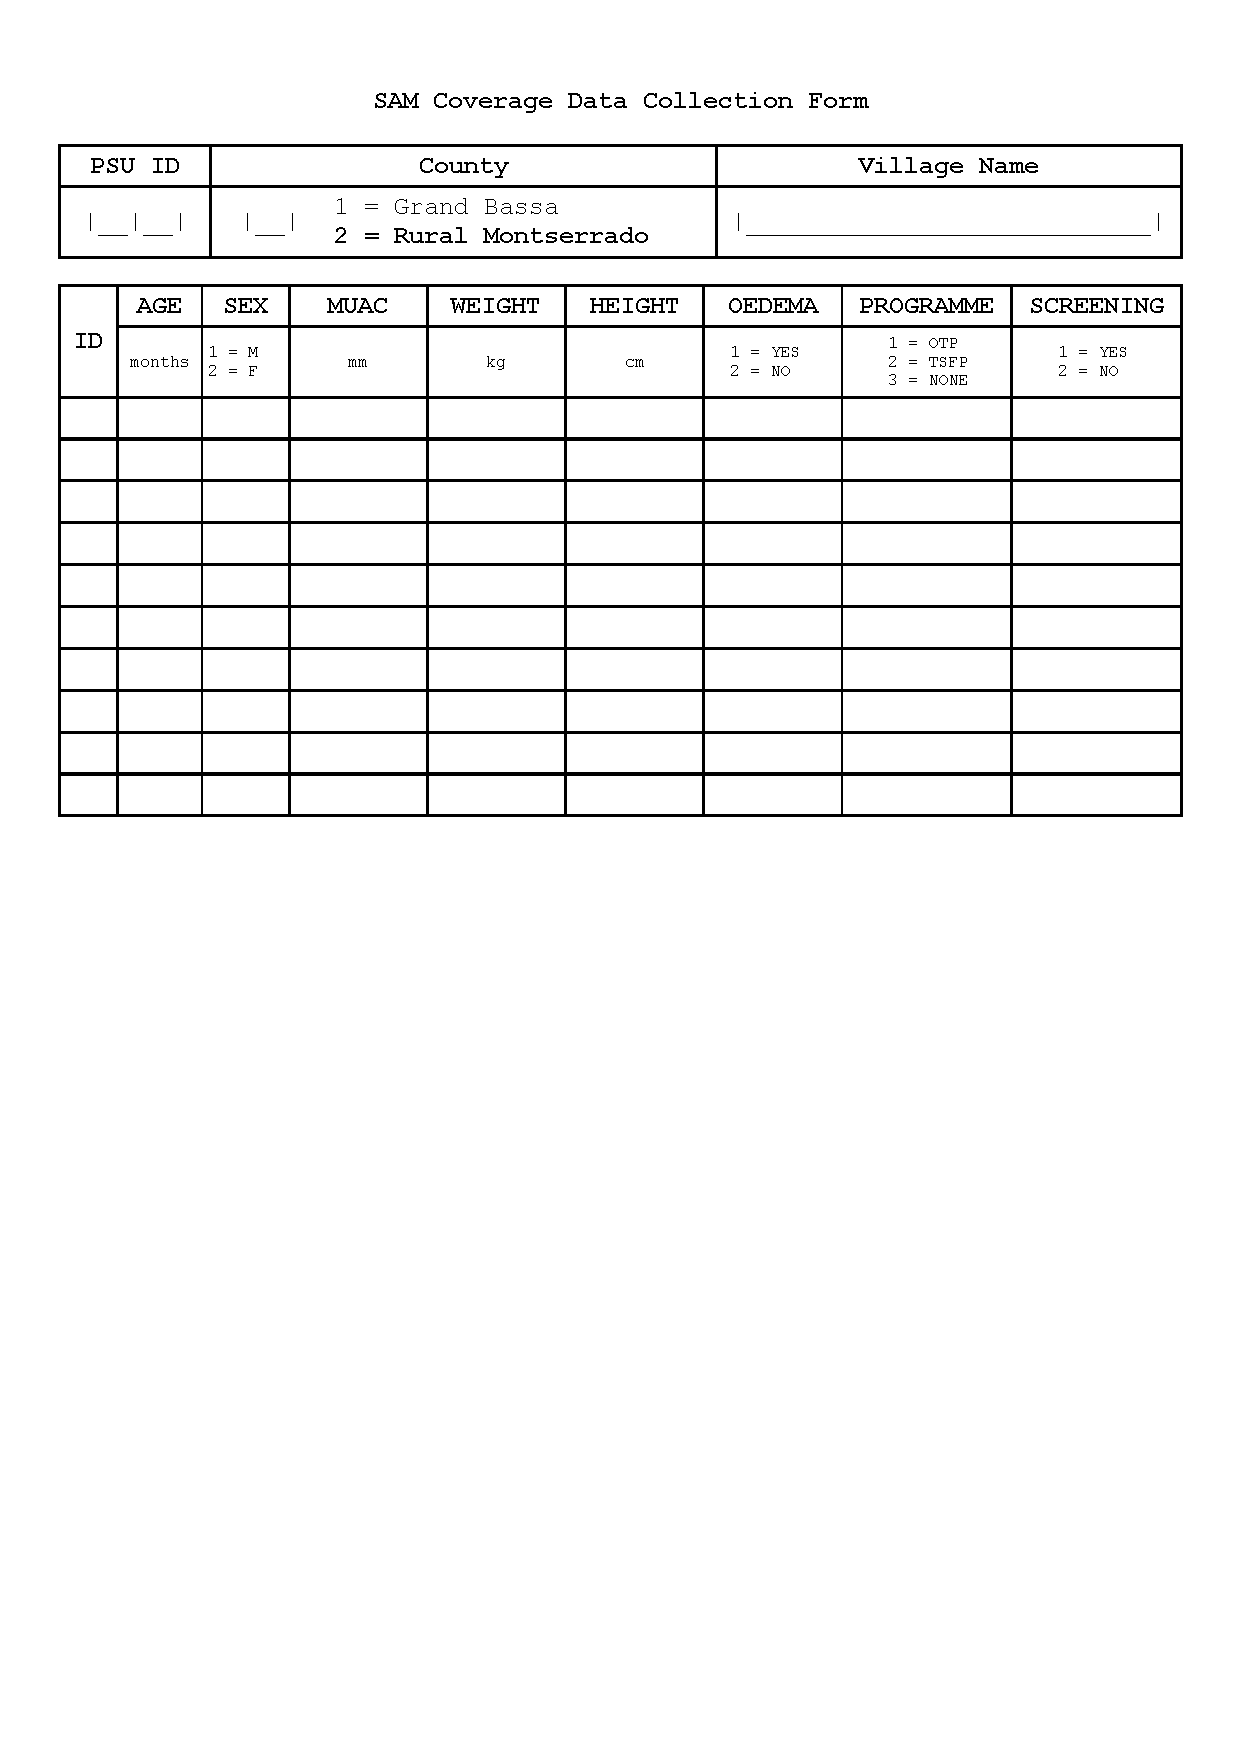
\includegraphics[width=0.9\linewidth]{forms/samForm} \end{center}

The data collected using the tabular forms allows for estimation of coverage. They do not, however, allow one to know the reasons for coverage failure. To collect this data we applied a ``barriers'' questionnaire to the mothers/carers of uncovered SAM cases. Here is an example of a barriers questionnaire:

\newpage

\begin{center}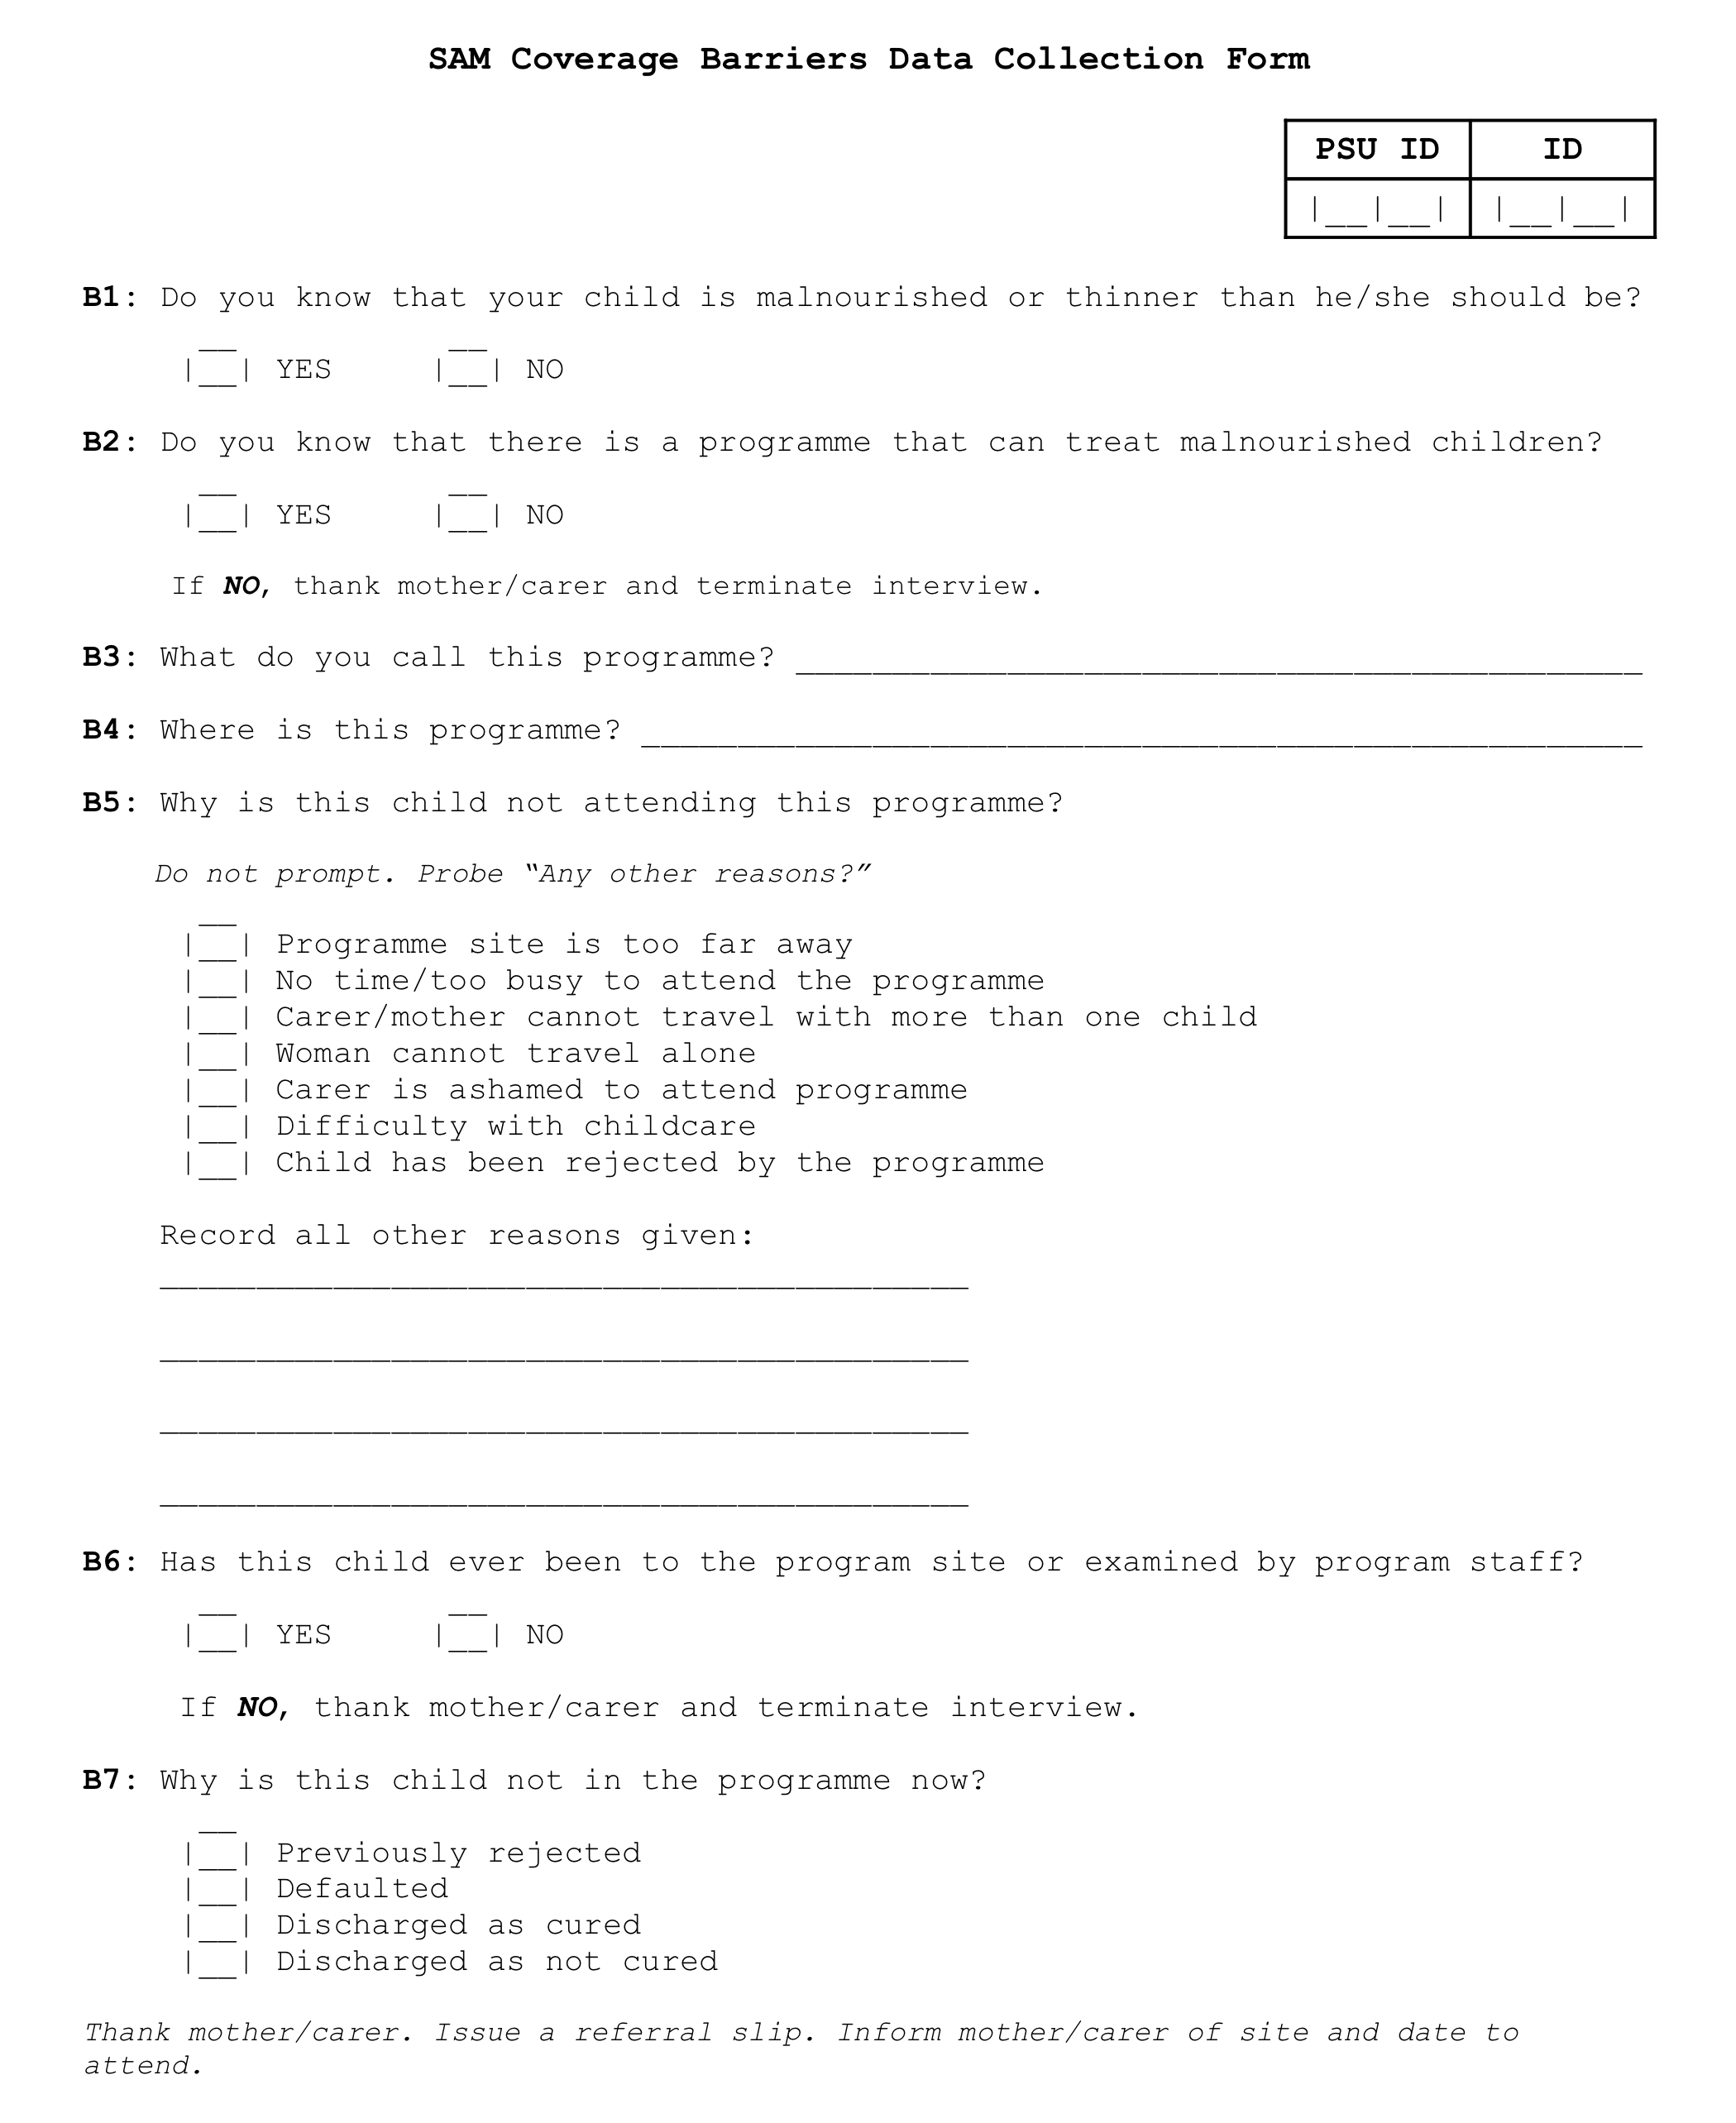
\includegraphics[width=0.9\linewidth]{forms/samBarriersForm} \end{center}

\textbf{CMAM coverage survey instruments}

The CMAM coverage surveys primarily used two forms. The first form was used to collect coverage data from SAM children found during the survey. Given that this survey used house-to-house/door-to-door sampling for stage 2, then it was necessary to record all data from all children that were measured with MUAC and oedema.

\textbf{Survey for children 6-59 months and their mothers}

For the survey for children 6-59 months, following is a sample/template questionnaire used.

\begin{center}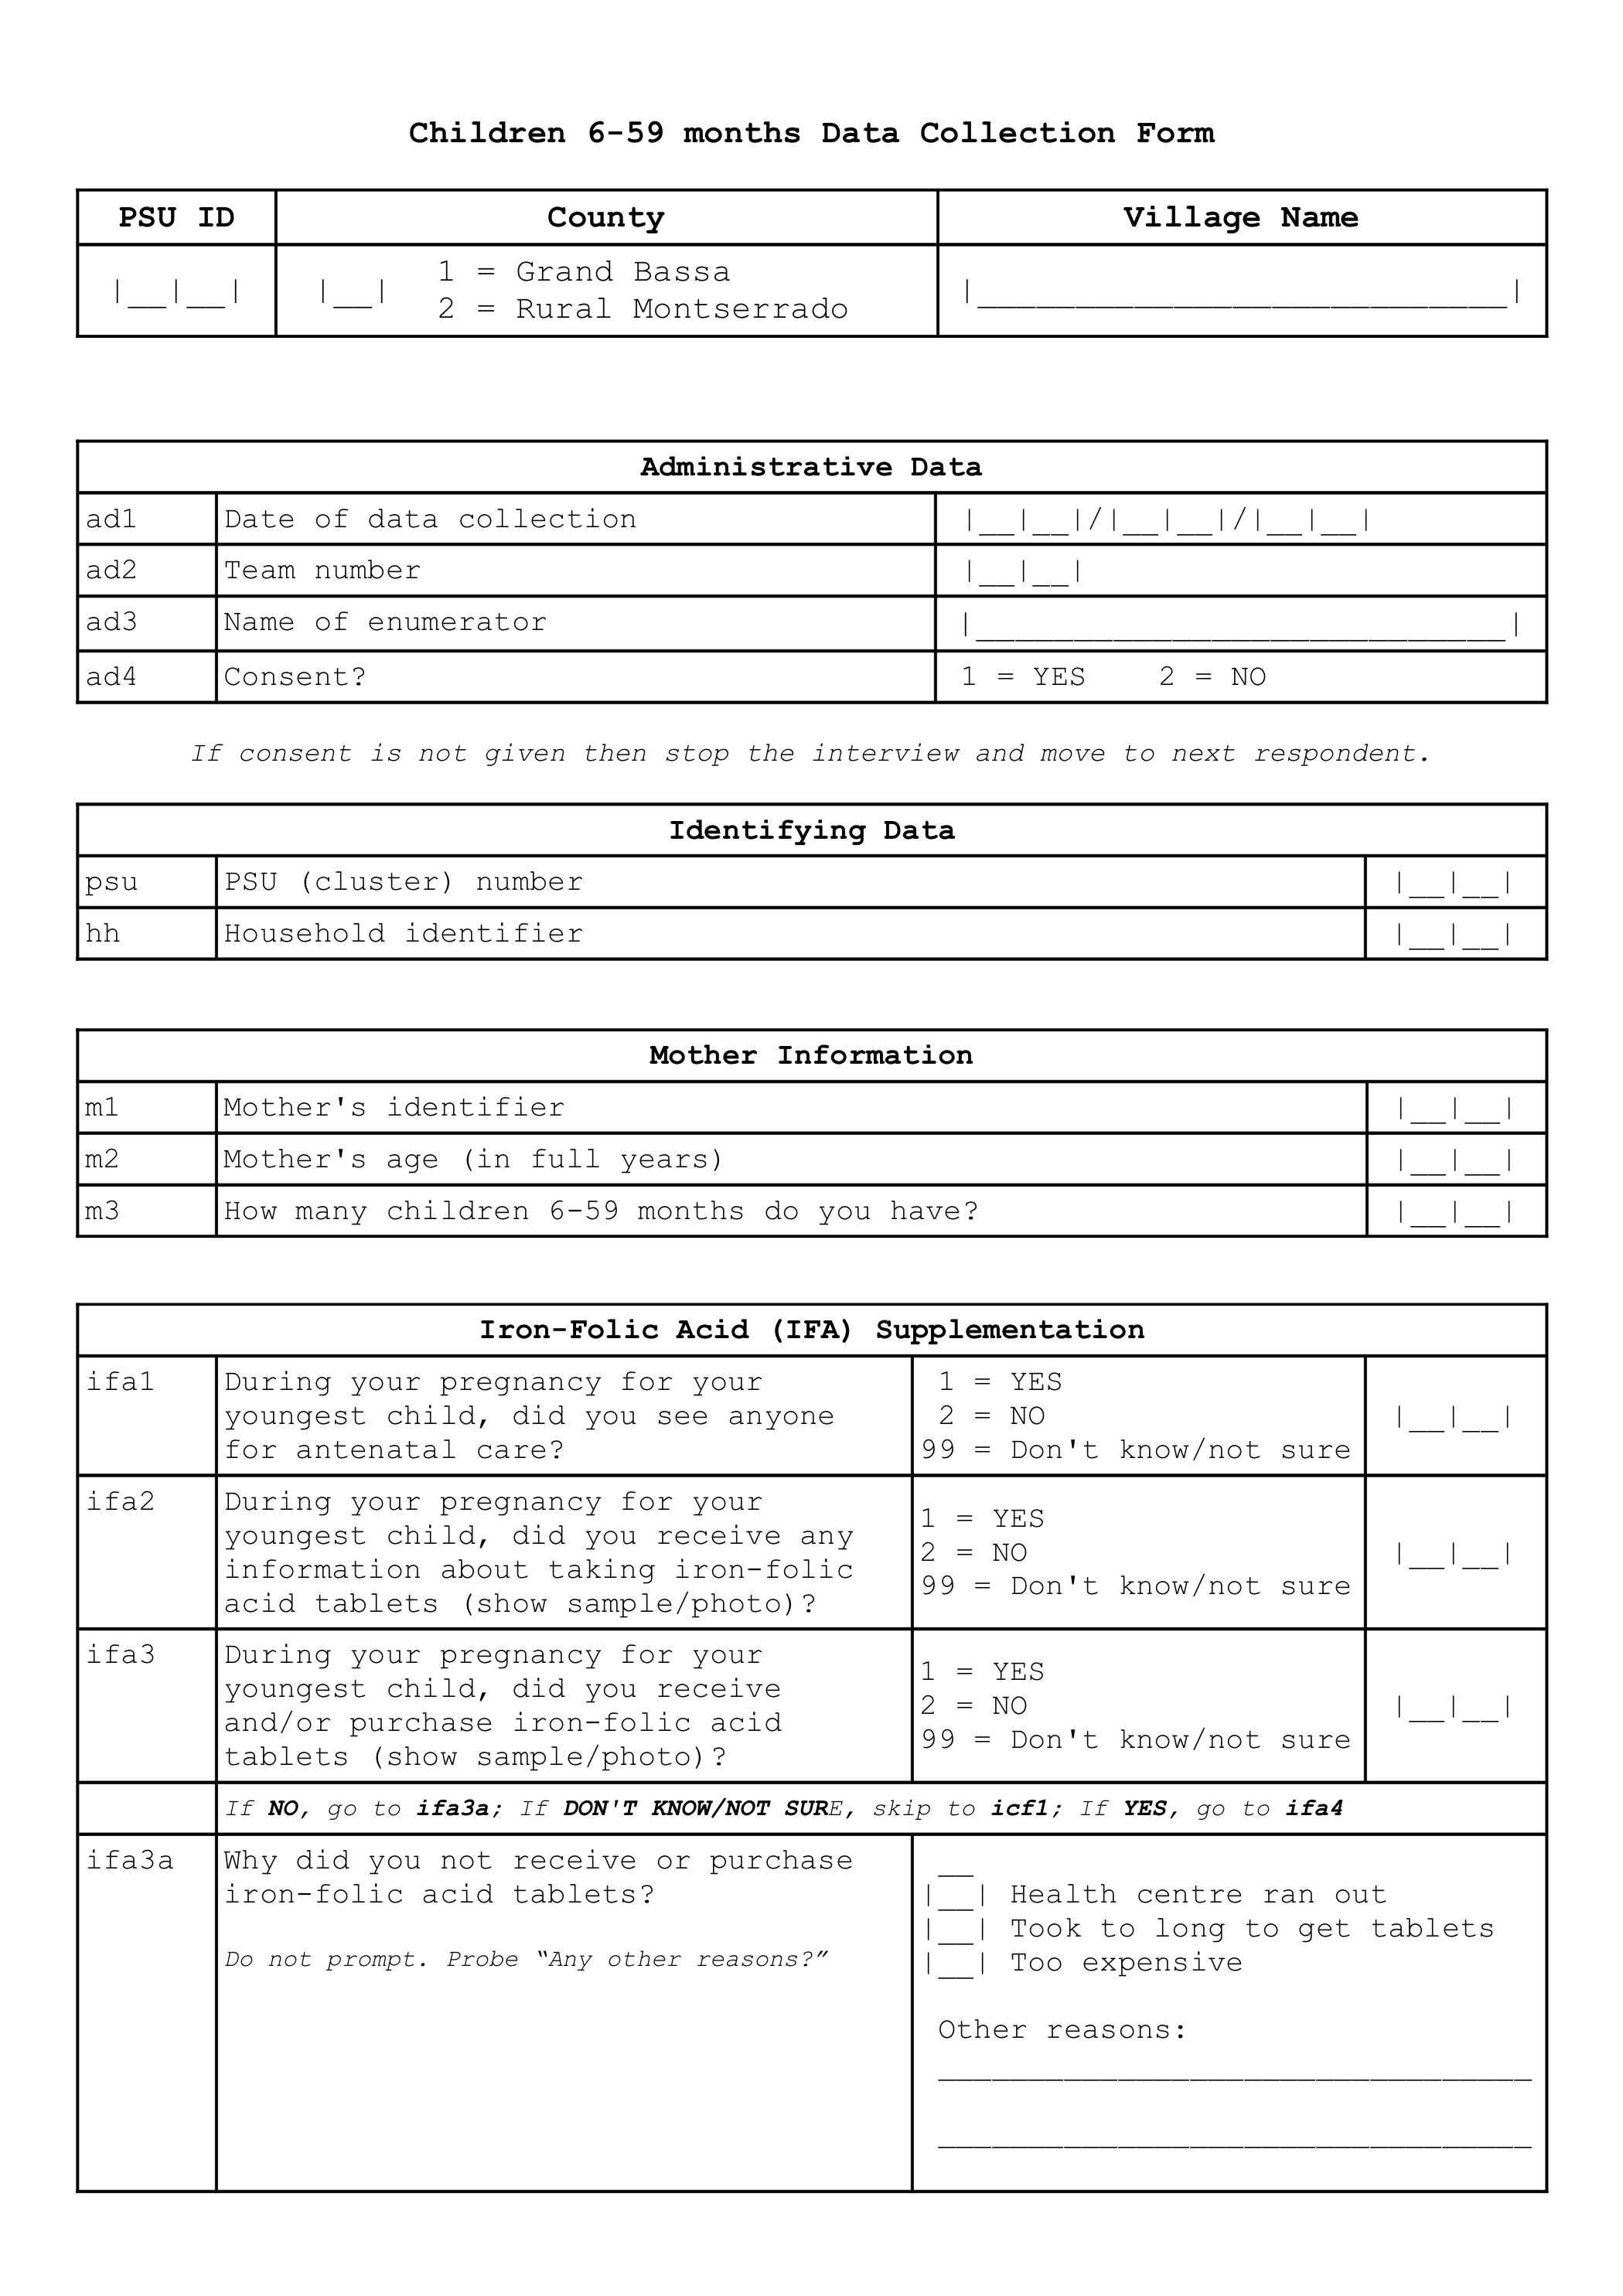
\includegraphics[width=0.9\linewidth]{forms/childForm1} \end{center}

\begin{center}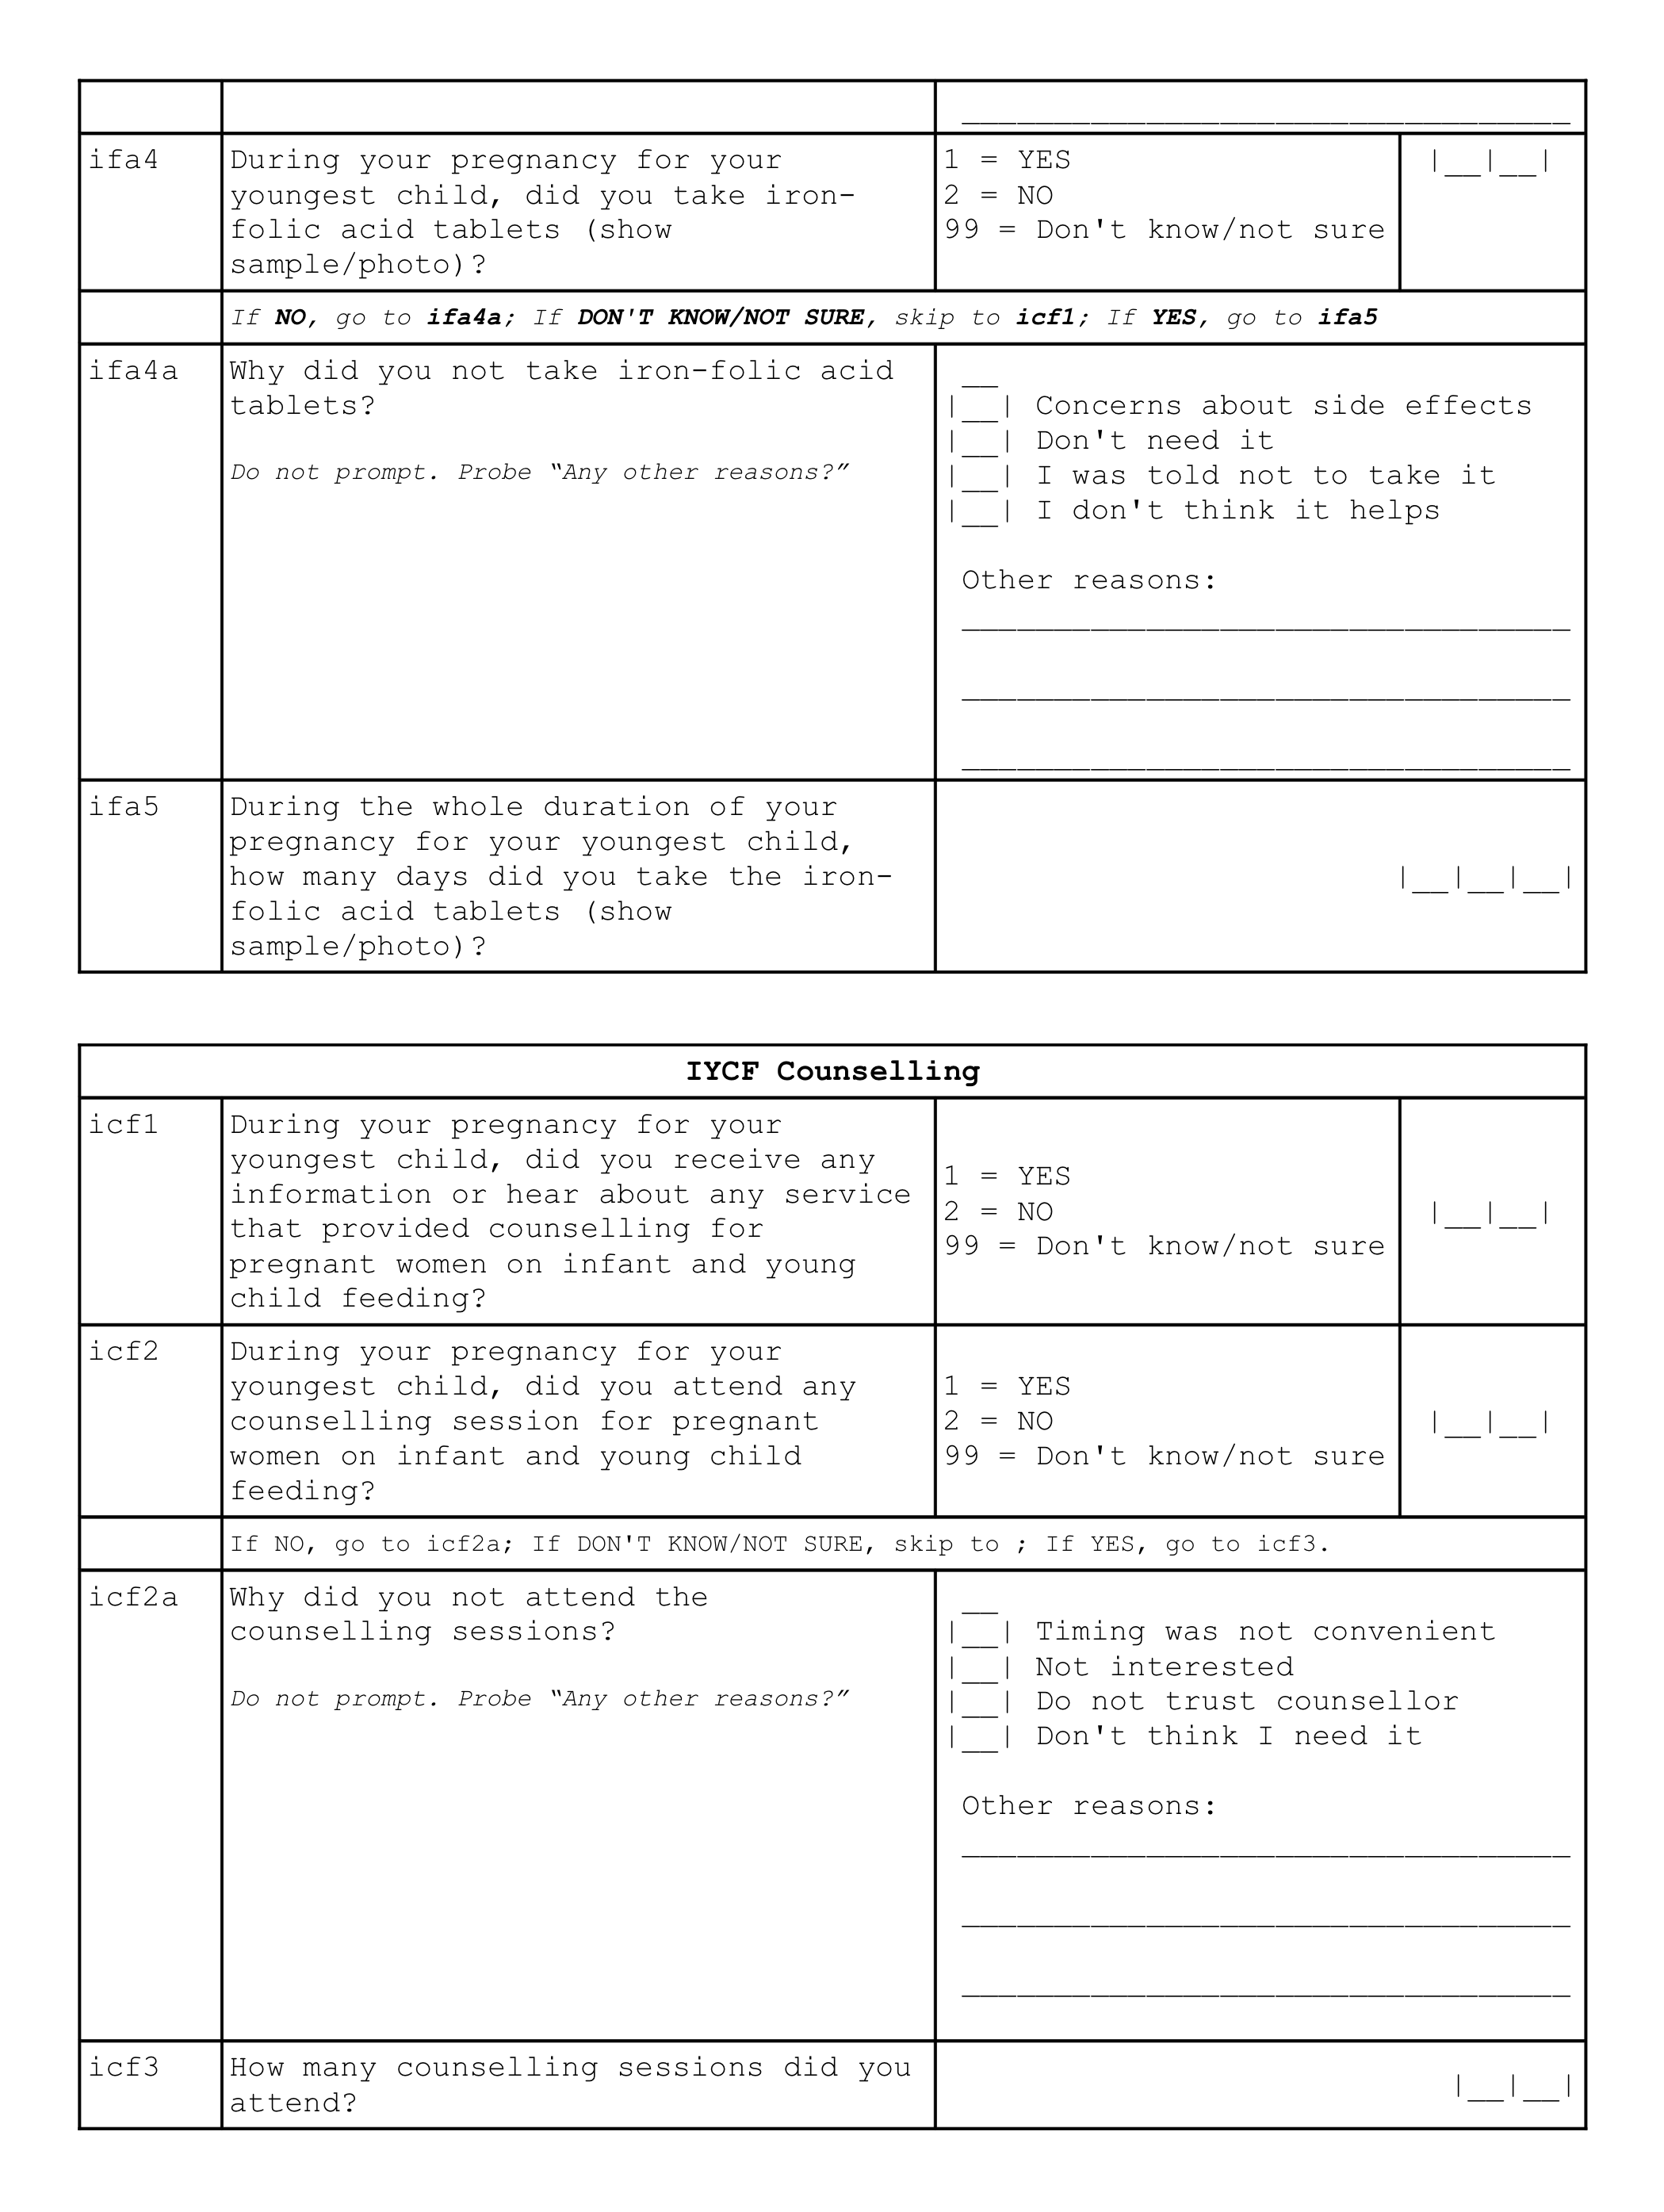
\includegraphics[width=0.9\linewidth]{forms/childForm2} \end{center}

\begin{center}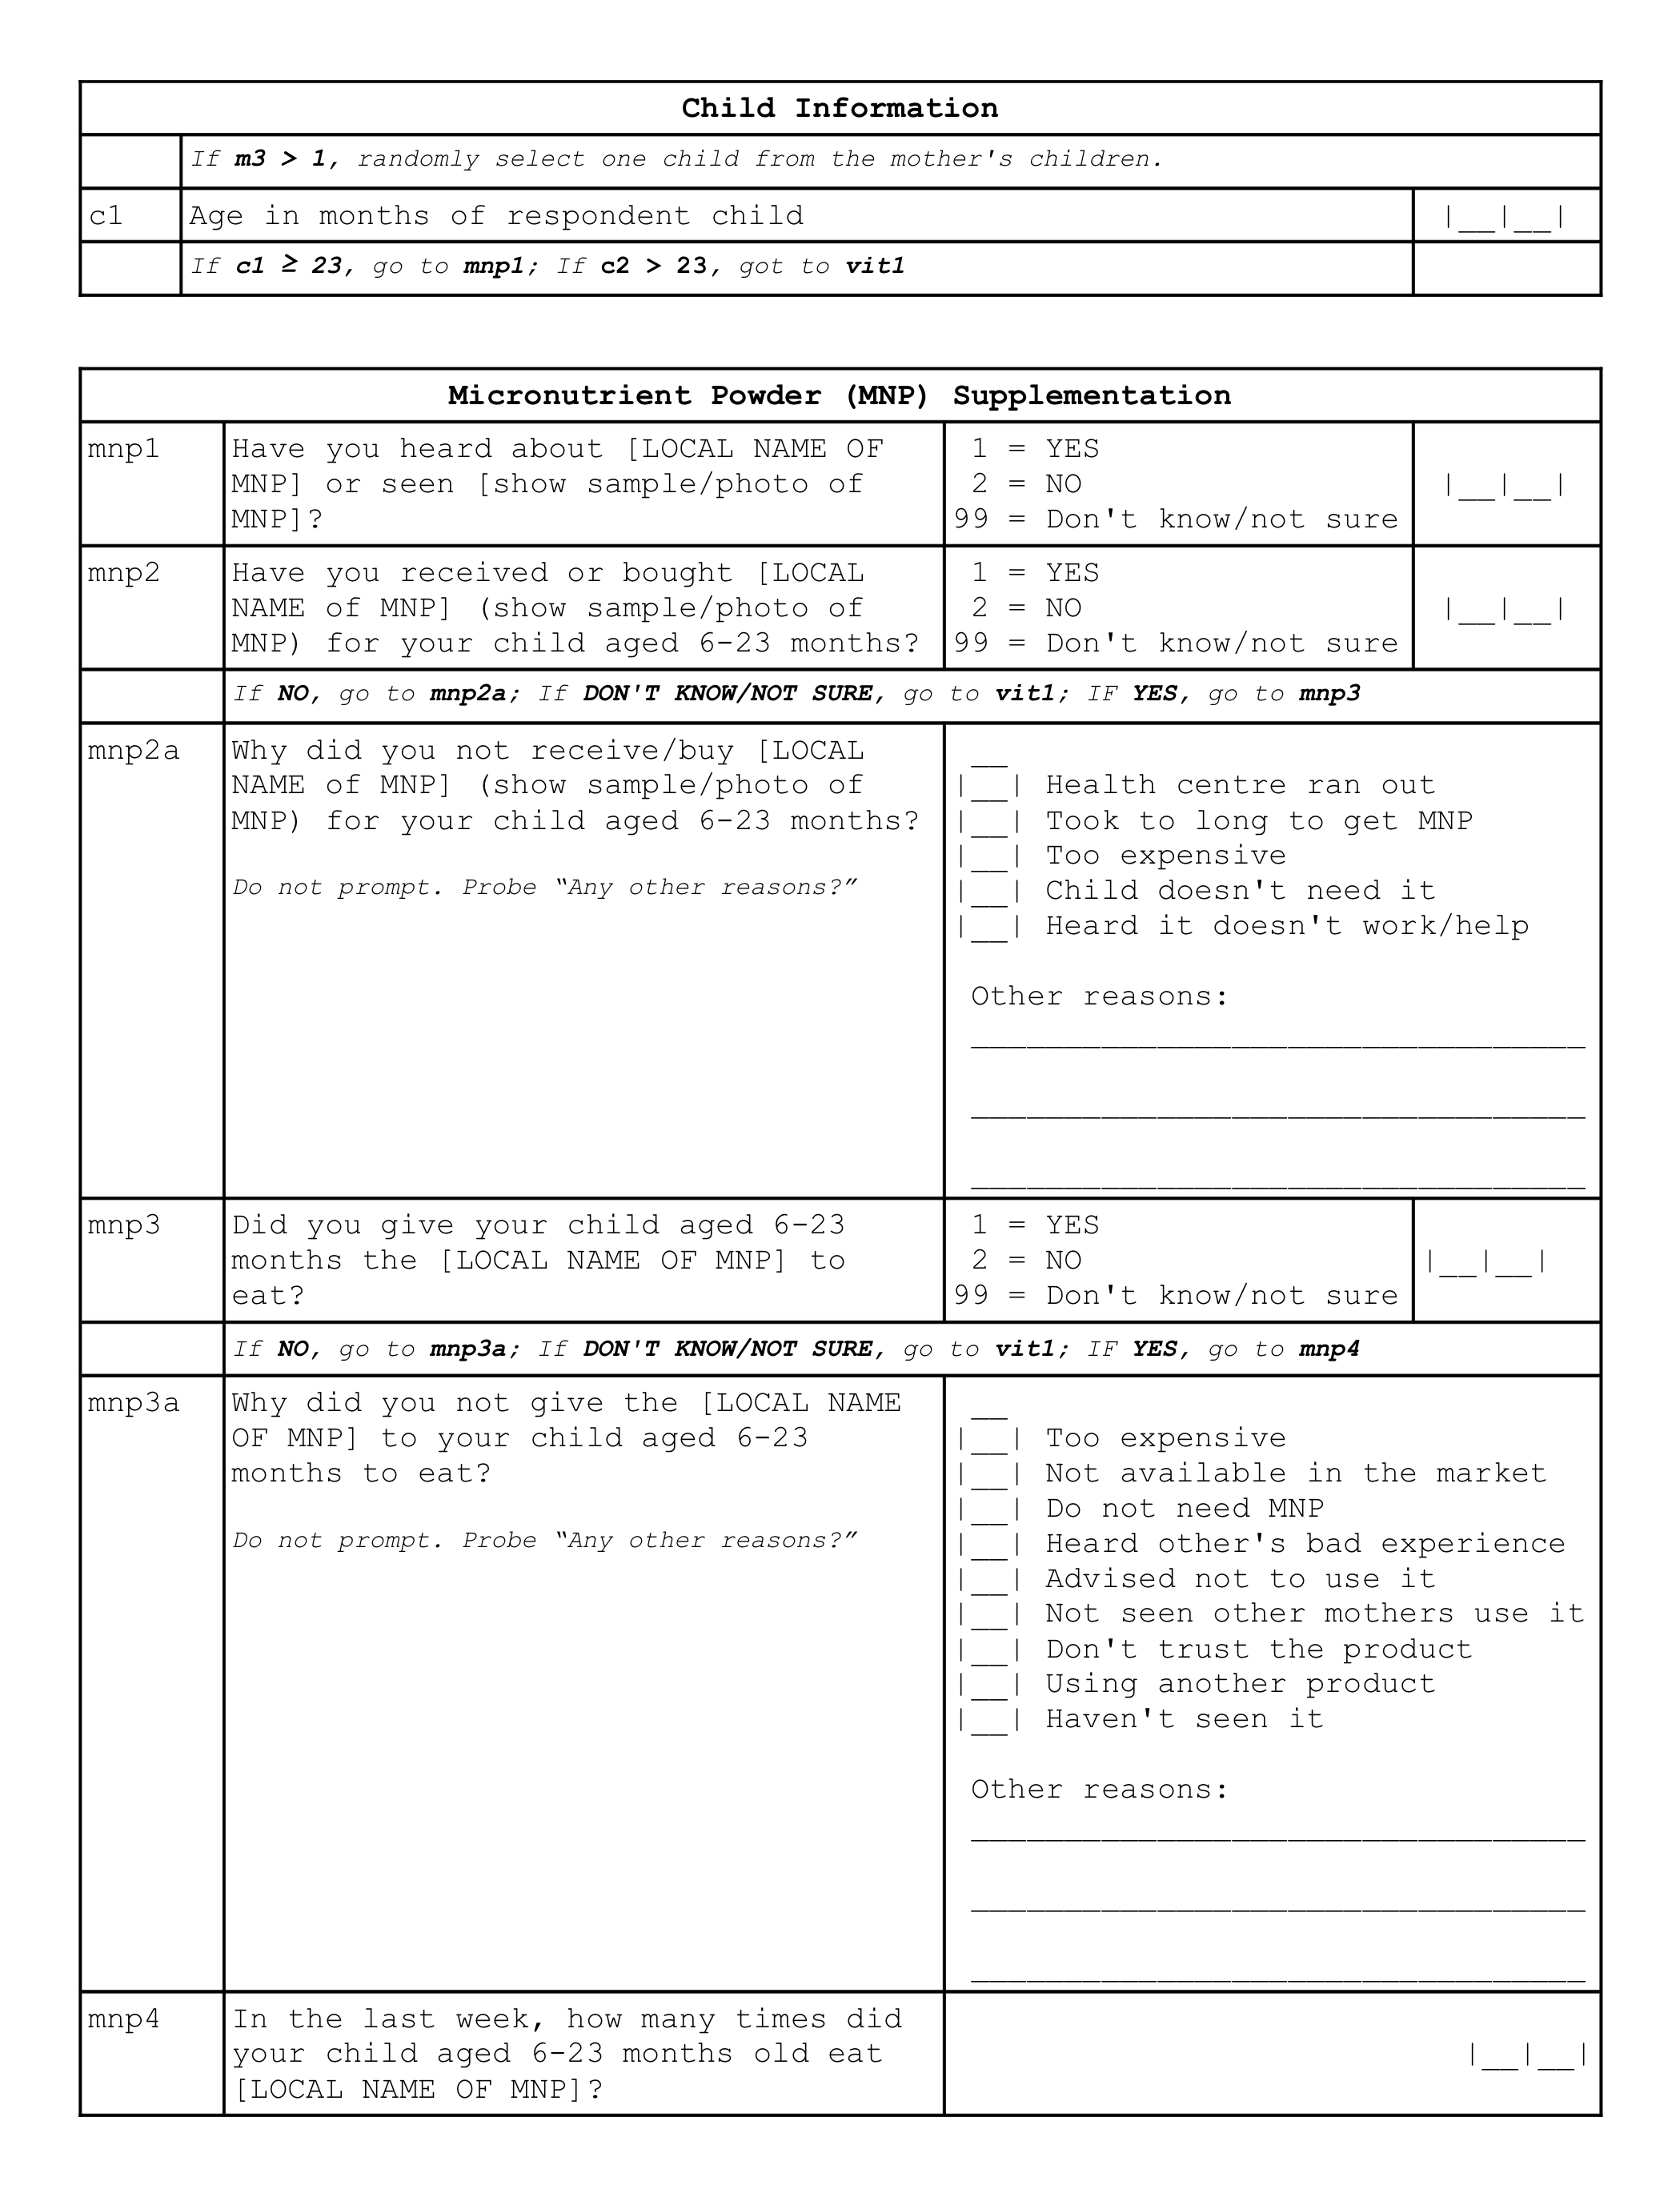
\includegraphics[width=0.9\linewidth]{forms/childForm3} \end{center}

\begin{center}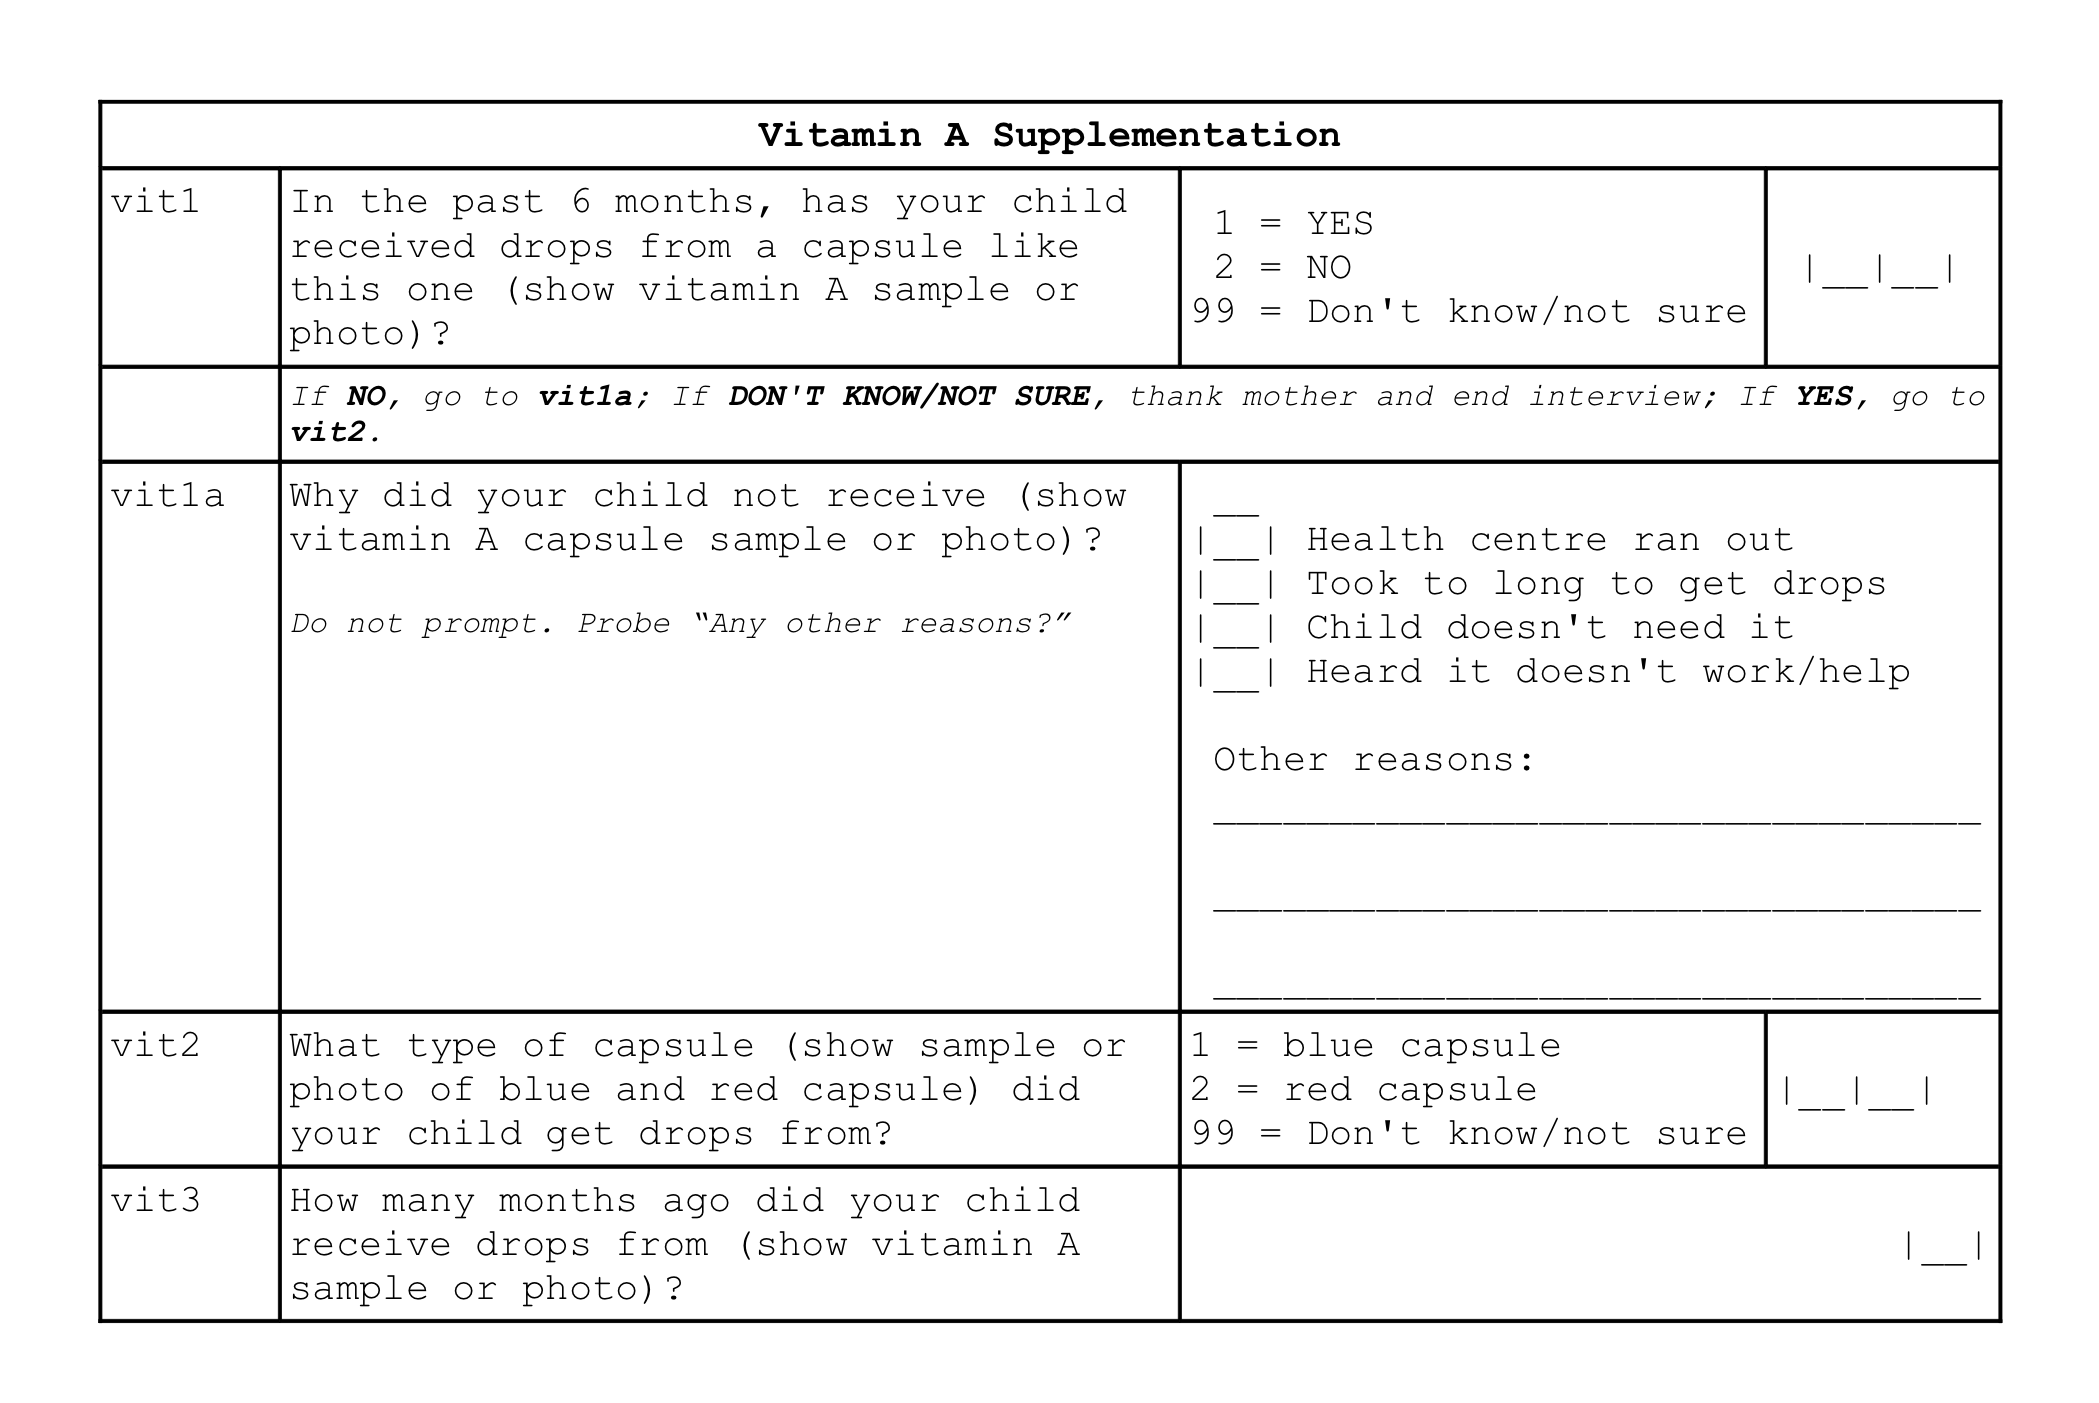
\includegraphics[width=0.9\linewidth]{forms/childForm4} \end{center}

\newpage

\renewcommand\refname{References}
\bibliography{bibliography.bib}


\end{document}
